\documentclass[reqno]{amsart}
%\usepackage{hyperref}
\usepackage{fullpage}
\usepackage{amsrefs}
\usepackage{verbatim}
\usepackage{tikz}
\usepackage{graphicx}

\usetikzlibrary{knots,intersections,decorations.pathreplacing,hobby,arrows}
\tikzset{every path/.style={blue,very thick}, every node/.style={transform shape, knot crossing, inner sep=2.5pt}}

\usepackage[type={CC},modifier={by-nc-sa},version={3.0}]{doclicense}

\newif\ifscreen
\newif\iftwo
\newif\ifshowall
\newif\ifshowkeys
\screenfalse
\twotrue
\showallfalse
\showkeystrue

\input xypic

\ifshowkeys
\newcommand{\lbl}[1]{\label{#1}\textup{[\texttt{#1}]}\ \\}
\else
\newcommand{\lbl}{\label}
\fi

\newcommand{\Braid}     {\operatorname{Braid}}

\newcommand{\N}         {\mathbb{N}}
\newcommand{\Z}         {\mathbb{Z}}
\newcommand{\R}         {\mathbb{R}}
\newcommand{\C}         {\mathbb{C}}

\newcommand{\al}        {\alpha}
\newcommand{\bt}        {\beta}
\newcommand{\ep}        {\epsilon}
\newcommand{\tht}       {\theta}

\newcommand{\Sg}        {\Sigma}

\newcommand{\ab}        {\overline{a}}
\newcommand{\bb}        {\overline{b}}
\newcommand{\cb}        {\overline{c}}
\newcommand{\db}        {\overline{d}}
\newcommand{\eb}        {\overline{e}}
\newcommand{\fb}        {\overline{f}}
\newcommand{\gb}        {\overline{g}}
\newcommand{\pb}        {\overline{p}}
\newcommand{\qb}        {\overline{q}}
\newcommand{\rb}        {\overline{r}}
\newcommand{\ub}        {\overline{u}}
\newcommand{\vb}        {\overline{v}}
\newcommand{\wb}        {\overline{w}}
\newcommand{\xb}        {\overline{x}}
\newcommand{\yb}        {\overline{y}}
\newcommand{\zb}        {\overline{z}}

\newcommand{\tu}        {\widetilde{u}}

\newcommand{\lk}        {\operatorname{lk}}
\newcommand{\ip}[1]     {\langle #1\rangle}
\newcommand{\un}[1]     {\langle\!\langle #1\rangle\!\rangle}
\newcommand{\st}        {\;|\;}
\newcommand{\tm}        {\times}
\newcommand{\ov}        {\overline}
\newcommand{\sse}       {\subseteq}
\newcommand{\sm}        {\setminus}

\renewcommand{\:}       {\colon}


\tikzset{every path/.style={blue,ultra thick}, every node/.style={transform shape, knot crossing, inner sep=2.5pt}}


\newtheorem{theorem}{Theorem}[section]
\newtheorem{conj}[theorem]{Conjecture}
\newtheorem{lemma}[theorem]{Lemma}
\newtheorem{proposition}[theorem]{Proposition}
\newtheorem{corollary}[theorem]{Corollary}
\theoremstyle{definition}
\newtheorem{remark}[theorem]{Remark}
\newtheorem{predefinition}[theorem]{Predefinition}
\newtheorem{definition}[theorem]{Definition}
\newtheorem{example}[theorem]{Example}
\newtheorem{algorithm}[theorem]{Algorithm}
\newtheorem{method}[theorem]{Method}
\newtheorem{fact}[theorem]{Fact}
% Exercises are numbered separately
\newtheorem{exercise}{Exercise}[section]

%\renewenvironment{solution}{\SolutionAtEnd}{\endSolutionAtEnd}
%\renewenvironment{solution}{\SolutionHidden}{\endSolutionHidden}

\newwrite\refs
\openout\refs=\jobname.refs
\makeatletter
\renewcommand\@setref[3]{%
        \ifx#1\relax
                \write\refs{'#3' \thepage\space undefined}%
                \protect \G@refundefinedtrue
                \nfss@text{\reset@font\bfseries ??}%
                \@latex@warning{Reference `#3' on page \thepage\space
                                undefined}%
        \else
                \begingroup
                \count@\expandafter\@secondoftwo#1\relax
                \ifnum\c@page<\count@
                        \write\refs{'#3' \thepage\space
                                    \expandafter\@secondoftwo#1}%
                \fi
                \endgroup
                \expandafter#2#1\null
        \fi
}
\makeatother

\newcommand{\dfn}[1]{\emph{{#1}}\index{#1}}
\newcommand{\idx}[1]{{#1}\index{#1}}

\makeindex

\begin{document}

\title{Knots and Surfaces}
\author{Neil Strickland}

\maketitle

\begin{center}
 This work is licensed under a 
 \href{https://creativecommons.org/licenses/by-nc-sa/3.0/deed.en}{
  Creative Commons Attribution-NonCommercial-ShareAlike license}.
 
 \bigskip

 \doclicenseImage 
\end{center}

%\tableofcontents 

\section{Introduction to knots}
\label{sec-knot-intro}

The first half of this course is about the mathematical theory of
knots, and especially an invariant called the Jones polynomial.

To explain what is meant by a mathematical knot, consider the two
pictures below. \\[2ex]  
\begin{center}
 \begin{tikzpicture}[scale=0.4]
  \node (a) at (-1.00, 0.00) {};
  \node (b) at ( 1.00, 0.00) {};
  \node (c) at ( 0.00, 0.50) {};
  \draw (-4,0) -- (a)
    .. controls (a.2 east) and (c.south west) .. (c.center)
    .. controls (c.4 north east) and (b.4 north) .. (b)
    .. controls (b.8 south) and (a.8 south) .. (a.center)
    .. controls (a.4 north) and (c.4 north west) .. (c)
    .. controls (c.south east) and (b.2 west) .. (b.center)
    -- (4,0);
 \end{tikzpicture}
 \hspace{4em}
 \begin{tikzpicture}[scale=0.4]
  \node (a) at (-1.00, 0.00) {};
  \node (b) at ( 1.00, 0.00) {};
  \node (c) at ( 0.00, 0.50) {};
  \draw (-4,0) -- (a)
    .. controls (a.2 east) and (c.south west) .. (c.center)
    .. controls (c.4 north east) and (b.4 north) .. (b)
    .. controls (b.8 south) and (a.8 south) .. (a.center)
    .. controls (a.4 north) and (c.4 north west) .. (c)
    .. controls (c.south east) and (b.2 west) .. (b.center)
    -- (4,0);
  \draw[rounded corners]
   (4,0) -- (4.2,0) -- (4.2,1.5) -- (-4.2,1.5) -- (-4.2,0) -- (-4,0);
 \end{tikzpicture}
\end{center}
Both pictures show curves embedded in $\R^3$.  The left hand picture
is not considered to be a knot, because it can be untied, but the
right hand picture shows a knot.  

This is one of several closely related concepts, which are illustrated
by the pictures below.
\begin{center}
 \begin{tikzpicture}[scale=0.5]
  \begin{scope}
   \begin{scope}[rotate=  0] \node (a0) at (0,1) {}; \end{scope}
   \begin{scope}[rotate=120] \node (a1) at (0,1) {}; \end{scope}
   \begin{scope}[rotate=240] \node (a2) at (0,1) {}; \end{scope}
   \begin{scope}[rotate= 60] \node (b0) at (0,2) {}; \end{scope}
   \begin{scope}[rotate=180] \node (b1) at (0,2) {}; \end{scope}
   \begin{scope}[rotate=300] \node (b2) at (0,2) {}; \end{scope}
   \draw[blue]
         (b0)        .. controls (b0.4 south west) and (a1.4 north east) ..
         (a1.center) .. controls (a1.4 south west) and (a2.4 south east) ..
         (a2)        .. controls (a2.4 north west) and (b2.4 south east) ..
         (b2.center) .. controls (b2.16 north west) and (b0.16 north east) .. (b0);
   \draw[red]
         (b1)        .. controls (b1.4 south west) and (a2.4 north east) ..
         (a2.center) .. controls (a2.4 south west) and (a0.4 south east) ..
         (a0)        .. controls (a0.4 north west) and (b0.4 south east) ..
         (b0.center) .. controls (b0.16 north west) and (b1.16 north east) .. (b1);
   \draw[green]
         (b2)        .. controls (b2.4 south west) and (a0.4 north east) ..
         (a0.center) .. controls (a0.4 south west) and (a1.4 south east) ..
         (a1)        .. controls (a1.4 north west) and (b1.4 south east) ..
         (b1.center) .. controls (b1.16 north west) and (b2.16 north east) .. (b2);
   \draw[blue ,->] ( 90:2.7) -- +(180:0.1); 
   \draw[red  ,->] (210:2.7) -- +(300:0.1); 
   \draw[green,->] (330:2.7) -- +(420:0.1); 
  \end{scope}
  \begin{scope}[xshift=6cm]
   \node (a) at ( 0.0, 1.5) {};
   \node (b) at ( 0.0, 0.5) {};
   \node (c) at ( 0.0,-0.5) {};
   \node (d) at ( 0.0,-1.5) {};
   \node (e) at ( 4.0, 1.0) {};
   \node (f) at ( 4.0,-1.0) {};
   \node (p) at ( 2.6, 1.0) {};
   \node (q) at ( 2.0, 0.3) {};
   \node (r) at ( 1.4,-0.3) {};
   \node (s) at ( 0.8,-1.0) {};

   \fill[lightgray] (-0.5,-1.8) rectangle ( 0.0, 1.8);
   \fill[lightgray] ( 4.0,-1.8) rectangle ( 4.5, 1.8);
   \draw[blue] 
    (a.center) .. controls (a.4 east) and (p.8 north east) ..
    (p)        .. controls (p.4 south west) and (q.4 north east) ..
    (q.center) .. controls (q.4 south west) and (r.4 north east) ..
    (r)        .. controls (r.4 south west) and (s.4 north east) ..
    (s.center) .. controls (s.4 south west) and (d.4 east) ..
    (d.center);
   \draw[red]
    (b.center) .. controls (b.4 east) and (r.4 north west) ..
    (r.center) .. controls (r.4 south east) and (q.4 south east) .. 
    (q)        .. controls (q.4 north west) and (p.4 north west) ..
    (p.center) .. controls (p.4 south east) and (e.4 west) ..
    (e.center);
   \draw[green]
    (c.center) .. controls (c.4 east) and (s.4 north west) ..
    (s)        .. controls (s.4 south east) and (f.4 west) ..
    (f.center);
  \end{scope}
  \begin{scope}[xshift=14cm]
   \node (a) at (0, 2) {};
   \node (b) at (0, 1) {};
   \node (c) at (0, 0) {};
   \node (d) at (0,-1) {};
   \node (e) at (0,-2) {};
   \node (f) at (9, 2) {};
   \node (g) at (9, 1) {};
   \node (h) at (9, 0) {};
   \node (i) at (9,-1) {};
   \node (j) at (9,-2) {};
   \node (p) at ( 3.5, 1.5) {};
   \node (q) at ( 4.5, 1.5) {};
   \node (r) at ( 2.5, 0.5) {};
   \node (s) at ( 5.5, 0.5) {};
   \node (t) at ( 7.5, 0.5) {};
   \node (u) at ( 1.5,-0.5) {};
   \node (v) at ( 2.5,-1.5) {};
   \node (w) at ( 3.5,-1.5) {};
   \node (x) at ( 4.5,-1.5) {};
   \node (y) at ( 6.5,-0.5) {};

   \fill[lightgray] (-0.5,-2.3) rectangle ( 0.0, 2.3);
   \fill[lightgray] ( 9.0,-2.3) rectangle ( 9.5, 2.3);

   \draw[blue] 
    (a.center) .. controls (a.16 east) and (p.4 north west) ..
    (p.center) .. controls (p.4 south east) and (q.4 south west) ..
    (q)        .. controls (q.4 north east) and (f.16 west) ..
    (f.center);

   \draw[red]
    (b.center) .. controls (b.4 east) and (r.4 north west) ..
    (r.center) .. controls (r.4 south east) and (s.4 south west) ..
    (s)        .. controls (s.4 north east) and (t.4 north west) ..
    (t.center) .. controls (t.4 south east) and (h.4 west) ..
    (h.center);

   \draw[green] 
    (c.center) .. controls (c.4 east) and (u.4 north west) ..
    (u)        .. controls (u.4 south east) and (v.4 north west) ..
    (v.center) .. controls (v.4 south east) and (w.4 south west) ..
    (w)        .. controls (w.4 north east) and (x.4 north west) ..
    (x.center) .. controls (x.4 south east) and (j.16 west) ..
    (j.center);

   \draw[magenta] 
    (d.center) .. controls (d.4 east) and (u.4 south west) ..
    (u.center) .. controls (u.4 north east) and (r.4 south west) ..
    (r)        .. controls (r.4 north east) and (p.4 south west) ..
    (p)        .. controls (p.4 north east) and (q.4 north west) ..
    (q.center) .. controls (q.4 south east) and (s.4 north west) ..
    (s.center) .. controls (s.4 south east) and (y.4 north west) ..
    (y.center) .. controls (y.4 south east) and (i.4 west) ..
    (i.center);

   \draw[cyan] 
    (e.center) .. controls (e.8 east) and (v.4 south west) ..
    (v)        .. controls (v.4 north east) and (w.4 north west) ..
    (w.center) .. controls (w.4 south east) and (x.4 south west) ..
    (x)        .. controls (x.4 north east) and (y.4 south west) ..
    (y)        .. controls (y.4 north east) and (t.4 south west) ..
    (t)        .. controls (t.4 north east) and (g.4 west) ..
    (g.center);
  \end{scope}
  \begin{scope}[scale=2,yshift=-1.8cm,draw=black]
   \draw[black] (-0.3,0) node {a link};
   \draw[black] ( 4.0,0) node {a tangle};
   \draw[black] ( 9.0,0) node {a braid};
  \end{scope}
 \end{tikzpicture}
\end{center}
\medskip
The first hand picture shows a \emph{link}, which is like a knot but
which may have more than one strand.  (Knots are considered to be a
special case of links.)  The second picture shows a \emph{tangle},
which is like a link, but the strands have ends, which are fixed to
walls on the left or the right.  The third picture shows a
\emph{braid}, which is a special kind of tangle in which all run from
left to right without ever curling backwards.  Braids are nice because
if we have two braids with $n$ strands then we can join them together
to make a new braid with $n$ strands, and this operation makes the set
of $n$-stranded braids into a group.  We can convert braids into links
by joining the left ends to the right ends in an obvious pattern, as
illustrated below:\\[2ex]
\begin{center}
 \begin{tikzpicture}[scale=0.5]
  \node (a) at (0, 2) {};
  \node (b) at (0, 1) {};
  \node (c) at (0, 0) {};
  \node (d) at (0,-1) {};
  \node (e) at (0,-2) {};
  \node (f) at (9, 2) {};
  \node (g) at (9, 1) {};
  \node (h) at (9, 0) {};
  \node (i) at (9,-1) {};
  \node (j) at (9,-2) {};
  \node (p) at ( 3.5, 1.5) {};
  \node (q) at ( 4.5, 1.5) {};
  \node (r) at ( 2.5, 0.5) {};
  \node (s) at ( 5.5, 0.5) {};
  \node (t) at ( 7.5, 0.5) {};
  \node (u) at ( 1.5,-0.5) {};
  \node (v) at ( 2.5,-1.5) {};
  \node (w) at ( 3.5,-1.5) {};
  \node (x) at ( 4.5,-1.5) {};
  \node (y) at ( 6.5,-0.5) {};

  \draw
   (a.center) .. controls (a.16 east) and (p.4 north west) ..
   (p.center) .. controls (p.4 south east) and (q.4 south west) ..
   (q)        .. controls (q.4 north east) and (f.16 west) ..
   (f.center);

  \draw[red]
   (b.center) .. controls (b.4 east) and (r.4 north west) ..
   (r.center) .. controls (r.4 south east) and (s.4 south west) ..
   (s)        .. controls (s.4 north east) and (t.4 north west) ..
   (t.center) .. controls (t.4 south east) and (h.4 west) ..
   (h.center);

  \draw[red]
   (c.center) .. controls (c.4 east) and (u.4 north west) ..
   (u)        .. controls (u.4 south east) and (v.4 north west) ..
   (v.center) .. controls (v.4 south east) and (w.4 south west) ..
   (w)        .. controls (w.4 north east) and (x.4 north west) ..
   (x.center) .. controls (x.4 south east) and (j.16 west) ..
   (j.center);

  \draw[red]
   (d.center) .. controls (d.4 east) and (u.4 south west) ..
   (u.center) .. controls (u.4 north east) and (r.4 south west) ..
   (r)        .. controls (r.4 north east) and (p.4 south west) ..
   (p)        .. controls (p.4 north east) and (q.4 north west) ..
   (q.center) .. controls (q.4 south east) and (s.4 north west) ..
   (s.center) .. controls (s.4 south east) and (y.4 north west) ..
   (y.center) .. controls (y.4 south east) and (i.4 west) ..
   (i.center);

  \draw[red]
   (e.center) .. controls (e.8 east) and (v.4 south west) ..
   (v)        .. controls (v.4 north east) and (w.4 north west) ..
   (w.center) .. controls (w.4 south east) and (x.4 south west) ..
   (x)        .. controls (x.4 north east) and (y.4 south west) ..
   (y)        .. controls (y.4 north east) and (t.4 south west) ..
   (t)        .. controls (t.4 north east) and (g.4 west) ..
   (g.center);

  \draw[rounded corners] (0, 2) -- (-1.8, 2) -- (-1.8,-3.8) -- (10.8,-3.8) -- (10.8, 2) -- (9, 2);
  \draw[red,rounded corners] (0, 1) -- (-1.6, 1) -- (-1.6,-3.6) -- (10.6,-3.6) -- (10.6, 1) -- (9, 1);
  \draw[red,rounded corners] (0, 0) -- (-1.4, 0) -- (-1.4,-3.4) -- (10.4,-3.4) -- (10.4, 0) -- (9, 0);
  \draw[red,rounded corners] (0,-1) -- (-1.2,-1) -- (-1.2,-3.2) -- (10.2,-3.2) -- (10.2,-1) -- (9,-1);
  \draw[red,rounded corners] (0,-2) -- (-1,-2) -- (-1,-3) -- (10,-3) -- (10,-2) -- (9,-2);
 \end{tikzpicture}
\end{center}

This course will focus on knots and links, with occasional comments on
tangles and braids.

We will consider two links to be equivalent if one can be deformed
into the other.  For example, the knot shown on the left below can
easily be deformed into an unknotted circle as shown on the right, so
we will not distinguish between them.
\begin{center}
 \begin{tikzpicture}[scale=0.7]
  \begin{scope}
   \node (a) at (-1.00, 1.00) {};
   \node (b) at ( 1.00, 1.00) {};
   \node (c) at ( 0.00, 0.00) {};
   \node (d) at (-1.00,-1.00) {};
   \node (e) at ( 1.00,-1.00) {};
   \node (f) at ( 0.00,-2.00) {};
   \draw (a) -- (c.center) -- (e)
    .. controls (e.4 south east) and (f.4 south east) .. (f) -- (d.center)
    .. controls (d.4 north west) and (a.4 south west) .. (a.center) 
    .. controls (a.4 north east) and (b.4 north west) .. (b.center) 
    .. controls (b.4 south east) and (e.4 north east) .. (e.center) -- (f.center)
    .. controls (f.4 south west) and (d.4 south west) .. (d) 
    -- (c) -- (b) 
    .. controls (b.8 north east) and (a.8 north west) .. (a);
  \end{scope}
  \begin{scope}[xshift=5cm]
   \draw (0,0) circle(1);
  \end{scope}
 \end{tikzpicture}
\end{center}

We next discuss how to make our definitions more formal.  There are
two problems that we need to work around.  The first issue is that
there are things that are similar to knots but have infinite
complexity, like this:
\begin{center}
 \begin{tikzpicture}[scale=0.7]
  \begin{scope}
   \node (a) at (-1.00, 0.00) {};
   \node (b) at ( 1.00, 0.00) {};
   \node (c) at ( 0.00, 0.50) {};
   \draw (-2,0) -- (a)
     .. controls (a.2 east) and (c.south west) .. (c.center)
     .. controls (c.4 north east) and (b.4 north) .. (b)
     .. controls (b.8 south) and (a.8 south) .. (a.center)
     .. controls (a.4 north) and (c.4 north west) .. (c)
     .. controls (c.south east) and (b.2 west) .. (b.center)
     -- (2,0);
  \end{scope}
  \begin{scope}[scale=0.5,xshift=5cm]
   \node (a) at (-1.00, 0.00) {};
   \node (b) at ( 1.00, 0.00) {};
   \node (c) at ( 0.00, 0.50) {};
   \draw (-2,0) -- (a)
     .. controls (a.2 east) and (c.south west) .. (c.center)
     .. controls (c.4 north east) and (b.4 north) .. (b)
     .. controls (b.8 south) and (a.8 south) .. (a.center)
     .. controls (a.4 north) and (c.4 north west) .. (c)
     .. controls (c.south east) and (b.2 west) .. (b.center)
     -- (2,0);
  \end{scope}
  \begin{scope}[scale=0.25,xshift=15cm]
   \node (a) at (-1.00, 0.00) {};
   \node (b) at ( 1.00, 0.00) {};
   \node (c) at ( 0.00, 0.50) {};
   \draw (-2,0) -- (a)
     .. controls (a.2 east) and (c.south west) .. (c.center)
     .. controls (c.4 north east) and (b.4 north) .. (b)
     .. controls (b.8 south) and (a.8 south) .. (a.center)
     .. controls (a.4 north) and (c.4 north west) .. (c)
     .. controls (c.south east) and (b.2 west) .. (b.center)
     -- (2,0);
  \end{scope}
  \begin{scope}[scale=0.125,xshift=36cm]
   \node (a) at (-1.00, 0.00) {};
   \node (b) at ( 1.00, 0.00) {};
   \node (c) at ( 0.00, 0.50) {};
   \draw (-2,0) -- (a)
     .. controls (a.2 east) and (c.south west) .. (c.center)
     .. controls (c.4 north east) and (b.4 north) .. (b)
     .. controls (b.8 south) and (a.8 south) .. (a.center)
     .. controls (a.4 north) and (c.4 north west) .. (c)
     .. controls (c.south east) and (b.2 west) .. (b.center)
     -- (2,0);
  \end{scope}
  \draw[dotted] (4.8,0) -- (5.5,0);
  \draw[rounded corners] (5.5,0) -- (6,0) -- (6,2) -- (-2,2) -- (-2,0) -- (-1,0);
 \end{tikzpicture}
\end{center}

(This is supposed to show an infinite sequence of knotted loops, where
the $n$'th loop has size $2^{-n}$.)  We only want to study knots of
finite complexity, so we should arrange our definitions so that the
above picture does not count as a knot.  

The second issue is closely related.  Suppose we have a knot in a thin
piece of cotton thread.  If we pull it tight, the knot will disappear,
becoming a small bump on the thread.  Mathematical knots are
considered to be made from infinitely thin thread, so if we pull them
tight, there will not even be a bump.  We should arrange our
definitions so that knots cannot just disappear like this.

Unfortunately, a really complete and rigorous account of the
definitions would take a long time, and would not shed that much light
on the main questions of interest in this course.  We will therefore
just just give an indication of the main points.  

\begin{definition}
 If $a$ and $b$ are points in $\R^3$ with $a\neq b$, we put 
 \[ [a,b] = \text{ the line segment between $a$ and $b$ } 
     = \{(1-t)a+tb\st 0\leq t\leq 1\} \subset\R^3.
 \]
 Now consider a subset $L\subset\R^3$.  We say that $L$ is a
 \emph{piecewise linear link} if it can be written as a finite union
 of line segments as above, say $L=S_1\cup\dotsb\cup S_n$, in such a
 way that
 \begin{itemize}
  \item[(a)] If $i\neq j$ then either $S_i\cap S_j=\emptyset$, or
   there is a point $x$ which is an endpoint of $S_i$ and also an
   endpoint of $S_j$, such that $S_i\cap S_j=\{x\}$.
  \item[(b)] For each $i$, and for each endpoint $x$ of $S_i$, there
   is precisely one other index $j$ such that $x$ is also an endpoint
   of $S_j$.
 \end{itemize}
\end{definition}

In other words, a piecewise linear link is a link of the type that we
have illustrated previously, except that the strands can be divided
into a finite number of straight sections.  We would like to say that
any link (of finite complexity) can be be deformed into a piecewise
linear one.  For this, we need a formal definition of the kind of
deformation that we want to consider.

\begin{definition}
 \begin{itemize}
  \item[(a)] A \emph{homeomorphism} of $\R^n$ is a bijective map
   $f\:\R^n\to\R^n$ such that both $f$ and $f^{-1}$ are continuous.
  \item[(b)] Suppose we have a family of homeomorphisms
   $f_t\:\R^n\to\R^n$ for $0\leq t\leq 1$, and we define maps
   $h,h^*\:[0,1]\tm\R^n\to\R^n$ by $h(t,x)=f_t(x)$ and
   $h^*(t,x)=f_t^{-1}(x)$.  We say that the maps $f_t$ form an
   \emph{isotopy} of $\R^n$ if $h$ and $h^*$ are continuous, and
   $f_0(x)=x$ for all $x$.
  \item[(c)] Let $X$ and $Y$ be two subsets of $\R^n$.  We say that
   they are \emph{ambiently isotopic} if there is an isotopy as in~(b)
   with $f_1(X)=Y$.  (It is not hard to check that this is an
   equivalence relation.)
  \item[(d)] A \emph{link} is a subset of $\R^3$ that is ambiently
   isotopic to a piecewise linear link.  We say that two links are
   \emph{equivalent} if they are ambiently isotopic.
 \end{itemize}
\end{definition}

\section{Why study knots?}
\label{sec-why-knots}

Firstly, knots are a good introductory example of topological
phenomena.  There are many examples in mathematics where objects can
be deformed continuously in infinitely many different ways, but there
are some discrete properties that always remain the same, such as the
number of strands, and certain aspects of the way they twist around
each other.  The theories of algebraic topology, differential topology
and homotopy theory have a huge literature devoted to this kind of
phenomenon.  Knot theory is in some respects the simplest example that
one can study.  Moreover, knot theory can also be used indirectly to
shed light on other kinds of topological questions.  For example,
there is a construction called \emph{Dehn surgery} which allows one to
create new kinds of three-dimensional spaces by taking $\R^3$ and
``twisting it around a knot''.  

Next, there are some unexpected connections with other areas of pure
mathematics.  As we mentioned previously, braids with $n$ strands form
a group, called $\Braid_n$.  For various reasons it is interesting to
consider homomorphisms $\rho\:\Braid_n\to GL_d(\C)$ (where $d$ is a
natural number, and $GL_d(\C)$ is the group of invertible $d\tm d$
matrices over the complex numbers); these are called \emph{linear
 representations} of the braid group.  It turns out that the
representation theory of the braid group is closely related to knot
theory, and also to some questions in statistical physics and
functional analysis.  A significant part of this course will be
devoted to studying the Jones polynomial of a knot.  Historically,
this was first invented by Vaughan Jones as a byproduct of his work in
these areas; he was not originally studying knots at all.

Finally, there are a number of places where knotting occurs in
nature.  Strands of DNA sometimes become knotted, and biologists have
investigated what this tells us about the means by which DNA is
manipulated in cells.  Magnetic field lines can be knotted,
particularly in the extreme magnetic conditions that can arise in
astrophysics.

In the late nineteenth century there was actually a popular theory,
proposed by the physicist Kelvin, that atoms were actually knotted
structures in a hypothetical substance called aether that was thought
to carry light waves.  This is an attractive theory, because it would
explain the discrete series of different elements in terms of a
discrete series of different knot types.  Although it did not turn out
to be correct, it did inspire some foundational work in knot theory.
Moreover, there are echoes of Kelvin's idea in the much newer physical
theory of ``strings''.  This theory (which may or may not be on the
right track) aims to unify all the fundamental forces of nature, and
has been the focus of an enormous body of work by physicists over
several decades.  It also rests heavily on topological ideas, starting
with the theory of surfaces which forms the second half of this course
(but continuing well beyond that).

\section{Invariants}
\label{sec-invariants}

Consider the following knots:
\begin{center}
 \begin{tikzpicture}[scale=0.7]
  \begin{scope}[scale=0.6]
   \draw (0,0) circle(2.6);
   \begin{scope}[rotate=  0] \node (a) at (0,-1) {}; \end{scope}
   \begin{scope}[rotate=120] \node (b) at (0,-1) {}; \end{scope}
   \begin{scope}[rotate=240] \node (c) at (0,-1) {}; \end{scope}
   \draw (a) .. controls (a.4 north west) and (c.4 north east) .. (c.center);
   \draw (b) .. controls (b.4 north west) and (a.4 north east) .. (a.center);
   \draw (c) .. controls (c.4 north west) and (b.4 north east) .. (b.center);
   \draw (a.center) .. controls (a.16 south west) and (c.16 south east) .. (c);
   \draw (b.center) .. controls (b.16 south west) and (a.16 south east) .. (a);
   \draw (c.center) .. controls (c.16 south west) and (b.16 south east) .. (b);
   \fill[white] (-0.3,1.2) rectangle (0.3,2.7);
   \draw (-0.3,2.60) -- (0.3,2.17);
   \draw (-0.3,2.17) -- (-0.1,2.33);
   \draw ( 0.3,2.60) -- ( 0.1,2.48);
  \end{scope}
  \begin{scope}[xshift=5cm,scale=1.4]
   \node (a) at ( 0.00, 1.00) {};
   \node (b) at ( 0.00, 0.00) {};
   \node (c) at ( 0.00,-1.00) {};
   \draw (a.center) 
    .. controls (a.4 south east) and (b.4 north east) .. (b) 
    .. controls (b.4 south west) and (c.4 north west) .. (c.center) 
    .. controls (c.8 south east) and (a.8 north east) .. (a)
    .. controls (a.4 south west) and (b.4 north west) .. (b.center)
    .. controls (b.4 south east) and (c.4 north east) .. (c)
    .. controls (c.8 south west) and (a.8 north west) .. (a.center);
  \end{scope}
  \begin{scope}[xshift=10cm,scale=0.5]
   \begin{scope}[rotate=  0] \node (a) at (0,-1.5) {}; \end{scope}
   \begin{scope}[rotate= 72] \node (b) at (0,-1.5) {}; \end{scope}
   \begin{scope}[rotate=144] \node (c) at (0,-1.5) {}; \end{scope}
   \begin{scope}[rotate=216] \node (d) at (0,-1.5) {}; \end{scope}
   \begin{scope}[rotate=288] \node (e) at (0,-1.5) {}; \end{scope}

   \draw (0,0) 
    (a) .. controls (a.16 south east) and (b.16 south west) .. (b.center) .. controls (b.4 north east) and (c.4 north west) ..
    (c) .. controls (c.16 south east) and (d.16 south west) .. (d.center) .. controls (d.4 north east) and (e.4 north west) ..
    (e) .. controls (e.16 south east) and (a.16 south west) .. (a.center) .. controls (a.4 north east) and (b.4 north west) ..
    (b) .. controls (b.16 south east) and (c.16 south west) .. (c.center) .. controls (c.4 north east) and (d.4 north west) ..
    (d) .. controls (d.16 south east) and (e.16 south west) .. (e.center) .. controls (e.4 north east) and (a.4 north west) ..
    (a); 
  \end{scope}
 \end{tikzpicture}
\end{center}
You can probably convince yourself (with the aid of string if
necessary) that the first two are equivalent to each other, but not to
the third one.  But what about these three?
\begin{center}
 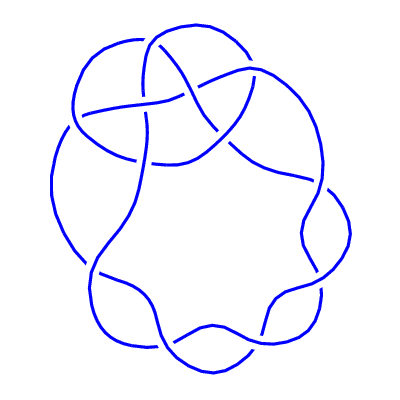
\includegraphics[scale=0.2]{../images/12n_0666.png}\hspace{3em}
 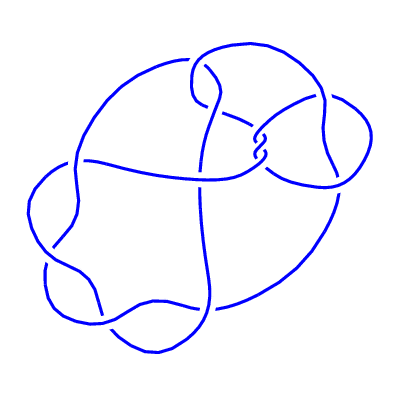
\includegraphics[scale=0.2]{../images/12n_0673.png}\hspace{3em}
 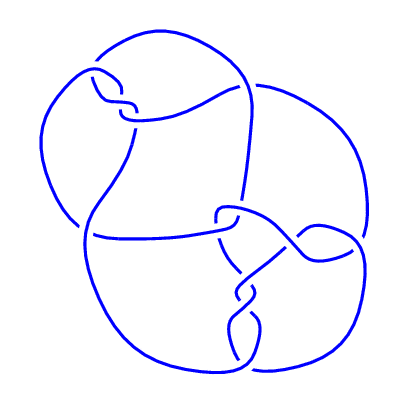
\includegraphics[scale=0.2]{../images/12n_0680.png}
\end{center}
There is no obvious way to deform any of them into any of the others,
but how can we tell if there might be a non-obvious way?  For this, we
need numerical invariants which we can calculate.

For the simplest example, note that any link can be divided into
separate strands, each of which is essentially a circle.  These
strands are called the \emph{components} of the link, and we write
$c(L)$ for the number of components.  The following pictures show a
link with one component, a link with two components and a link with
three components.

\begin{center}
 \begin{tikzpicture}[scale=0.7]
  \begin{scope}
   \node (a) at ( 1,0) {};
   \node (b) at (-1,0) {};
   \draw (a.center) .. controls (a.8 north east) and (b.8 north) ..
         (b.center) .. controls (b.8 south) and (a.8 south east) .. 
         (a) .. controls (a.8 north west) and (a.8 south west) .. (a.center);
  \end{scope}
  \begin{scope}[xshift=5cm]
   \node (a) at ( 0.00, 1.00) {};
   \node (b) at ( 0.00,-1.00) {};
   \draw[blue] (a.center) .. controls (a.4 south east) and (b.4 north east) ..
               (b) .. controls (b.16 south west) and (a.16 north west) .. (a.center);
   \draw[red]  (a) .. controls (a.4 south west) and (b.4 north west) ..
               (b.center) .. controls (b.16 south east) and (a.16 north east) .. (a);
  \end{scope}
  \begin{scope}[xshift=10cm]
   \begin{scope}[rotate=0]
    \draw[blue] (0,0) ( 10:1.3) arc( 10:110:1.3);
    \draw[blue] (0,0) ( 10:0.7) arc( 10:110:0.7);
    \draw[green] (350:1) +( 80:0.3) arc( 80:170:0.3);
    \draw[blue] ( 10:1) +(280:0.3) arc(280:370:0.3);
    \draw[draw=white,double=green,double distance=1.2pt] (350:1) +(350:0.3) arc(-10: 80:0.3);
    \draw[draw=white,double=blue,double distance=1.2pt] ( 10:1) +(190:0.3) arc(190:280:0.3);
   \end{scope}
   \begin{scope}[rotate=120]
    \draw[red] (0,0) ( 10:1.3) arc( 10:110:1.3);
    \draw[red] (0,0) ( 10:0.7) arc( 10:110:0.7);
    \draw[blue] (350:1) +( 80:0.3) arc( 80:170:0.3);
    \draw[red] ( 10:1) +(280:0.3) arc(280:370:0.3);
    \draw[draw=white,double=blue,double distance=1.2pt] (350:1) +(350:0.3) arc(-10: 80:0.3);
    \draw[draw=white,double=red,double distance=1.2pt] ( 10:1) +(190:0.3) arc(190:280:0.3);
   \end{scope}
   \begin{scope}[rotate=240]
    \draw[green] (0,0) ( 10:1.3) arc( 10:110:1.3);
    \draw[green] (0,0) ( 10:0.7) arc( 10:110:0.7);
    \draw[red] (350:1) +( 80:0.3) arc( 80:170:0.3);
    \draw[green] ( 10:1) +(280:0.3) arc(280:370:0.3);
    \draw[draw=white,double=red,double distance=1.2pt] (350:1) +(350:0.3) arc(-10: 80:0.3);
    \draw[draw=white,double=green,double distance=1.2pt] ( 10:1) +(190:0.3) arc(190:280:0.3);
   \end{scope}
  \end{scope}
 \end{tikzpicture}
\end{center}

Suppose we have two links $L$ and $L'$, and we want to decide whether
they are equivalent.  We can start by finding $c(L)$ and $c(L')$
(which is quite easy to do, using any planar picture).  If 
$c(L)\neq c(L')$ then $L$ and $L'$ are definitely not equivalent.
However, if $c(L)=c(L')$ then we have not learned very much; $L$ and
$L'$ might or might not be equivalent.  We therefore need to look for
better invariants.  

As an example of something that does \textbf{not} work, consider the
crossing number.  Given a planar picture $D$ of a knot, we let $n(D)$
denote the number of crossings.  To see what is wrong with this,
consider the following pictures:
\begin{center}
 \begin{tikzpicture}[scale=0.7]
  \begin{scope}[scale=0.8]
   \node (a) at (-1.00, 1.00) {};
   \node (b) at ( 1.00, 1.00) {};
   \node (c) at ( 0.00, 0.00) {};
   \node (d) at (-1.00,-1.00) {};
   \node (e) at ( 1.00,-1.00) {};
   \node (f) at ( 0.00,-2.00) {};
   \draw (a) -- (c.center) -- (e)
    .. controls (e.4 south east) and (f.4 south east) .. (f) -- (d.center)
    .. controls (d.4 north west) and (a.4 south west) .. (a.center) 
    .. controls (a.4 north east) and (b.4 north west) .. (b.center) 
    .. controls (b.4 south east) and (e.4 north east) .. (e.center) -- (f.center)
    .. controls (f.4 south west) and (d.4 south west) .. (d) 
    -- (c) -- (b) 
    .. controls (b.8 north east) and (a.8 north west) .. (a);
  \end{scope}
  \begin{scope}[xshift=5cm]
   \draw (0,0) circle(1);
  \end{scope}
  \begin{scope}[xshift=10cm,scale=0.7]
   \draw (0,0) circle(2.6);
   \begin{scope}[rotate=  0] \node (a) at (0,-1) {}; \end{scope}
   \begin{scope}[rotate=120] \node (b) at (0,-1) {}; \end{scope}
   \begin{scope}[rotate=240] \node (c) at (0,-1) {}; \end{scope}
   \draw (a) .. controls (a.4 north west) and (c.4 north east) .. (c.center);
   \draw (b) .. controls (b.4 north west) and (a.4 north east) .. (a.center);
   \draw (c) .. controls (c.4 north west) and (b.4 north east) .. (b.center);
   \draw (a.center) .. controls (a.16 south west) and (c.16 south east) .. (c);
   \draw (b.center) .. controls (b.16 south west) and (a.16 south east) .. (a);
   \draw (c.center) .. controls (c.16 south west) and (b.16 south east) .. (b);
   \fill[white] (-0.3,1.2) rectangle (0.3,2.7);
   \draw (-0.3,2.60) -- (0.3,2.17);
   \draw (-0.3,2.17) -- (-0.1,2.33);
   \draw ( 0.3,2.60) -- ( 0.1,2.48);
  \end{scope}
  \begin{scope}[xshift=15cm,scale=1.4]
   \node (a) at ( 0.00, 1.00) {};
   \node (b) at ( 0.00, 0.00) {};
   \node (c) at ( 0.00,-1.00) {};
   \draw (a.center) 
    .. controls (a.4 south east) and (b.4 north east) .. (b) 
    .. controls (b.4 south west) and (c.4 north west) .. (c.center) 
    .. controls (c.8 south east) and (a.8 north east) .. (a)
    .. controls (a.4 south west) and (b.4 north west) .. (b.center)
    .. controls (b.4 south east) and (c.4 north east) .. (c)
    .. controls (c.8 south west) and (a.8 north west) .. (a.center);
  \end{scope}
 \end{tikzpicture}
\end{center}
Pictures 1 and 2 show equivalent knots, but picture 1 has 6 crossings
and picture 2 has no crossings.  Similarly, pictures 3 and 4 show
equivalent knots, but picture 3 has 4 crossings and picture 3 has 3
crossings.  Thus, the crossing number is not a well-defined invariant.

We could instead define $n^*(L)$ to be the \emph{minimal crossing
 number} of $L$, or in other words the minimum possible number of
crossings in any planar picture of $L$.  This is an invariant, but it
is very hard to calculate.  If someone gives us a link $L$, there is
no obvious way to list all the possible ways to draw $L$ in the plane,
so we cannot tell how many crossings are needed.

Our aim will be to define an invariant which is quite powerful, and
also quite easy to compute.  

\section{Reidemeister moves}
\label{sec-reidemeister}

We have already drawn many planar pictures of knots and links.  Before
going further, we need to discuss in more detail how such pictures
work.  Our pictures have always had little gaps next to each crossing,
to indicate which strand lies on top.  However, we sometimes need to
consider pictures without this extra information.  These are covered
by the definition below.

\begin{definition}
 A \emph{link universe} is a planar picture, consisting of 
 \begin{itemize}
  \item[(a)] A finite set of points in the plane, called
   \emph{crossings}
  \item[(b)] A set of curves in the plane, called \emph{arcs}.
 \end{itemize}
 These must satisfy the following axioms:
 \begin{itemize}
  \item[(c)] Each arc starts at a crossing, and ends at a crossing
   (possibly the same one).
  \item[(d)] The arcs are disjoint, except that they may intersect at
   the endpoints.
  \item[(e)] For each crossing, there are precisely four half-arcs with
   that crossing as an endpoint.
  \item[(f)] The whole picture is ambient isotopic to a piecewise
   linear one.
 \end{itemize}
\end{definition}

%%% TODO: add extra pictures 

\begin{definition}
 A \emph{link diagram} is a link universe with a choice, for each
 crossing, of which opposite pair of strands lies on top.
\end{definition}

\begin{example}
 The left hand picture below is a link universe.  It has three
 crossings, and at each crossing there are two ways to choose what
 goes on top, so there are $2\tm 2\tm 2=8$ possible link diagrams for
 this universe.  Two of them are shown.  The middle picture is a
 diagram for the trefoil knot.  The right hand picture is the same as
 the middle picture, except that the bottom crossing has been switched
 over.  This allows us to deform the corresponding link into an
 unknotted circle.
 \begin{center}
  \begin{tikzpicture}
   \begin{scope}[scale=0.66]
    \begin{scope}[rotate=  0] \node (a) at (0,-1) {}; \end{scope}
    \begin{scope}[rotate=120] \node (b) at (0,-1) {}; \end{scope}
    \begin{scope}[rotate=240] \node (c) at (0,-1) {}; \end{scope}
    \draw (a.center) .. controls (a.4 north west) and (c.4 north east) .. (c.center);
    \draw (b.center) .. controls (b.4 north west) and (a.4 north east) .. (a.center);
    \draw (c.center) .. controls (c.4 north west) and (b.4 north east) .. (b.center);
    \draw (a.center) .. controls (a.16 south west) and (c.16 south east) .. (c.center);
    \draw (b.center) .. controls (b.16 south west) and (a.16 south east) .. (a.center);
    \draw (c.center) .. controls (c.16 south west) and (b.16 south east) .. (b.center);
   \end{scope}
   \begin{scope}[xshift=4.5cm,scale=0.66]
    \begin{scope}[rotate=  0] \node (a) at (0,-1) {}; \end{scope}
    \begin{scope}[rotate=120] \node (b) at (0,-1) {}; \end{scope}
    \begin{scope}[rotate=240] \node (c) at (0,-1) {}; \end{scope}
    \draw (a) .. controls (a.4 north west) and (c.4 north east) .. (c.center);
    \draw (b) .. controls (b.4 north west) and (a.4 north east) .. (a.center);
    \draw (c) .. controls (c.4 north west) and (b.4 north east) .. (b.center);
    \draw (a.center) .. controls (a.16 south west) and (c.16 south east) .. (c);
    \draw (b.center) .. controls (b.16 south west) and (a.16 south east) .. (a);
    \draw (c.center) .. controls (c.16 south west) and (b.16 south east) .. (b);
   \end{scope}
   \begin{scope}[xshift=9.0cm,scale=0.66]
    \begin{scope}[rotate=  0] \node (a) at (0,-1) {}; \end{scope}
    \begin{scope}[rotate=120] \node (b) at (0,-1) {}; \end{scope}
    \begin{scope}[rotate=240] \node (c) at (0,-1) {}; \end{scope}
    \draw (a.center) .. controls (a.4 north west) and (c.4 north east) .. (c.center);
    \draw (b)        .. controls (b.4 north west) and (a.4 north east) .. (a);
    \draw (c)        .. controls (c.4 north west) and (b.4 north east) .. (b.center);
    \draw (a)        .. controls (a.16 south west) and (c.16 south east) .. (c);
    \draw (b.center) .. controls (b.16 south west) and (a.16 south east) .. (a.center);
    \draw (c.center) .. controls (c.16 south west) and (b.16 south east) .. (b);
   \end{scope}
   \draw[black] (0.0,-1.4) node {link universe}; 
   \draw[black] (4.5,-1.4) node {link diagram}; 
   \draw[black] (4.5,-1.9) node {(trefoil knot)}; 
   \draw[black] (9.0,-1.4) node {link diagram}; 
   \draw[black] (9.0,-1.9) node {(unknot)}; 
  \end{tikzpicture}
 \end{center}
\end{example}

We next need to discuss the appropriate notion of equivalence for link
diagrams.  Suppose that we have two link diagrams that are mostly the
same, except that they differ in a small disc as illustrated below.
\begin{center}
 \begin{tikzpicture}[scale=0.6]
  \begin{scope}
   \draw[black,dotted] (0,0) circle(2);
   \draw (0,2) -- (0,-2);
  \end{scope}
  \begin{scope}[xshift=7cm]
   \node (a) at (0.2,0) {};
   \draw[black,dotted] (0,0) circle(2);
   \draw 
    (0,2) .. controls (0,1) and (a.2 north west) ..
    (a.center) .. controls (a.16 south east) and (a.16 north east) ..
    (a) .. controls (a.2 south west) and (0,-1) ..
    (0,-2);
  \end{scope}
 \end{tikzpicture}
\end{center}
One diagram just has a strand cutting directly across the disc, and no
other strand touches the disc.  The other diagram is the same, except
that there is an additional twisted loop in the middle of the disc.
Adding or removing a twist like this is called \emph{Reidemeister
 move~1}.  Clearly, performing this move on the planar diagram does
not change the equivalence class of the actual link.  

%%% TODO: pictures of R-moves with stuff outside the dotted circle

There are two other kinds of Reidemeister move, which should be
interpreted in a similar way.  Move $2$ pushes one strand under
another, or does the reverse:
\begin{center}
 \begin{tikzpicture}[scale=0.6]
  \begin{scope}
   \draw[black,dotted] (0,0) circle(2);
   \draw[blue] (100:2) -- (260:2);
   \draw[red ] ( 80:2) -- (280:2);
  \end{scope}
  \begin{scope}[xshift=7cm]
   \draw[black,dotted] (0,0) circle(2);
   \draw[blue] (100:2) .. controls ( 0.6,0) .. (260:2); 
   \draw[draw=white,double=red,ultra thick,,double distance=1.2pt] ( 80:2) .. controls (-0.6,0) .. (280:2);
  \end{scope}
 \end{tikzpicture}
\end{center}

Reidemeister move 3 slides a strand under a crossing:
\begin{center}
 \begin{tikzpicture}[scale=0.6]
  \begin{scope}
   \draw[black,dotted] (0,0) circle(2);
   \draw[draw=white,double=blue ,ultra thick,double distance=1.2pt] (  0:2) .. controls (270:0.7) .. (180:2);
   \draw[draw=white,double=red  ,ultra thick,double distance=1.2pt] ( 60:2) .. controls (150:0.7) .. (240:2);
   \draw[draw=white,double=green,ultra thick,double distance=1.2pt] (120:2) .. controls ( 30:0.7) .. (300:2);
  \end{scope}
  \begin{scope}[xshift=7cm]
   \draw[black,dotted] (0,0) circle(2);
   \draw[draw=white,double=blue ,ultra thick,double distance=1.2pt] (  0:2) .. controls ( 90:0.7) .. (180:2);
   \draw[draw=white,double=red  ,ultra thick,double distance=1.2pt] ( 60:2) .. controls (330:0.7) .. (240:2);
   \draw[draw=white,double=green,ultra thick,double distance=1.2pt] (120:2) .. controls (210:0.7) .. (300:2);
  \end{scope}
 \end{tikzpicture}
\end{center}

We can also distort a diagram by an isotopy of $\R^2$; this is called
Reidemeister move $0$.  To remember the numbering, note that
Move 1 involves one strand and one crossing, move 2 involves two
strands and two crossings, and move 3 involves three strands and three
crossings.  

\begin{definition}
 Two diagrams are R-equivalent if they can be converted to each other
 by a sequence of Reidemeister moves of types 0, 1, 2 or 3.
\end{definition}

\begin{theorem}
 Let $L$ and $L'$ be links, and let $D$ and $D'$ be planar pictures of
 $L$ and $L'$.  Then $L$ and $L'$ are equivalent if and only if $D$
 and $D'$ are R-equivalent.
\end{theorem}
\begin{proof}
 One half of this is straightforward.  If $D$ and $D'$ are related by a
 single Reidemeister move, then it is clear that $L$ and $L'$ are
 equivalent.  It follows by induction that if $D$ and $D'$ are
 R-equivalent, then $L$ and $L'$ must be equivalent.  

 The converse is harder, and we will not give a formal proof.
 However, the basic idea is quite simple.  If you just watch the
 shadow of a link as it moves around and distorts in $3$-dimensional
 space, you will usually just see Reidemeister moves happening one at
 a time.  Occasionally something different might happen: for example,
 you might see shadows of six strands appearing to cross in exactly
 the same place.  However, such strange phenomena can only appear if
 you watch the moving link from exactly the right angle.  If you
 adjust your viewpoint slightly, then you will just see ordinary
 Reidemeister moves.
\end{proof}

\section{The Jones polynomial and the skein relation}
\label{sec-jones}

Before introducing the Jones polynomial, we need a few more preliminary
ingredients.

\begin{definition}
 An \emph{orientation} for a link (or for a corresponding link
 diagram) is a choice of direction along each of the components of the
 link.
\end{definition}

We can exhibit an orientation by drawing arrows on the arcs, as
illustrated below.
\begin{center}
 \begin{tikzpicture}
  \begin{scope}[scale=1.2]
   \node (a) at ( 0.00, 0.75) {};
   \node (b) at ( 0.00, 0.25) {};
   \node (c) at ( 0.00,-0.25) {};
   \node (d) at ( 0.00,-0.75) {};
   \draw[blue] (-0.5,1.0) .. controls (-0.4,1.0) and (a.2 north west) .. (a.center) 
    .. controls (a.2 south east) and (b.2 north east) .. (b) 
    .. controls (b.2 south west) and (c.2 north west) .. (c.center) 
    .. controls (c.2 south east) and (d.2 north east) .. (d)
    .. controls (d.2 south west) and (-0.4,-1.0) .. (-0.5,-1.0);
   \draw[blue,rounded corners] (-0.5,-1.0) -- (-0.75,-1.0) -- (-0.75,1.0) -- (-0.5,1.0);
   \draw[red ] ( 0.5,1.0) .. controls ( 0.4,1.0) and (a.2 north east) .. (a) 
    .. controls (a.2 south west) and (b.2 north west) .. (b.center) 
    .. controls (b.2 south east) and (c.2 north east) .. (c) 
    .. controls (c.2 south west) and (d.2 north west) .. (d.center)
    .. controls (d.2 south east) and ( 0.4,-1.0) .. ( 0.5,-1.0);
   \draw[red ,rounded corners] ( 0.5,-1.0) -- ( 0.75,-1.0) -- ( 0.75,1.0) -- ( 0.5,1.0);
   \draw[blue,->] (-0.75,0) -- (-0.75,-0.01);
   \draw[red ,->] ( 0.75,0) -- ( 0.75,-0.01);
  \end{scope}
  \begin{scope}[xshift=5cm,scale=0.5]
   \begin{scope}[rotate=  0] \node (a0) at (0,1) {}; \end{scope}
   \begin{scope}[rotate=120] \node (a1) at (0,1) {}; \end{scope}
   \begin{scope}[rotate=240] \node (a2) at (0,1) {}; \end{scope}
   \begin{scope}[rotate= 60] \node (b0) at (0,2) {}; \end{scope}
   \begin{scope}[rotate=180] \node (b1) at (0,2) {}; \end{scope}
   \begin{scope}[rotate=300] \node (b2) at (0,2) {}; \end{scope}
   \draw[blue]
         (b0)        .. controls (b0.4 south west) and (a1.4 north east) ..
         (a1.center) .. controls (a1.4 south west) and (a2.4 south east) ..
         (a2)        .. controls (a2.4 north west) and (b2.4 south east) ..
         (b2.center) .. controls (b2.16 north west) and (b0.16 north east) .. (b0);
   \draw[red]
         (b1)        .. controls (b1.4 south west) and (a2.4 north east) ..
         (a2.center) .. controls (a2.4 south west) and (a0.4 south east) ..
         (a0)        .. controls (a0.4 north west) and (b0.4 south east) ..
         (b0.center) .. controls (b0.16 north west) and (b1.16 north east) .. (b1);
   \draw[green]
         (b2)        .. controls (b2.4 south west) and (a0.4 north east) ..
         (a0.center) .. controls (a0.4 south west) and (a1.4 south east) ..
         (a1)        .. controls (a1.4 north west) and (b1.4 south east) ..
         (b1.center) .. controls (b1.16 north west) and (b2.16 north east) .. (b2);
   \draw[blue ,->] ( 90:2.7) -- +(180:0.1); 
   \draw[red  ,->] (210:2.7) -- +(300:0.1); 
   \draw[green,->] (330:2.7) -- +(420:0.1); 
  \end{scope}
 \end{tikzpicture}
\end{center}

\begin{remark}
 Suppose that $D$ is an oriented link diagram, and that $D'$ is
 obtained from $D$ by applying a Reidemeister move.  Then the
 components of $D'$ correspond in an obvious way to the components of
 $D$, so we can transfer the orientation of $D$ to get an orientation
 of $D'$.  The same applies (by induction) if $D'$ is obtained from
 $D$ by applying a sequence of Reidemeister moves.  This gives a
 version of R-equivalence for oriented diagrams.  For example, a
 circle with clockwise orientation is R-equivalent to a circle with
 anticlockwise orientation, by the following sequence of moves:
 \begin{center}
  \begin{tikzpicture}
   \begin{scope}
    \draw(0,0) circle(1);
    \draw[->] (0, 1) -- +(-0.01,0);
    \draw[->] (0,-1) -- +( 0.01,0);
    \draw[black,->] (1.3,0) -- (2.2,0);
   \end{scope}
   \begin{scope}[xshift=3cm]
    \node (a) at (0, 0.5) {};
    \node (b) at (0,-0.5) {};
    \draw
     (a)        .. controls (a.8 north east) and (a.8 north west) ..
     (a.center) .. controls (a.4 south east) and (b.4 north east) ..
     (b.center) .. controls (b.8 south west) and (b.8 south east) ..
     (b)        .. controls (b.4 north west) and (a.4 south west) ..
     (a);
    \draw[->] (0, 1.1) -- +(-0.01,0);
    \draw[->] (0,-1.1) -- +( 0.01,0);
    \draw[black,->] (0.6,0,0) -- (1.9,0);
   \end{scope}
   \begin{scope}[xshift=6cm,yshift=-0.3cm,scale=1.2]
    \node (a) at (0, 0.5) {};
    \node (b) at (0,-0.5) {};
    \draw
     (a)        .. controls (a.8 north east) and (a.8 north west) ..
     (a.center) .. controls (a.16 south east) and (a.16 south west) ..
     (a);
    \draw[->] (0, 1.10) -- +(-0.01,0);
    \draw[->] (0,-0.75) -- +(-0.01,0);
    \draw[black,->] (0.7,0.3) -- (1.8,0.3);
   \end{scope}
   \begin{scope}[xshift=9.5cm]
    \draw(0,0) circle(1);
    \draw[->] (0, 1) -- +( 0.01,0);
    \draw[->] (0,-1) -- +(-0.01,0);
   \end{scope}
  \end{tikzpicture}
 \end{center}
  (The first move is of type 2, and the second and third moves are of
  type 1.).
\end{remark}

\begin{definition}\label{defn-crossing-sign}
 Crossings in an oriented link diagram are classified as positive or
 negative by the following rule.  We imagine approaching the crossing
 on the upper strand, in the direction indicated by the orientation,
 and watching the lower strand pass underneath.  
 \begin{itemize}
  \item If the lower strand passes from right to left, then the
   crossing is positive.
  \item If the lower strand passes from left to right, then the
   crossing is negative.
 \end{itemize}
 If the crossing is labelled $x$, then we write $\ep(x)=+1$ if the
 crossing is positive, or $\ep(x)=-1$ if the crossing is negative. 
\end{definition}

\begin{example}
 For example, in the following picture, the top crossing is positive
 and the bottom crossing is negative.
 \begin{center}
  \begin{tikzpicture}
   \draw[->] (0,-1) -- (0,0);
   \draw (0,0) -- (0,1);
   \draw[->] (-1,-0.5) -- (-0.5,-0.5);
   \draw (-0.5,-0.5) -- (-0.1,-0.5);
   \draw[->] (0.1,-0.5) -- (0.5,-0.5);
   \draw (0.5,-0.5) -- (1,-0.5);
   \draw[->] (1,0.5) -- (0.5,0.5);
   \draw (0.5,0.5) -- (0.1,0.5);
   \draw[->] (-0.1,0.5) -- (-0.5,0.5);
   \draw (-0.5,0.5) -- (-1,0.5);
   \draw[black] (0, 0.5) node[anchor=south west] {$\oplus$};
   \draw[black] (0,-0.5) node[anchor=north west] {$\ominus$};
  \end{tikzpicture}
 \end{center}
\end{example}
\begin{example}\label{eg-hopf-orientations}
 The Hopf link can be oriented in four different ways, as shown below.
 \begin{center}
  \begin{tikzpicture}[scale=0.8]
   \begin{scope}
    \node (a) at ( 0.00, 1.00) {};
    \node (b) at ( 0.00,-1.00) {};
    \draw[blue] (a.center) .. controls (a.4 south east) and (b.4 north east) ..
                (b) .. controls (b.16 south west) and (a.16 north west) .. (a.center);
    \draw[red]  (a) .. controls (a.4 south west) and (b.4 north west) ..
                (b.center) .. controls (b.16 south east) and (a.16 north east) .. (a);
    \draw[red ,->] (-0.31,0) -- +(0, 0.01);
    \draw[blue,->] ( 0.31,0) -- +(0, 0.01);
    \draw[black] (0, 1) node[anchor=south] {$\ominus$};
    \draw[black] (0,-1) node[anchor=north] {$\ominus$};
   \end{scope}
   \begin{scope}[xshift=4cm]
    \node (a) at ( 0.00, 1.00) {};
    \node (b) at ( 0.00,-1.00) {};
    \draw[blue] (a.center) .. controls (a.4 south east) and (b.4 north east) ..
                (b) .. controls (b.16 south west) and (a.16 north west) .. (a.center);
    \draw[red]  (a) .. controls (a.4 south west) and (b.4 north west) ..
                (b.center) .. controls (b.16 south east) and (a.16 north east) .. (a);
    \draw[red ,->] (-0.31,0) -- +(0,-0.01);
    \draw[blue,->] ( 0.31,0) -- +(0,-0.01);
    \draw[black] (0, 1) node[anchor=south] {$\ominus$};
    \draw[black] (0,-1) node[anchor=north] {$\ominus$};
   \end{scope}
   \begin{scope}[xshift=8cm]
    \node (a) at ( 0.00, 1.00) {};
    \node (b) at ( 0.00,-1.00) {};
    \draw[blue] (a.center) .. controls (a.4 south east) and (b.4 north east) ..
                (b) .. controls (b.16 south west) and (a.16 north west) .. (a.center);
    \draw[red]  (a) .. controls (a.4 south west) and (b.4 north west) ..
                (b.center) .. controls (b.16 south east) and (a.16 north east) .. (a);
    \draw[red ,->] (-0.31,0) -- +(0, 0.01);
    \draw[blue,->] ( 0.31,0) -- +(0,-0.01);
    \draw[black] (0, 1) node[anchor=south] {$\oplus$};
    \draw[black] (0,-1) node[anchor=north] {$\oplus$};
   \end{scope}
   \begin{scope}[xshift=12cm]
    \node (a) at ( 0.00, 1.00) {};
    \node (b) at ( 0.00,-1.00) {};
    \draw[blue] (a.center) .. controls (a.4 south east) and (b.4 north east) ..
                (b) .. controls (b.16 south west) and (a.16 north west) .. (a.center);
    \draw[red]  (a) .. controls (a.4 south west) and (b.4 north west) ..
                (b.center) .. controls (b.16 south east) and (a.16 north east) .. (a);
    \draw[red ,->] (-0.31,0) -- +(0,-0.01);
    \draw[blue,->] ( 0.31,0) -- +(0, 0.01);
    \draw[black] (0, 1) node[anchor=south] {$\oplus$};
    \draw[black] (0,-1) node[anchor=north] {$\oplus$};
   \end{scope}
  \end{tikzpicture}
 \end{center}
 In the first two pictures, both crossings are negative.  In the last
 two pictures, both crossings are positive.
\end{example}

\begin{definition}
 A \emph{Laurent polynomial} (over $\Z$) is an expression of the form 
 \[ p = \sum_{k=-N}^N a_k A^k \]
 for some natural number $N$ and some list of coefficients
 $a_{-N},\dotsc,a_N\in\Z$.
\end{definition}
\begin{example}
 $A^6$, $A^4-5A+A^{-3}$ and $A^{999} - 99 A^{-9999}$ are all Laurent
 polynomials. 
\end{example}

\begin{theorem}\label{thm-jones}
 There is a unique way to define a Laurent polynomial $f(D)$ for each
 oriented link diagram $D$, such that the following axioms are satisfied.
 \begin{itemize}
  \item[(a)] If $D$ and $D'$ are R-equivalent, then $f(D)=f(D')$.
  \item[(b)] If $D$ is an unknotted circle, then $f(D)=1$.
  \item[(c)] Suppose that $D_+$, $D_-$ and $D_0$ are oriented diagrams
   that are essentially the same, except that there is a small disc
   where they differ as follows:
   \begin{center}
    \begin{tikzpicture}
     \begin{scope}
      \draw[dotted,black] (0,0) circle(1);
      \draw (45:-1) -- (45:1);
      \draw[->] (0,0) -- (45:0.5);
      \draw (135:-1) -- (135:-0.1);
      \draw (135:0.1) -- (135:1);
      \draw[->] (135:0.1) -- (135:0.5);
      \draw[black] (270:1) node[anchor=north] {$D_+$};
     \end{scope}
     \begin{scope}[xshift=4cm]
      \draw[dotted,black] (0,0) circle(1);
      \draw (135:-1) .. controls ( 0.2,0) .. ( 45:1);
      \draw ( 45:-1) .. controls (-0.2,0) .. (135:1);
      \draw[->] ( 0.32,0) -- +(0,0.01);
      \draw[->] (-0.32,0) -- +(0,0.01);
      \draw[black] (270:1) node[anchor=north] {$D_0$};
     \end{scope}
     \begin{scope}[xshift=8cm]
      \draw[dotted,black] (0,0) circle(1);
      \draw (135:-1) -- (135:1);
      \draw[->] (0,0) -- (135:0.5);
      \draw (45:-1) -- (45:-0.1);
      \draw (45:0.1) -- (45:1);
      \draw[->] (45:0.1) -- (45:0.5);
      \draw[black] (270:1) node[anchor=north] {$D_-$};
     \end{scope}
    \end{tikzpicture}
   \end{center}
   \vspace{4ex}
   Then $A^4f(D_+)-A^{-4}f(D_-)=(A^{-2}-A^2)f(D_0)$.
 \end{itemize}
\end{theorem}

Property~(a) tells us that $f(D)$ is a link invariant: it only depends
on the intrinsic properties of the link $L$ corresponding to $D$, so
we can write $f(L)$ instead for $f(D)$.  This invariant is called the
\emph{Jones polynomial} of $D$.  Property~(b) is called the
\emph{normalisation axiom}, and property~(c) is the \emph{skein
 relation}.  

We will prove the Jones polynomial theorem in the next section.  In
this section, we will just assume that the theorem is true, and use it
to calculate $f(L)$ for various links $L$.

\begin{proposition}\label{prop-unlink-jones}
 Let $U_n$ consist of $n$ disjoint circles with no knotting or linking
 (where $n\geq 1$).  Then $f(U_n)=(-(A^2+A^{-2}))^{n-1}$.  
\end{proposition}
\begin{proof}
 We argue by induction on $n$.  The normalisation axiom says that
 $f(U_1)=1$, so the claim is true for $n=1$.  We will illustrate the
 induction step for $n=4$.  Consider the following diagrams:
 \begin{center}
  \begin{tikzpicture}[scale=0.7]
   \begin{scope}
    \draw (0,0) +(60: 0.8) arc(60:300: 0.8);
    \draw (2,0) +(60:-0.8) arc(60:300:-0.8);
    \draw (2,0) ++( 60:-0.8) -- ( 60:0.8);
    \draw[draw=white,double=blue ,ultra thick,double distance=1.2pt] (2,0) ++(300:-0.8) -- (300:0.8);
    \draw[->] (0,0.8) -- +(-0.01,0);
    \draw[->] (2,0.8) -- +( 0.01,0);
    \draw[->] (4,0.8) -- +( 0.01,0);
    \draw[->] (6,0.8) -- +( 0.01,0);
    \foreach \x in {4,6} {
     \draw (\x,0) circle (0.8);
    }
    \draw[black] (-2,0) node {\Large $D_+$};
   \end{scope}
   \draw[dotted,black] (-3,-1.25) -- (8,-1.25); 
   \begin{scope}[yshift=-2.5cm]
    \draw[->] (0,0.8) -- +(-0.01,0);
    \draw[->] (2,0.8) -- +( 0.01,0);
    \draw[->] (4,0.8) -- +( 0.01,0);
    \draw[->] (6,0.8) -- +( 0.01,0);
    \foreach \x in {0,2,4,6} {
     \draw (\x,0) circle (0.8);
    }
    \draw[black] (-2,0) node {\Large $D_0$};
   \end{scope}
   \draw[dotted,black] (-3,-3.75) -- (8,-3.75); 
   \begin{scope}[yshift=-5.0cm]
    \draw (0,0) +(60: 0.8) arc(60:300: 0.8);
    \draw (2,0) +(60:-0.8) arc(60:300:-0.8);
    \draw (2,0) ++(300:-0.8) -- (300:0.8);
    \draw[draw=white,double=blue ,ultra thick,double distance=1.2pt] (2,0) ++( 60:-0.8) -- ( 60:0.8);
    \draw[->] (0,0.8) -- +(-0.01,0);
    \draw[->] (2,0.8) -- +( 0.01,0);
    \draw[->] (4,0.8) -- +( 0.01,0);
    \draw[->] (6,0.8) -- +( 0.01,0);
    \foreach \x in {4,6} {
     \draw (\x,0) circle (0.8);
    }
    \draw[black] (-2,0) node {\Large $D_-$};
   \end{scope}
  \end{tikzpicture}
 \end{center}
 Note that we have oriented some circles clockwise and some circles
 anticlockwise, but this does not matter because an anticlockwise
 circle is equivalent to a clockwise circle, just by turning it over.
 The three pictures are related as in the skein relation, so we have 
 \[ A^4 f(D_+) - A^{-4} f(D_-) = (A^{-2}-A^2) f(D_0). \]
 On the other hand, the diagrams $D_+$ and $D_-$ are each equivalent
 to $U_3$, whereas $D_0$ is $U_4$.  We thus get 
 \[ A^4 f(U_3) - A^{-4} f(U_3) = (A^{-2}-A^2) f(U_4). \]
 By drawing similar pictures with more circles, we see in the same way
 that 
 \[ A^4 f(U_n) - A^{-4} f(U_n) = (A^{-2}-A^2) f(U_{n+1}) \]
 for all $n\geq 1$.  This can be rearranged to give 
 \[ f(U_{n+1}) = \frac{A^4-A^{-4}}{A^{-2}-A^2} f(U_n) 
               = - (A^2+A^{-2}) f(U_n).
 \]
 If we already know that $f(U_n)=(-(A^2+A^{-2}))^{n-1}$, we can deduce
 that $f(U_{n+1})=(-(A^2+A^{-2}))^n$, and this proves the original
 claim by induction.
\end{proof}

\begin{proposition}\label{prop-hopf-jones}
 Let $H_+$ and $H_-$ be the two versions of the Hopf link shown below,
 so $H_+$ has two positive crossings, and $H_-$ has two negative
 crossings.    
 \begin{center}
  \begin{tikzpicture}[scale=1.5]
   \begin{scope}
    \begin{scope}[scale=0.67]
     \draw[black] (-1.3,0) node[anchor=east] {$H_+=$}; 
    \end{scope}
    \draw (-0.25,0) +( 70: 0.5) arc( 70:410: 0.5);
    \draw ( 0.25,0) +( 70:-0.5) arc( 70:410:-0.5);
    \draw[->] (-0.25,-0.50) -- +( 0.01,0);
    \draw[->] ( 0.25,-0.50) -- +(-0.01,0);
    \draw[->] (-0.25, 0.50) -- +(-0.01,0);
    \draw[->] ( 0.25, 0.50) -- +( 0.01,0);
   \end{scope}
   \begin{scope}[xshift=4cm]
    \begin{scope}[scale=0.67]
     \draw[black] (-1.3,0) node[anchor=east] {$H_-=$}; 
    \end{scope}
    \draw (-0.25,0) +( 70: 0.5) arc( 70:410: 0.5);
    \draw ( 0.25,0) +( 70:-0.5) arc( 70:410:-0.5);
    \draw[->] (-0.25,-0.50) -- +( 0.01,0);
    \draw[->] ( 0.25,-0.50) -- +( 0.01,0);
    \draw[->] (-0.25, 0.50) -- +(-0.01,0);
    \draw[->] ( 0.25, 0.50) -- +(-0.01,0);
   \end{scope}
  \end{tikzpicture}
 \end{center}
 Then $f(H_+)=-A^{-2}(1+A^{-8})$ and $f(H_-)=-A^2(1+A^8)$.
\end{proposition}
\begin{proof}
 We will give the proof for $H_+$, and leave the (similar) proof for
 $H_-$ to the reader.

 The following three diagrams are related as in the skein relation:
 \begin{center}
  \begin{tikzpicture}[scale=1.5]
   \begin{scope}
    \draw (-0.25,0) +( 70: 0.5) arc( 70:410: 0.5);
    \draw ( 0.25,0) +( 70:-0.5) arc( 70:410:-0.5);
    \draw[->] (-0.25,-0.50) -- +( 0.01,0);
    \draw[->] ( 0.25,-0.50) -- +(-0.01,0);
    \draw[->] (-0.25, 0.50) -- +(-0.01,0);
    \draw[->] ( 0.25, 0.50) -- +( 0.01,0);
    \begin{scope}[scale=0.67]
     \draw[black] (0,-0.9) node[anchor=north] {$D_+$}; 
    \end{scope}
   \end{scope}
   \begin{scope}[xshift=2cm]
    \draw (-0.25,0) +( 70: 0.5) arc( 70:270: 0.5);
    \draw (-0.25,0) +(-50: 0.5) arc(-50: 50: 0.5);
    \draw ( 0.25,0) +(-90: 0.5) arc(-90:230: 0.5);
    \draw (-0.25,-0.50) -- (-0.08,-0.50) -- (-0.08,-0.39);
    \draw ( 0.25,-0.50) -- ( 0.08,-0.50) -- ( 0.08,-0.39);
    \draw[->] (-0.25,-0.50) -- +( 0.01,0);
    \draw[->] ( 0.25,-0.50) -- +(-0.01,0);
    \draw[->] (-0.25, 0.50) -- +(-0.01,0);
    \draw[->] ( 0.25, 0.50) -- +( 0.01,0);
    \begin{scope}[scale=0.67]
     \draw[black] (0,-0.9) node[anchor=north] {$D_0$}; 
    \end{scope}
   \end{scope}
   \begin{scope}[xshift=4cm]
    \draw (-0.25,0) +(-50: 0.5) arc(-50: 50: 0.5);
    \draw (-0.25,0) +( 70: 0.5) arc( 70:290: 0.5);
    \draw ( 0.25,0) circle(0.5);
    \draw[->] (-0.25,-0.50) -- +( 0.01,0);
    \draw[->] ( 0.25,-0.50) -- +(-0.01,0);
    \draw[->] (-0.25, 0.50) -- +(-0.01,0);
    \draw[->] ( 0.25, 0.50) -- +( 0.01,0);
    \begin{scope}[scale=0.67]
     \draw[black] (0,-0.9) node[anchor=north] {$D_-$}; 
    \end{scope}
   \end{scope}
  \end{tikzpicture}
 \end{center}

 \vspace{5ex}

 Here $D_+$ is $H_+$, and $D_0$ is a single unknotted circle, so it is
 equivalent to $U_1$.  Similarly, the two circles in $D_-$ can be
 separated, so $D_-$ is equivalent to $U_2$.  We therefore have
 $f(D_0)=f(U_1)=1$ and $f(D_-)=f(U_2)=-A^2-A^{-2}$.  The skein
 relation tells us that $A^4f(H_+)-A^{-4}f(U_2)=(A^{-2}-A^2)f(U_1)$,
 or equivalently 
 \[ A^4f(H_+) - A^{-4}(-A^2-A^{-2}) = A^{-2} - A^2. \]
 After expanding this out and rearranging we get
 $A^4f(H_+)=-A^2-A^{-6}$ and so
 $f(H_+)=-A^{-2}-A^{-10}=-A^{-2}(1+A^{-8})$, as claimed.
\end{proof}

\begin{proposition}\label{prop-trefoil-jones}
 Let $T_+$ and $T_-$ be the two versions of the trefoil as shown
 below, so $T_+$ has three positive crossings, and $T_-$ has three
 negative crossings.  
 \begin{center}
  \begin{tikzpicture}
   \begin{scope}[scale=0.7]
    \begin{scope}[rotate=  0] \node (a) at (0,-1) {}; \end{scope}
    \begin{scope}[rotate=120] \node (b) at (0,-1) {}; \end{scope}
    \begin{scope}[rotate=240] \node (c) at (0,-1) {}; \end{scope}
    \draw (a.center) .. controls (a.4 north west) and (c.4 north east) .. (c);
    \draw (b.center) .. controls (b.4 north west) and (a.4 north east) .. (a);
    \draw (c.center) .. controls (c.4 north west) and (b.4 north east) .. (b);
    \draw (a) .. controls (a.16 south west) and (c.16 south east) .. (c.center);
    \draw (b) .. controls (b.16 south west) and (a.16 south east) .. (a.center);
    \draw (c) .. controls (c.16 south west) and (b.16 south east) .. (b.center);
    \draw[->] ( 90:2.2) -- +(  0:0.01);
    \draw[->] (210:2.2) -- +(120:0.01);
    \draw[->] (330:2.2) -- +(240:0.01);
   \end{scope}
   \draw[black] (-1.9,0) node {$T_+=$};
   \begin{scope}[scale=0.7,xshift=8cm]
    \begin{scope}[rotate=  0] \node (a) at (0,-1) {}; \end{scope}
    \begin{scope}[rotate=120] \node (b) at (0,-1) {}; \end{scope}
    \begin{scope}[rotate=240] \node (c) at (0,-1) {}; \end{scope}
    \draw (a) .. controls (a.4 north west) and (c.4 north east) .. (c.center);
    \draw (b) .. controls (b.4 north west) and (a.4 north east) .. (a.center);
    \draw (c) .. controls (c.4 north west) and (b.4 north east) .. (b.center);
    \draw (a.center) .. controls (a.16 south west) and (c.16 south east) .. (c);
    \draw (b.center) .. controls (b.16 south west) and (a.16 south east) .. (a);
    \draw (c.center) .. controls (c.16 south west) and (b.16 south east) .. (b);
    \draw[->] ( 90:2.2) -- +(  0:0.01);
    \draw[->] (210:2.2) -- +(120:0.01);
    \draw[->] (330:2.2) -- +(240:0.01);
   \end{scope}
   \draw[black] ( 3.7,0) node {$T_-=$};
  \end{tikzpicture}
 \end{center}
 Then $f(T_+)=A^{-4}+A^{-12}-A^{-16}$ and $f(T_-)=A^4+A^{12}-A^{16}$.
\end{proposition}
\begin{proof}
 The following  diagrams are related as in the skein relation:
 \begin{center}
  \begin{tikzpicture}
   \begin{scope}[scale=0.5]
    \begin{scope}[rotate=  0] \node (a) at (0,-1) {}; \end{scope}
    \begin{scope}[rotate=120] \node (b) at (0,-1) {}; \end{scope}
    \begin{scope}[rotate=240] \node (c) at (0,-1) {}; \end{scope}
    \draw (a.center) .. controls (a.4 north west) and (c.4 north east) .. (c);
    \draw (b.center) .. controls (b.4 north west) and (a.4 north east) .. (a);
    \draw (c.center) .. controls (c.4 north west) and (b.4 north east) .. (b);
    \draw (a)        .. controls (a.16 south west) and (c.16 south east) .. (c.center);
    \draw (b)        .. controls (b.16 south west) and (a.16 south east) .. (a.center);
    \draw (c)        .. controls (c.16 south west) and (b.16 south east) .. (b.center);
    \draw[->] ( 90:2.2) -- +(  0:0.01);
    \draw[->] (210:2.2) -- +(120:0.01);
    \draw[->] (330:2.2) -- +(240:0.01);
   \end{scope}
   \begin{scope}[xshift=4cm,scale=0.5]
    \begin{scope}[rotate=  0] \node (a) at (0,-1) {}; \end{scope}
    \begin{scope}[rotate=120] \node (b) at (0,-1) {}; \end{scope}
    \begin{scope}[rotate=240] \node (c) at (0,-1) {}; \end{scope}
    \draw (a)        .. controls (a.4 north west) and (c.4 north east) .. (c);
    \draw (b.center) .. controls (b.4 north west) and (a.4 north east) .. (a);
    \draw (c.center) .. controls (c.4 north west) and (b.4 north east) .. (b);
    \draw (a)        .. controls (a.16 south west) and (c.16 south east) .. (c.center);
    \draw (b)        .. controls (b.16 south west) and (a.16 south east) .. (a);
    \draw (c)        .. controls (c.16 south west) and (b.16 south east) .. (b.center);
    \draw[->] ( 90:2.2) -- +(  0:0.01);
    \draw[->] (210:2.2) -- +(120:0.01);
    \draw[->] (330:2.2) -- +(240:0.01);
    \fill[white] (-0.2,-1.2) rectangle (0.2,-0.8);
    \draw (-0.2,-1.2) -- ( 0.2,-1.2);
    \draw (-0.2,-0.8) -- ( 0.2,-0.8);
   \end{scope}
   \begin{scope}[xshift=8cm,scale=0.5]
    \begin{scope}[rotate=  0] \node (a) at (0,-1) {}; \end{scope}
    \begin{scope}[rotate=120] \node (b) at (0,-1) {}; \end{scope}
    \begin{scope}[rotate=240] \node (c) at (0,-1) {}; \end{scope}
    \draw (a)        .. controls (a.4 north west) and (c.4 north east) .. (c);
    \draw (b.center) .. controls (b.4 north west) and (a.4 north east) .. (a.center);
    \draw (c.center) .. controls (c.4 north west) and (b.4 north east) .. (b);
    \draw (a.center) .. controls (a.16 south west) and (c.16 south east) .. (c.center);
    \draw (b)        .. controls (b.16 south west) and (a.16 south east) .. (a);
    \draw (c)        .. controls (c.16 south west) and (b.16 south east) .. (b.center);
    \draw[->] ( 90:2.2) -- +(  0:0.01);
    \draw[->] (210:2.2) -- +(120:0.01);
    \draw[->] (330:2.2) -- +(240:0.01);
   \end{scope}
   \draw[black] (0,-1) node[anchor=north] {$D_+$};
   \draw[black] (4,-1) node[anchor=north] {$D_0$};
   \draw[black] (8,-1) node[anchor=north] {$D_-$};
   \draw[white] (0,-1.2) -- (8,-1.2);
  \end{tikzpicture}
 \end{center}
 Note that 
 \begin{itemize}
  \item $D_+$ is the same as $T_+$
  \item $D_0$ is a Hopf link with two positive crossings, so
   $f(D_0)=-A^{-2}(1+A^{-8})$ by Proposition~\ref{prop-hopf-jones}.
  \item $D_-$ can be deformed into an unknotted circle, so $f(D_-)=1$.
 \end{itemize}
 The skein relation now becomes
 \[ A^4f(T_+)-A^{-4} = (A^{-2}-A^2)(-A^{-2}(1+A^{-8})) 
     = -A^{-4} + 1 - A^{-12} + A^{-8}.
 \]
 This can be rearranged to give $f(T_+)=A^{-4}+A^{-12}-A^{-16}$, as
 claimed.  The argument for $f(T_-)$ is similar.
\end{proof}

%%% TODO: evaluate at 1,-1,i,-i

Now let $B_{2n}$ denote the following link:

\begin{center}
 \begin{tikzpicture}[scale=0.5]
  \node (a) at (-6,0) {};
  \node (b) at (-4,0) {};
  \node (c) at (-2,0) {};
  \node (d) at ( 2,0) {};
  \node (e) at ( 4,0) {};
  \node (f) at ( 6,0) {};
  \draw 
   (1.5,-0.5) .. controls (d.4 south west) .. 
   (d)        .. controls (d.4 north east) and (e.4 north west) ..
   (e.center) .. controls (e.4 south east) and (f.4 south west) ..
   (f)        .. controls (f.4 north east) .. (6.5,0.5);
  \draw[rounded corners] (6.5,0.5) -- (6.5,4) -- (-6.5,4) -- (-6.5,0.5);
  \draw
   (-6.5,0.5) .. controls (a.4 north west) ..
   (a.center) .. controls (a.4 south east) and (b.4 south west) ..
   (b) .. controls (b.4 north east) and (c.4 north west) ..
   (c.center) .. controls (c.4 south east) .. (-1.5,-0.5);
  \draw[red] 
   (1.5, 0.5) .. controls (d.4 north west) .. 
   (d.center) .. controls (d.4 south east) and (e.4 south west) ..
   (e)        .. controls (e.4 north east) and (f.4 north west) ..
   (f.center) .. controls (f.4 south east) .. (6.5,-0.5);
  \draw[red,rounded corners] (6.5,-0.5) -- (7,-0.5) -- (7,4.5) -- (-7,4.5) -- (-7,-0.5) -- (-6.5,-0.5);
  \draw[red]
   (-6.5,-0.5) .. controls (a.4 south west) ..
   (a) .. controls (a.4 north east) and (b.4 north west) ..
   (b.center) .. controls (b.4 south east) and (c.4 south west) ..
   (c) .. controls (c.4 north east) .. (-1.5, 0.5);
  \fill[black] (-1.2,0) circle(0.1);
  \fill[black] (-0.8,0) circle(0.1);
  \fill[black] (-0.4,0) circle(0.1);
  \fill[black] ( 0.0,0) circle(0.1);
  \fill[black] ( 0.4,0) circle(0.1);
  \fill[black] ( 0.8,0) circle(0.1);
  \fill[black] ( 1.2,0) circle(0.1);
  \draw[red, ->] (-7.0,2.0) -- +(0, 0.01);
  \draw[red, ->] ( 0.5,4.5) -- +( 0.01,0);
  \draw[red, ->] ( 7.0,2.0) -- +(0,-0.01);
  \draw[blue,->] (-6.5,2.0) -- +(0,-0.01);
  \draw[blue,->] (0.5,4.0) -- +(-0.01,0);
  \draw[blue,->] ( 6.5,2.0) -- +(0, 0.01);
  \draw[thin,black,rounded corners]
   (-6.3,-0.9) -- (-6,-1.0) -- (0,-1.0) -- (0,-1.1);
  \draw[thin,black,rounded corners]
   ( 6.3,-0.9) -- ( 6,-1.0) -- (0,-1.0) -- (0,-1.1);
  \begin{scope}[scale=2]
   \draw[black] (0,-1) node{$2n$ crossings};
   \draw[white] (-3,-1.7) -- (3,-1.7);
  \end{scope}
 \end{tikzpicture}
\end{center}
You should convince yourself that this really does split into two
separate strands as indicated (which would not be true if the number
of crossings was odd).  

\begin{proposition}\label{prop-twist-jones}
 For all $n\geq 0$ we have 
 \[ f(B_{2n}) = -A^2\left(A^{8n} + \frac{A^{8n-4}+1}{A^4+1}\right). \]
\end{proposition}
\begin{proof}
 We define 
 \[ p(n) = -A^2\left(A^{8n} + \frac{A^{8n-4}+1}{A^4+1}\right), \]
 so the claim is that $f(B_{2n})=p(n)$.  

 First note that $B_0$ consists of two separate unlinked circles.
 This was called $U_2$ in Proposition~\ref{prop-unlink-jones}, and we
 proved there that $f(U_2)=-A^{-2}-A^2$.  On the other hand, we have
 \[ p(0) = -A^2\left(1 + \frac{A^{-4}+1}{A^4+1}\right) = 
     -A^2(1+A^{-4}) = -A^2-A^{-2},
 \]
 so $f(B_0)=p(0)$ as required.

 Now suppose we have shown that $f(B_{2n})=p(n)$ for some $n$, and
 consider $f(B_{2n+2})$.  We will draw the case $n=3$ for simplicity,
 but it should be clear that the same pattern will work for any $n$.
 All the crossings in $B_{2n+2}$ are negative.  Let $D_-$ be
 $B_{2n+2}$, let $D_+$ be the result of switching the strands in the
 first crossing, and let $D_0$ be the result of removing the first
 crossing, so we have a skein relation 
 \[ A^4f(D_+) - A^{-4}f(D_-) = (A^{-2}-A^2) f(D_0).  \]
 The link $D_+$ is like this:
 \begin{center}
  \begin{tikzpicture}[scale=0.5]
   \node (a) at (-6,0) {};
   \node (b) at (-4,0) {};
   \node (c) at (-2,0) {};
   \node (d) at ( 2,0) {};
   \node (e) at ( 4,0) {};
   \node (f) at ( 6,0) {};
   \draw 
    (1.5,-0.5) .. controls (d.4 south west) .. 
    (d)        .. controls (d.4 north east) and (e.4 north west) ..
    (e.center) .. controls (e.4 south east) and (f.4 south west) ..
    (f)        .. controls (f.4 north east) .. (6.5,0.5);
   \draw[rounded corners] (6.5,0.5) -- (6.5,4) -- (-6.5,4) -- (-6.5,0.5);
   \draw
    (-6.5,0.5) .. controls (a.4 north west) ..
    (a)        .. controls (a.4 south east) and (b.4 south west) ..
    (b)        .. controls (b.4 north east) and (c.4 north west) ..
    (c.center) .. controls (c.4 south east) .. (-1.5,-0.5);
   \draw[red] 
    (1.5, 0.5) .. controls (d.4 north west) .. 
    (d.center) .. controls (d.4 south east) and (e.4 south west) ..
    (e)        .. controls (e.4 north east) and (f.4 north west) ..
    (f.center) .. controls (f.4 south east) .. (6.5,-0.5);
   \draw[red,rounded corners] (6.5,-0.5) -- (7,-0.5) -- (7,4.5) -- (-7,4.5) -- (-7,-0.5) -- (-6.5,-0.5);
   \draw[red]
    (-6.5,-0.5) .. controls (a.4 south west) ..
    (a.center) .. controls (a.4 north east) and (b.4 north west) ..
    (b.center) .. controls (b.4 south east) and (c.4 south west) ..
    (c) .. controls (c.4 north east) .. (-1.5, 0.5);
   \draw[red, ->] (-7.0,2.0) -- +(0, 0.01);
   \draw[red, ->] ( 0.5,4.5) -- +( 0.01,0);
   \draw[red, ->] ( 7.0,2.0) -- +(0,-0.01);
   \draw[blue,->] (-6.5,2.0) -- +(0,-0.01);
   \draw[blue,->] (0.5,4.0) -- +(-0.01,0);
   \draw[blue,->] ( 6.5,2.0) -- +(0, 0.01);
   \fill[black] (-1.2,0) circle(0.1);
   \fill[black] (-0.8,0) circle(0.1);
   \fill[black] (-0.4,0) circle(0.1);
   \fill[black] ( 0.0,0) circle(0.1);
   \fill[black] ( 0.4,0) circle(0.1);
   \fill[black] ( 0.8,0) circle(0.1);
   \fill[black] ( 1.2,0) circle(0.1);
   \draw[white] (-6,-2) -- (6,-2);
  \end{tikzpicture}
 \end{center}
 The first pair of crossings can be removed by a Reidemeister move of
 type 2, and this just leaves a copy of $B_{2n}$, so we have
 $f(D_+)=f(B_{2n})$, and this is the same as $p(n)$ by our induction
 hypothesis.   On the other hand, the link $D_0$ is like this:
 \begin{center}
  \begin{tikzpicture}[scale=0.5]
   \node (a) at (-6,0) {};
   \node (b) at (-4,0) {};
   \node (c) at (-2,0) {};
   \node (d) at ( 2,0) {};
   \node (e) at ( 4,0) {};
   \node (f) at ( 6,0) {};
   \draw 
    (1.5,-0.5) .. controls (d.4 south west) .. 
    (d)        .. controls (d.4 north east) and (e.4 north west) ..
    (e.center) .. controls (e.4 south east) and (f.4 south west) ..
    (f)        .. controls (f.4 north east) .. (6.5,0.5);
   \draw[rounded corners] (6.5,0.5) -- (6.5,4) -- (-6.5,4) -- (-6.5,0.0);
   \draw
    (a.center) .. controls (a.4 south) and (b.4 south west) ..
    (b)        .. controls (b.4 north east) and (c.4 north west) ..
    (c.center) .. controls (c.4 south east) .. (-1.5,-0.5);
   \draw[red] 
    (1.5, 0.5) .. controls (d.4 north west) .. 
    (d.center) .. controls (d.4 south east) and (e.4 south west) ..
    (e)        .. controls (e.4 north east) and (f.4 north west) ..
    (f.center) .. controls (f.4 south east) .. (6.5,-0.5);
   \draw[red,rounded corners]
    (6.5,-0.5) -- (7,-0.5) -- (7,4.5) -- (-7,4.5) -- (-7,-0.5) -- (-6.5,-0.5) -- (-6.5,0);
   \draw[red]
    (a.center) .. controls (a.4 north) and (b.4 north west) ..
    (b.center) .. controls (b.4 south east) and (c.4 south west) ..
    (c) .. controls (c.4 north east) .. (-1.5, 0.5);
   \draw[red, ->] (-7.0,2.0) -- +(0, 0.01);
   \draw[red, ->] ( 0.5,4.5) -- +( 0.01,0);
   \draw[red, ->] ( 7.0,2.0) -- +(0,-0.01);
   \draw[blue,->] (-6.5,2.0) -- +(0,-0.01);
   \draw[blue,->] (0.5,4.0) -- +(-0.01,0);
   \draw[blue,->] ( 6.5,2.0) -- +(0, 0.01);
   \fill[black] (-1.2,0) circle(0.1);
   \fill[black] (-0.8,0) circle(0.1);
   \fill[black] (-0.4,0) circle(0.1);
   \fill[black] ( 0.0,0) circle(0.1);
   \fill[black] ( 0.4,0) circle(0.1);
   \fill[black] ( 0.8,0) circle(0.1);
   \fill[black] ( 1.2,0) circle(0.1);
   \draw[white] (-6,-2) -- (6,-2);
  \end{tikzpicture}
 \end{center}
 The two strands have merged, and everything can be unwound to give a
 single unknotted circle, so $f(D_0)=1$.  The skein relation now reads
 \[ A^4 p(n) - A^{-4} f(B_{2n+2}) = A^{-2}-A^2, \]
 so we get 
 \[ f(B_{2n+2}) = A^8 p(n) - A^2 + A^6. \]
 After recalling the definition of $p(n)$, this becomes
 \begin{align*}
  f(B_{2n+2}) &= 
   -A^2\left(A^8.A^{8n} + A^8.\frac{A^{8n-4}+1}{A^4+1}\right) - A^2 + A^6 \\
  &= -A^2\left(A^{8(n+1)} + \frac{A^{8(n+1)-4}+A^8}{A^4+1} + 1 - A^4\right) \\
  &= -A^2\left(A^{8(n+1)} + \frac{A^{8(n+1)-4}+A^8+A^4+1-A^8-A^4}{A^4+1}\right) \\
  &= -A^2\left(A^{8(n+1)} + \frac{A^{8(n+1)-4}+1}{A^4+1}\right) = p(n+1).
 \end{align*}
 This completes the required induction step, so $f(B_{2n})=p(n)$ for
 all $n$, as claimed.
\end{proof}

\begin{example}\label{eg-jones-twice}
 Consider the following knot diagram $K$ (called the figure eight).
 Note that the top two crossings are positive, and the bottom two are
 negative. 
 \begin{center}
  \begin{tikzpicture}
   \node (a) at (-0.50, 1.00) {};
   \node (b) at ( 0.50, 1.00) {};
   \node (c) at ( 0.00, 0.00) {};
   \node (d) at ( 0.00,-1.00) {};
   \draw (a) -- (b.center) 
    .. controls (b.8 east) and (d.8 south east) .. (d)
    .. controls (d.4 north west) and (c.4 south west) .. (c.center)
    .. controls (c.4 north east) and (b.4 south) .. (b)
    .. controls (b.4 north) and (a.4 north) .. (a.center)
    .. controls (a.4 south) and (c.4 north west) .. (c)
    .. controls (c.4 south east) and (d.4 north east) ..(d.center)
    .. controls (d.8 south west) and (a.8 west) .. (a); 
   \draw[->] ( 0.1, 1.44) -- +( 0.01,0); 
   \draw[->] ( 0.0, 1.00) -- +(-0.01,0); 
   \draw[->] ( 0.3,-0.47) -- +( 0, 0.01); 
   \draw[->] (-0.3,-0.53) -- +( 0,-0.01); 
  \end{tikzpicture}
 \end{center}
 We will calculate $f(K)$ in two different ways.  For the first way,
 we use the skein relation associated to the top left crossing.  The
 three diagrams involved in this relation are as follows:
 \begin{center}
  \begin{tikzpicture}
   \begin{scope}
    \node (a) at (-0.50, 1.00) {};
    \node (b) at ( 0.50, 1.00) {};
    \node (c) at ( 0.00, 0.00) {};
    \node (d) at ( 0.00,-1.00) {};
    \draw (a) -- (b.center) 
     .. controls (b.8 east) and (d.8 south east) .. (d)
     .. controls (d.4 north west) and (c.4 south west) .. (c.center)
     .. controls (c.4 north east) and (b.4 south) .. (b)
     .. controls (b.4 north) and (a.4 north) .. (a.center)
     .. controls (a.4 south) and (c.4 north west) .. (c)
     .. controls (c.4 south east) and (d.4 north east) ..(d.center)
     .. controls (d.8 south west) and (a.8 west) .. (a); 
    \draw[->] ( 0.1, 1.44) -- +( 0.01,0); 
    \draw[->] ( 0.0, 1.00) -- +(-0.01,0); 
    \draw[->] ( 0.3,-0.47) -- +( 0, 0.01); 
    \draw[->] (-0.3,-0.53) -- +( 0,-0.01); 
   \end{scope}
   \begin{scope}[xshift=3cm]
    \node (a) at (-0.50, 1.00) {};
    \node (b) at ( 0.50, 1.00) {};
    \node (c) at ( 0.00, 0.00) {};
    \node (d) at ( 0.00,-1.00) {};
    \draw (a) -- (b.center) 
     .. controls (b.8 east) and (d.8 south east) .. (d)
     .. controls (d.4 north west) and (c.4 south west) .. (c.center)
     .. controls (c.4 north east) and (b.4 south) .. (b)
     .. controls (b.4 north) and (a.4 north) .. (a)
     .. controls (a.4 south) and (c.4 north west) .. (c)
     .. controls (c.4 south east) and (d.4 north east) ..(d.center)
     .. controls (d.8 south west) and (a.8 west) .. (a); 
    \draw (-0.35,1.00) -- (-0.50,1.15);
    \draw (-0.65,1.00) -- (-0.50,0.85);
    \draw[->] ( 0.1, 1.44) -- +( 0.01,0); 
    \draw[->] ( 0.0, 1.00) -- +(-0.01,0); 
    \draw[->] ( 0.3,-0.47) -- +( 0, 0.01); 
    \draw[->] (-0.3,-0.53) -- +( 0,-0.01); 
   \end{scope}
   \begin{scope}[xshift=6cm]
    \node (a) at (-0.50, 1.00) {};
    \node (b) at ( 0.50, 1.00) {};
    \node (c) at ( 0.00, 0.00) {};
    \node (d) at ( 0.00,-1.00) {};
    \draw (a.center) -- (b.center) 
     .. controls (b.8 east) and (d.8 south east) .. (d)
     .. controls (d.4 north west) and (c.4 south west) .. (c.center)
     .. controls (c.4 north east) and (b.4 south) .. (b)
     .. controls (b.4 north) and (a.4 north) .. (a)
     .. controls (a.4 south) and (c.4 north west) .. (c)
     .. controls (c.4 south east) and (d.4 north east) ..(d.center)
     .. controls (d.8 south west) and (a.8 west) .. (a.center); 
    \draw[->] ( 0.1, 1.44) -- +( 0.01,0); 
    \draw[->] ( 0.0, 1.00) -- +(-0.01,0); 
    \draw[->] ( 0.3,-0.47) -- +( 0, 0.01); 
    \draw[->] (-0.3,-0.53) -- +( 0,-0.01); 
   \end{scope}
   \draw[black] (0,-1.6) node {$D_+\sim K$};
   \draw[black] (3,-1.6) node {$D_0\sim H_-$};
   \draw[black] (6,-1.6) node {$D_-\sim U_1$};
   \draw[white] (0,-2.3) -- (6,-2);
  \end{tikzpicture}
 \end{center}
 The first diagram, with a positive crossing at the top left, is our
 original diagram $K$.  The second diagram is obtained by splitting
 and rejoining the top left crossing; it is easily seen to be
 equivalent to the Hopf link $H_-$ discussed in
 Proposition~\ref{prop-hopf-jones}.  The third diagram is obtained by
 switching the strands at the top left crossing; it can be unwound to
 give the unknot $U_1$.  We thus have a skein relation 
 \[ A^4 f(K) - A^{-4} f(U_1) = (A^{-2}-A^2) f(H_-).  \]
 After recalling that $f(U_1)=1$ and $f(H_-)=-A^2-A^{10}$ we rearrange
 and expand everything to get 
 \begin{align*}
  f(K) &= A^{-4}(A^{-4}f(U_1) + (A^{-2}-A^2)f(H_-)) \\
       &= A^{-4}(A^{-4} + (A^{-2}-A^2)(-A^2-A^{10})) 
        = A^{-4}(A^{-4} - 1 - A^8 + A^4 + A^{12}) \\
       &= A^{-8} - A^{-4} + 1 - A^4 + A^8.
 \end{align*}
 (Note that we have written this with ascending powers of $A$, which
 keeps everything tidy and makes it easier to compare this result with
 other results).  

 For our second approach, we will instead use the skein relation for
 the bottom crossing.  The relevant diagrams are as follows.
 \begin{center}
  \begin{tikzpicture}
   \begin{scope}
    \node (a) at (-0.50, 1.00) {};
    \node (b) at ( 0.50, 1.00) {};
    \node (c) at ( 0.00, 0.00) {};
    \node (d) at ( 0.00,-1.00) {};
    \draw (a) -- (b.center) 
     .. controls (b.8 east) and (d.8 south east) .. (d.center)
     .. controls (d.4 north west) and (c.4 south west) .. (c.center)
     .. controls (c.4 north east) and (b.4 south) .. (b)
     .. controls (b.4 north) and (a.4 north) .. (a.center)
     .. controls (a.4 south) and (c.4 north west) .. (c)
     .. controls (c.4 south east) and (d.4 north east) ..(d)
     .. controls (d.8 south west) and (a.8 west) .. (a); 
    \draw[->] ( 0.1, 1.44) -- +( 0.01,0); 
    \draw[->] ( 0.0, 1.00) -- +(-0.01,0); 
    \draw[->] ( 0.3,-0.47) -- +( 0, 0.01); 
    \draw[->] (-0.3,-0.53) -- +( 0,-0.01); 
   \end{scope}
   \begin{scope}[xshift=3cm]
    \node (a) at (-0.50, 1.00) {};
    \node (b) at ( 0.50, 1.00) {};
    \node (c) at ( 0.00, 0.00) {};
    \node (d) at ( 0.00,-1.00) {};
    \draw (a) -- (b.center) 
     .. controls (b.8 east) and (d.8 south east) .. (d)
     .. controls (d.4 north west) and (c.4 south west) .. (c.center)
     .. controls (c.4 north east) and (b.4 south) .. (b)
     .. controls (b.4 north) and (a.4 north) .. (a.center)
     .. controls (a.4 south) and (c.4 north west) .. (c)
     .. controls (c.4 south east) and (d.4 north east) ..(d)
     .. controls (d.8 south west) and (a.8 west) .. (a); 
    \draw ( 0.15,-0.89) -- (-0.15,-0.89);
    \draw ( 0.15,-1.11) -- (-0.15,-1.11);
    \draw[->] ( 0.1, 1.44) -- +( 0.01,0); 
    \draw[->] ( 0.0, 1.00) -- +(-0.01,0); 
    \draw[->] ( 0.3,-0.47) -- +( 0, 0.01); 
    \draw[->] (-0.3,-0.53) -- +( 0,-0.01); 
   \end{scope}
   \begin{scope}[xshift=6cm]
    \node (a) at (-0.50, 1.00) {};
    \node (b) at ( 0.50, 1.00) {};
    \node (c) at ( 0.00, 0.00) {};
    \node (d) at ( 0.00,-1.00) {};
    \draw (a) -- (b.center) 
     .. controls (b.8 east) and (d.8 south east) .. (d)
     .. controls (d.4 north west) and (c.4 south west) .. (c.center)
     .. controls (c.4 north east) and (b.4 south) .. (b)
     .. controls (b.4 north) and (a.4 north) .. (a.center)
     .. controls (a.4 south) and (c.4 north west) .. (c)
     .. controls (c.4 south east) and (d.4 north east) ..(d.center)
     .. controls (d.8 south west) and (a.8 west) .. (a); 
    \draw[->] ( 0.1, 1.44) -- +( 0.01,0); 
    \draw[->] ( 0.0, 1.00) -- +(-0.01,0); 
    \draw[->] ( 0.3,-0.47) -- +( 0, 0.01); 
    \draw[->] (-0.3,-0.53) -- +( 0,-0.01); 
   \end{scope}
   \draw[black] (0,-1.6) node {$D_+\sim U_1$};
   \draw[black] (3,-1.6) node {$D_0\sim H_+$};
   \draw[black] (6,-1.6) node {$D_-\sim K$};
   \draw[white] (0,-2.3) -- (6,-2);
  \end{tikzpicture}
 \end{center}
 The third diagram, with a negative crossing at the bottom, is our
 original diagram $K$.  The first diagram is equivalent to the unknot
 $U_1$ (with $f(U_1)=1$), and the second diagram is equivalent to the
 positive Hopf link $H_+$ (with $f(H_+)=-A^{-10}-A^{-2}$.  The skein
 relation is 
 \[ A^4 f(U_1) - A^{-4} f(K) = (A^{-2} - A^2) f(H_+). \]
 After  rearranging and expanding we get 
 \begin{align*}
  f(K) &= A^4(A^4f(U_1) - (A^{-2}-A^2)f(H_+)) \\
   &= A^4(A^4 - (A^{-2}-A^2)(-A^{-10}-A^{-2})) 
    = A^4(A^4 + A^{-12} + A^{-4} - A^{-8} - 1) \\
   &= A^{-8} - A^{-4} + 1 - A^4 + A^8,
 \end{align*}
 which is the same answer as before.
\end{example}

Note that in the above example, it was not at all obvious that the two
approaches would give the same answer.  If we just started from the
skein relation and tried to use that as the definition of the Jones
polynomial, then this would be a problem: we would not know that the
polynomial was well-defined, because using skein relations on
different crossings might (as far as we know) give different answers.
In order to prove Jones's theorem, we need to give a completely
different definition of the Jones polynomial, for which the
well-definedness is obvious.  We will then prove that this definition
obeys the skein relation.  

\section{Proof of Jones's theorem}
\label{sec-jones-proof}

\begin{definition}\label{defn-splitting-marker}
 Consider a crossing in a link universe.  A \emph{splitting marker} is
 a short bar drawn across the crossing between the strands.  Using
 such a marker, we can cut and rejoin the strands and eliminate the
 crossing.  Thus, there are two possible ways to draw a splitting
 marker:
 \begin{center}
  \begin{tikzpicture}[scale=0.7]
   \begin{scope}
    \draw (-1,-1) -- (1,1);
    \draw (-1,1) -- (1,-1);
    \draw[magenta] (-0.6,0) -- (0.6,0);
    \draw[->,black] (1.2,0) -- (2.8,0);
   \end{scope}
   \begin{scope}[xshift=4cm]
    \draw (-1,-1) -- (-0.3,-0.3) -- (0.3,-0.3) -- (1,-1);
    \draw (-1, 1) -- (-0.3, 0.3) -- (0.3, 0.3) -- (1, 1);
   \end{scope}
   \begin{scope}[xshift=10cm]
    \draw (-1,-1) -- (1,1);
    \draw (-1,1) -- (1,-1);
    \draw[magenta] (0,-0.6) -- (0,0.6);
    \draw[->,black] (1.2,0) -- (2.8,0);
   \end{scope}
   \begin{scope}[xshift=14cm]
    \draw (-1,-1) -- (-0.3,-0.3) -- (-0.3,0.3) -- (-1,1);
    \draw ( 1,-1) -- ( 0.3,-0.3) -- (0.3, 0.3) -- (1, 1);
   \end{scope}
  \end{tikzpicture}
 \end{center}
\end{definition}

\begin{definition}\label{defn-state}
 A \emph{state} of a universe $U$ is a choice of splitting marker for
 each crossing in $U$.  If there are $n$ crossings, then there are
 $2^n$ possible states.  If $S$ is a state, then we can split and
 rejoin the strands in accordance with $S$, to obtain a new diagram
 which we call $D/S$.  This just consists of disjoint circles with no
 crossings.  The number of different circles is called the
 \emph{disconnectedness} of $S$, and is written $|S|$.
\end{definition}

\begin{example}\label{eg-all-states}
 Consider the following link universe:
 \begin{center}
  \begin{tikzpicture}
   \node (a) at (-0.5,0) {};
   \node (b) at ( 0.5,0) {};
   \draw 
     (a.center) .. controls (a.4 north east) and (b.4 north west) ..
     (b.center) .. controls (b.8 south east) and (b.8 north east) ..
     (b.center) .. controls (b.4 south west) and (a.4 south east) ..
     (a.center) .. controls (a.8 north west) and (a.8 south west) ..
     (a.center);
  \end{tikzpicture}
 \end{center}
 This has four possible states, which are tabulated below:
 \begin{center}
  \begin{tikzpicture}[scale=0.7]
   \draw[thin,black] (-3.0, 2) -- (11.0, 2);
   \draw[thin,black] (-3.0, 1) -- (11.0, 1);
   \draw[thin,black] (-3.0,-1) -- (11.0,-1);
   \draw[thin,black] (-3.0,-3) -- (11.0,-3);
   \draw[thin,black] (-3.0,-5) -- (11.0,-5);
   \draw[thin,black] (-3.0,-7) -- (11.0,-7);
   \draw[thin,black] (-3.0, 2) -- (-3.0,-7);
   \draw[thin,black] ( 3.0, 2) -- ( 3.0,-7);
   \draw[thin,black] ( 9.0, 2) -- ( 9.0,-7);
   \draw[thin,black] (11.0, 2) -- (11.0,-7);
   \draw[black] ( 0,1.5) node {\Large $S$};
   \draw[black] ( 6,1.5) node {\Large $D/S$};
   \draw[black] (10,1.5) node {\Large $|S|$};
   \draw[black] (10, 0) node {\Large $3$};
   \draw[black] (10,-2) node {\Large $2$};
   \draw[black] (10,-4) node {\Large $2$};
   \draw[black] (10,-6) node {\Large $1$};

   \begin{scope}[scale=2]
    \node (a) at (-0.5,0) {};
    \node (b) at ( 0.5,0) {};
    \draw 
     (a.center) .. controls (a.4 north east) and (b.4 north west) ..
     (b.center) .. controls (b.8 south east) and (b.8 north east) ..
     (b.center) .. controls (b.4 south west) and (a.4 south east) ..
     (a.center) .. controls (a.8 north west) and (a.8 south west) ..
     (a.center);
    \draw[magenta] (-0.5,-0.3) -- (-0.5,0.3);
    \draw[magenta] ( 0.5,-0.3) -- ( 0.5,0.3);
   \end{scope}
   \begin{scope}[scale=2,yshift=-1cm]
    \node (a) at (-0.5,0) {};
    \node (b) at ( 0.5,0) {};
    \draw 
     (a.center) .. controls (a.4 north east) and (b.4 north west) ..
     (b.center) .. controls (b.8 south east) and (b.8 north east) ..
     (b.center) .. controls (b.4 south west) and (a.4 south east) ..
     (a.center) .. controls (a.8 north west) and (a.8 south west) ..
     (a.center);
    \draw[magenta] (-0.5,-0.3) -- (-0.5,0.3);
    \draw[magenta] ( 0.2, 0.0) -- ( 0.8,0.0);
   \end{scope}
   \begin{scope}[scale=2,yshift=-2cm]
    \node (a) at (-0.5,0) {};
    \node (b) at ( 0.5,0) {};
    \draw 
     (a.center) .. controls (a.4 north east) and (b.4 north west) ..
     (b.center) .. controls (b.8 south east) and (b.8 north east) ..
     (b.center) .. controls (b.4 south west) and (a.4 south east) ..
     (a.center) .. controls (a.8 north west) and (a.8 south west) ..
     (a.center);
    \draw[magenta] (-0.8, 0.0) -- (-0.2,0.0);
    \draw[magenta] ( 0.5,-0.3) -- ( 0.5,0.3);
   \end{scope}
   \begin{scope}[scale=2,yshift=-3cm]
    \node (a) at (-0.5,0) {};
    \node (b) at ( 0.5,0) {};
    \draw 
     (a.center) .. controls (a.4 north east) and (b.4 north west) ..
     (b.center) .. controls (b.8 south east) and (b.8 north east) ..
     (b.center) .. controls (b.4 south west) and (a.4 south east) ..
     (a.center) .. controls (a.8 north west) and (a.8 south west) ..
     (a.center);
    \draw[magenta] (-0.8, 0.0) -- (-0.2,0.0);
    \draw[magenta] ( 0.2, 0.0) -- ( 0.8,0.0);
   \end{scope}
   \begin{scope}[xshift=6cm,scale=2]
    \node (a) at (-0.5,0) {};
    \node (b) at ( 0.5,0) {};
    \draw 
     (a.center) .. controls (a.4 north east) and (b.4 north west) ..
     (b.center) .. controls (b.8 south east) and (b.8 north east) ..
     (b.center) .. controls (b.4 south west) and (a.4 south east) ..
     (a.center) .. controls (a.8 north west) and (a.8 south west) ..
     (a.center);
    \begin{scope}[xshift=-0.5cm] 
     \fill[white] (-0.1,-0.1) rectangle (0.1,0.1);
     \draw (-0.1,-0.1) -- (-0.1,0.1);
     \draw ( 0.1,-0.1) -- ( 0.1,0.1);
    \end{scope}
    \begin{scope}[xshift= 0.5cm] 
     \fill[white] (-0.1,-0.1) rectangle (0.1,0.1);
     \draw (-0.1,-0.1) -- (-0.1,0.1);
     \draw ( 0.1,-0.1) -- ( 0.1,0.1);
    \end{scope}
   \end{scope}
   \begin{scope}[xshift=6cm,scale=2,yshift=-1cm]
    \node (a) at (-0.5,0) {};
    \node (b) at ( 0.5,0) {};
    \draw 
     (a.center) .. controls (a.4 north east) and (b.4 north west) ..
     (b.center) .. controls (b.8 south east) and (b.8 north east) ..
     (b.center) .. controls (b.4 south west) and (a.4 south east) ..
     (a.center) .. controls (a.8 north west) and (a.8 south west) ..
     (a.center);
    \begin{scope}[xshift=-0.5cm] 
     \fill[white] (-0.1,-0.1) rectangle (0.1,0.1);
     \draw (-0.1,-0.1) -- (-0.1,0.1);
     \draw ( 0.1,-0.1) -- ( 0.1,0.1);
    \end{scope}
    \begin{scope}[xshift= 0.5cm] 
     \fill[white] (-0.1,-0.1) rectangle (0.1,0.1);
     \draw (-0.1,-0.1) -- ( 0.1,-0.1);
     \draw (-0.1, 0.1) -- ( 0.1, 0.1);
    \end{scope}
   \end{scope}
   \begin{scope}[xshift=6cm,scale=2,yshift=-2cm]
    \node (a) at (-0.5,0) {};
    \node (b) at ( 0.5,0) {};
    \draw 
     (a.center) .. controls (a.4 north east) and (b.4 north west) ..
     (b.center) .. controls (b.8 south east) and (b.8 north east) ..
     (b.center) .. controls (b.4 south west) and (a.4 south east) ..
     (a.center) .. controls (a.8 north west) and (a.8 south west) ..
     (a.center);
    \begin{scope}[xshift=-0.5cm] 
     \fill[white] (-0.1,-0.1) rectangle (0.1,0.1);
     \draw (-0.1,-0.1) -- ( 0.1,-0.1);
     \draw (-0.1, 0.1) -- ( 0.1, 0.1);
    \end{scope}
    \begin{scope}[xshift= 0.5cm] 
     \fill[white] (-0.1,-0.1) rectangle (0.1,0.1);
     \draw (-0.1,-0.1) -- (-0.1,0.1);
     \draw ( 0.1,-0.1) -- ( 0.1,0.1);
    \end{scope}
   \end{scope}
   \begin{scope}[xshift=6cm,scale=2,yshift=-3cm]
    \node (a) at (-0.5,0) {};
    \node (b) at ( 0.5,0) {};
    \draw 
     (a.center) .. controls (a.4 north east) and (b.4 north west) ..
     (b.center) .. controls (b.8 south east) and (b.8 north east) ..
     (b.center) .. controls (b.4 south west) and (a.4 south east) ..
     (a.center) .. controls (a.8 north west) and (a.8 south west) ..
     (a.center);
    \begin{scope}[xshift=-0.5cm] 
     \fill[white] (-0.1,-0.1) rectangle (0.1,0.1);
     \draw (-0.1,-0.1) -- ( 0.1,-0.1);
     \draw (-0.1, 0.1) -- ( 0.1, 0.1);
    \end{scope}
    \begin{scope}[xshift= 0.5cm] 
     \fill[white] (-0.1,-0.1) rectangle (0.1,0.1);
     \draw (-0.1,-0.1) -- ( 0.1,-0.1);
     \draw (-0.1, 0.1) -- ( 0.1, 0.1);
    \end{scope}
   \end{scope}
  \end{tikzpicture}
 \end{center}
\end{example}

\begin{definition}\label{defn-sectors}
 Now suppose we have a link diagram, so every crossing has an upper
 strand and a lower strand.  We label the four sectors next to each
 crossing by the following rule: the sectors on the anticlockwise side
 of the upper strand are labelled $A$, and the sectors on the
 clockwise side of the upper strand are labelled $B$.  
 \begin{center}
  \begin{tikzpicture}
   \draw (-1.0,-1.0) -- ( 1.0, 1.0);
   \draw ( 1.0,-1.0) -- ( 0.1,-0.1);
   \draw (-0.1, 0.1) -- (-1.0, 1.0);
   \draw[thin,magenta,->] (0,0) ( 45:1) arc( 45: 80:1); 
   \draw[thin,magenta,->] (0,0) (225:1) arc(225:260:1); 
   \draw[black] ( 0.0, 0.5) node {A};
   \draw[black] ( 0.0,-0.5) node {A};
   \draw[black] ( 0.5, 0.0) node {B};
   \draw[black] (-0.5, 0.0) node {B};   
  \end{tikzpicture}
 \end{center}
 Note that there are two ways to draw a splitting marker across this
 crossing.  One possibility is to draw the marker so that it joins the
 two sectors marked A; this is a \emph{type A splitting marker}.  The
 other possibility is to draw the marker so that it joins the two
 sectors marked B; this is a \emph{type B splitting marker}.
\end{definition}

\begin{definition}
 Now suppose we have a link diagram $D$ and a state $S$ of $D$, so $S$
 specifies a splitting marker at each crossing.  Because $D$ is a link
 diagram (and not just a link universe), we know which strand is the
 upper strand at each crossing, and we can use this to label all the
 sectors with A or B.  Let $p$ be the number of crossing markers of
 type A, and let $q$ be the number of crossing markers of type B.  We
 then write 
 \[ \ip{D|S} = A^pB^q. \]
 (This should be regarded as an abstract polynomial in variables $A$
 and $B$.)  We then introduce a third variable $C$, and put 
 \[ \un{D} = \sum_S\ip{D|S} C^{|S|-1}. \]
 (If $D$ has $n$ crossings, then $\un{D}$ will be a sum of $2^n$
 terms, one for each possible state $S$.)  This is called the
 \emph{unnormalised bracket} of $D$.  The \emph{normalised bracket}
 (or \emph{Kaufmann bracket}) is the expression that we get by
 substituting $B=A^{-1}$ and $C=-A^2-A^{-2}$ in $\un{D}$.
\end{definition}

It will turn out that $\ip{D}$ is almost the same as $f(D)$, but there
is one more ingredient that we will discuss later.  

\begin{example}
 Consider the following link diagram $D$, in which we have labelled the
 sectors with A or B, as discussed above.  
 \begin{center}
  \begin{tikzpicture}
   \node (a) at (-1,0) {};
   \node (b) at ( 1,0) {};
   \draw 
     (a.center) .. controls (a.8  north east) and (b.8  north west) ..
     (b.center) .. controls (b.16 south east) and (b.16 north east) ..
     (b)        .. controls (b.8  south west) and (a.8  south east) ..
     (a)        .. controls (a.16 north west) and (a.16 south west) ..
     (a.center);
   \draw[black] (-1.0, 0.5) node{\small A};
   \draw[black] (-1.0,-0.5) node{\small A};
   \draw[black] (-1.5, 0.0) node{\small B};
   \draw[black] (-0.5, 0.0) node{\small B};
   \draw[black] ( 1.0, 0.5) node{\small B};
   \draw[black] ( 1.0,-0.5) node{\small B};
   \draw[black] ( 1.5, 0.0) node{\small A};
   \draw[black] ( 0.5, 0.0) node{\small A};
  \end{tikzpicture}
 \end{center}
 There are four possible states; the following picture shows one of
 them, which we call $S$.
 \begin{center}
  \begin{tikzpicture}
   \node (a) at (-1,0) {};
   \node (b) at ( 1,0) {};
   \draw 
     (a.center) .. controls (a.8  north east) and (b.8  north west) ..
     (b.center) .. controls (b.16 south east) and (b.16 north east) ..
     (b)        .. controls (b.8  south west) and (a.8  south east) ..
     (a)        .. controls (a.16 north west) and (a.16 south west) ..
     (a.center);
   \draw[magenta] (-1.0,-0.5) -- (-1.0, 0.5);
   \draw[magenta] ( 1.0,-0.5) -- ( 1.0, 0.5);
  \end{tikzpicture}
 \end{center}
 By comparing with the previous diagram, we see that the left hand
 crossing has type~A, but the right hand crossing has type~B, so
 $\ip{D|S}=AB$.  Also, if we split the diagram using the crossing
 markers, then the resulting diagram $D/S$ consists of three separate
 circles.  We therefore have $|S|=3$ and $C^{|S|-1}=C^2$, which means
 that the corresponding term $\ip{D|S}C^{|S|-1}$ in $\un{D}$ is just
 $ABC^2$.  The corresponding term in $\ip{D}$ is
 $A\tm A^{-1}\tm(-A^2-A^{-2})^2=(-A^2-A^{-2})^2$.

 If we repeat this analysis for the other three states, we obtain the
 following table:
 \begin{center}
  \begin{tikzpicture}[scale=0.7]
   \draw[thin,black] (-3.0, 2) -- (16.0, 2);
   \draw[thin,black] (-3.0, 1) -- (16.0, 1);
   \draw[thin,black] (-3.0,-1) -- (16.0,-1);
   \draw[thin,black] (-3.0,-3) -- (16.0,-3);
   \draw[thin,black] (-3.0,-5) -- (16.0,-5);
   \draw[thin,black] (-3.0,-7) -- (16.0,-7);
   \draw[thin,black] (-3.0, 2) -- (-3.0,-7);
   \draw[thin,black] ( 3.0, 2) -- ( 3.0,-7);
   \draw[thin,black] ( 4.0, 2) -- ( 4.0,-7);
   \draw[thin,black] ( 6.0, 2) -- ( 6.0,-7);
   \draw[thin,black] ( 8.0, 2) -- ( 8.0,-7);
   \draw[thin,black] (12.0, 2) -- (12.0,-7);
   \draw[thin,black] (16.0, 2) -- (16.0,-7);
   \draw[black] ( 0.0,1.5) node {\Large $S$};
   \draw[black] ( 3.5,1.5) node {\Large $|S|$};
   \draw[black] ( 5.0,1.5) node {\Large types};
   \draw[black] ( 7.0,1.5) node {\Large $\ip{D|S}$};
   \draw[black] (10.0,1.5) node {\Large term in $\un{D}$};
   \draw[black] (14.0,1.5) node {\Large term in $\ip{D}$};
   \draw[black] ( 3.5, 0) node {\Large $3$};
   \draw[black] ( 3.5,-2) node {\Large $2$};
   \draw[black] ( 3.5,-4) node {\Large $2$};
   \draw[black] ( 3.5,-6) node {\Large $1$};
   \draw[black] ( 5.0, 0) node {\Large $A,B$};
   \draw[black] ( 5.0,-2) node {\Large $A,A$};
   \draw[black] ( 5.0,-4) node {\Large $B,B$};
   \draw[black] ( 5.0,-6) node {\Large $B,A$};
   \draw[black] ( 7.0, 0) node {\Large $AB$};
   \draw[black] ( 7.0,-2) node {\Large $A^2$};
   \draw[black] ( 7.0,-4) node {\Large $B^2$};
   \draw[black] ( 7.0,-6) node {\Large $AB$};
   \draw[black] (10.0, 0) node {\Large $ABC^2$};
   \draw[black] (10.0,-2) node {\Large $A^2C$};
   \draw[black] (10.0,-4) node {\Large $B^2C$};
   \draw[black] (10.0,-6) node {\Large $AB$};
   \draw[black] (14.0, 0) node {\Large $(-A^2-A^{-2})^2$};
   \draw[black] (14.0,-2) node {\Large $A^2(-A^2-A^{-2})$};
   \draw[black] (14.0,-4) node {\Large $A^{-2}(-A^2-A^{-2})$};
   \draw[black] (14.0,-6) node {\Large $1$};

   \begin{scope}[scale=2]
    \node (a) at (-0.5,0) {};
    \node (b) at ( 0.5,0) {};
    \draw 
     (a.center) .. controls (a.4 north east) and (b.4 north west) ..
     (b.center) .. controls (b.8 south east) and (b.8 north east) ..
     (b)        .. controls (b.4 south west) and (a.4 south east) ..
     (a)        .. controls (a.8 north west) and (a.8 south west) ..
     (a.center);
    \draw[magenta] (-0.5,-0.3) -- (-0.5,0.3);
    \draw[magenta] ( 0.5,-0.3) -- ( 0.5,0.3);
   \end{scope}
   \begin{scope}[scale=2,yshift=-1cm]
    \node (a) at (-0.5,0) {};
    \node (b) at ( 0.5,0) {};
    \draw 
     (a.center) .. controls (a.4 north east) and (b.4 north west) ..
     (b.center) .. controls (b.8 south east) and (b.8 north east) ..
     (b)        .. controls (b.4 south west) and (a.4 south east) ..
     (a)        .. controls (a.8 north west) and (a.8 south west) ..
     (a.center);
    \draw[magenta] (-0.5,-0.3) -- (-0.5,0.3);
    \draw[magenta] ( 0.2, 0.0) -- ( 0.8,0.0);
   \end{scope}
   \begin{scope}[scale=2,yshift=-2cm]
    \node (a) at (-0.5,0) {};
    \node (b) at ( 0.5,0) {};
    \draw 
     (a.center) .. controls (a.4 north east) and (b.4 north west) ..
     (b.center) .. controls (b.8 south east) and (b.8 north east) ..
     (b)        .. controls (b.4 south west) and (a.4 south east) ..
     (a)        .. controls (a.8 north west) and (a.8 south west) ..
     (a.center);
    \draw[magenta] (-0.8, 0.0) -- (-0.2,0.0);
    \draw[magenta] ( 0.5,-0.3) -- ( 0.5,0.3);
   \end{scope}
   \begin{scope}[scale=2,yshift=-3cm]
    \node (a) at (-0.5,0) {};
    \node (b) at ( 0.5,0) {};
    \draw 
     (a.center) .. controls (a.4 north east) and (b.4 north west) ..
     (b.center) .. controls (b.8 south east) and (b.8 north east) ..
     (b)        .. controls (b.4 south west) and (a.4 south east) ..
     (a)        .. controls (a.8 north west) and (a.8 south west) ..
     (a.center);
    \draw[magenta] (-0.8, 0.0) -- (-0.2,0.0);
    \draw[magenta] ( 0.2, 0.0) -- ( 0.8,0.0);
   \end{scope}
  \end{tikzpicture}
 \end{center}
 By adding up the terms in column 5, we get 
 \[ \un{D} = ABC^2 + A^2C + B^2 C + AB. \]
 We can also calculate $\ip{D}$ by adding up the entries in column 6.
 However, it is not hard to see that the term for the first state
 cancels the sum of the terms for the second and third states, so we
 just end up with $\ip{D}=1$.  
\end{example}

\begin{definition}\label{defn-writhe}
 If $D$ is an oriented knot diagram, then the \emph{writhe} of $D$ is
 the number of positive crossings minus the number of negative
 crossings.  We write $w(D)$ for this number.
\end{definition}

\begin{remark}\label{rem-writhe}
 Recall (from Definition~\ref{defn-crossing-sign}) that we write
 $\ep(x)=1$ if $x$ is a positive crossing, and $\ep(x)=-1$ if $x$ is a
 negative crossing.  With this notation, we have $w(D)=\sum_x\ep(x)$.
\end{remark}

We are finally ready to define the Jones polynomial:
\begin{definition}
 For any oriented link diagram $D$, we put $f(D)=(-A^{-3})^{w(D)}\ip{D}$.
\end{definition}

We next want to prove that $f$ is invariant under Reidemeister moves
of type $1$.  For this, we first need to be more precise about a point
that previously glossed over: there are two slightly different
versions of Reidemeister move 1.  Consider the following pictures:
\begin{center}
 \begin{tikzpicture}[scale=0.6]
  \begin{scope}[xscale=-1]
   \node (a) at (0.2,0) {};
   \draw[black,dotted] (0,0) circle(2);
   \draw 
    (0,2) .. controls (0,1) and (a.2 north west) ..
    (a.center) .. controls (a.16 south east) and (a.16 north east) ..
    (a) .. controls (a.2 south west) and (0,-1) ..
    (0,-2);
   \draw[->] (0, 1.4) -- +(0,-0.01); 
   \draw[->] (0,-1.4) -- +(0,-0.01); 
   \draw[black] (-0.3,0) node {\Large $\oplus$};
  \end{scope}
  \begin{scope}[xshift=5cm,xscale=-1]
   \node (a) at (0.2,0) {};
   \draw[black,dotted] (0,0) circle(2);
   \draw 
    (0,2) .. controls (0,1) and (a.2 north west) ..
    (a.center) .. controls (a.16 south east) and (a.16 north east) ..
    (a) .. controls (a.2 south west) and (0,-1) ..
    (0,-2);
   \draw[->] (0, 1.4) -- +(0, 0.01); 
   \draw[->] (0,-1.4) -- +(0, 0.01); 
   \draw[black] (-0.3,0) node {\Large $\oplus$};
  \end{scope}
  \begin{scope}[xshift=10cm]
   \node (a) at (0.2,0) {};
   \draw[black,dotted] (0,0) circle(2);
   \draw 
    (0,2) .. controls (0,1) and (a.2 north west) ..
    (a.center) .. controls (a.16 south east) and (a.16 north east) ..
    (a) .. controls (a.2 south west) and (0,-1) ..
    (0,-2);
   \draw[->] (0, 1.4) -- +(0,-0.01); 
   \draw[->] (0,-1.4) -- +(0,-0.01); 
   \draw[black] (-0.3,0) node {\Large $\ominus$};
  \end{scope}
  \begin{scope}[xshift=15cm]
   \node (a) at (0.2,0) {};
   \draw[black,dotted] (0,0) circle(2);
   \draw 
    (0,2) .. controls (0,1) and (a.2 north west) ..
    (a.center) .. controls (a.16 south east) and (a.16 north east) ..
    (a) .. controls (a.2 south west) and (0,-1) ..
    (0,-2);
   \draw[->] (0, 1.4) -- +(0, 0.01); 
   \draw[->] (0,-1.4) -- +(0, 0.01); 
   \draw[black] (-0.3,0) node {\Large $\ominus$};
  \end{scope}
 \end{tikzpicture}
\end{center}
In the first two pictures, the region enclosed by the loop is on the
clockwise side of the top strand at the crossing.  We can orient the
strand either upwards or downwards, but either way it works out that
the crossing is positive.  We call this kind of loop a \emph{positive
 loop}.  In the third and fourth pictures, the region enclosed by the
loop is instead on the anticlockwise side of the top strand.  This
makes the crossing negative, for both possible choices of
orientation.  We call this kind of loop a \emph{negative loop}.  

\begin{proposition}\label{prop-Ri-invariant}
 Let $D$ be an oriented link diagram.
 \begin{itemize}
  \item Suppose that $D'$ is obtained from $D$ by adding a positive
   loop.  Then $\un{D'}=(AC+B)\un{D}$ and $\ip{D'}=-A^3\ip{D}$ and
   $f(D')=f(D)$.
  \item Suppose that $D'$ is obtained from $D$ by adding a negative
   loop.  Then $\un{D'}=(A+BC)\un{D}$ and $\ip{D'}=-A^{-3}\ip{D}$ and
   $f(D')=f(D)$.
 \end{itemize}
 In both cases we have $f(D')=f(D)$, so $f$ is invariant under
 Reidemeister moves of type 1.
\end{proposition}
\begin{proof}
 First consider the case of a positive loop.  The following picture
 shows the A and B regions, and the effect of adding a splitting
 marker of type A or type B.
 \begin{center}
  \begin{tikzpicture}[scale=0.6]
   \begin{scope}
    \node (a) at (-0.2,0) {};
    \draw[black,dotted] (0,0) circle(2);
    \draw 
     (0,2) .. controls (0,1) and (a.2 north east) ..
     (a.center) .. controls (a.16 south west) and (a.16 north west) ..
     (a) .. controls (a.2 south east) and (0,-1) ..
     (0,-2);
    \draw[black] (-0.75, 0.00) node {\Large B};
    \draw[black] ( 0.25, 0.00) node {\Large B};
    \draw[black] (-0.35, 0.65) node {\Large A};
    \draw[black] (-0.35,-0.65) node {\Large A};
   \end{scope}
   \begin{scope}[xshift=6cm]
    \node (a) at (-0.2,0) {};
    \draw[black,dotted] (0,0) circle(2);
    \draw 
     (0,2) .. controls (0,1) and (a.2 north east) ..
     (a) .. controls (a.16 south west) and (a.16 north west) ..
     (a) .. controls (a.2 south east) and (0,-1) ..
     (0,-2);
    \fill[white] (-0.4,-0.3) rectangle (0.3,0.3);
    \draw (-0.42,0.24) -- (-0.42,-0.24);
    \draw (-0.04,0.30) -- (-0.04,-0.30);
    \draw[thin,magenta] (-0.24,-0.5) -- (-0.24,0.5);
   \end{scope}
   \begin{scope}[xshift=12cm]
    \node (a) at (-0.2,0) {};
    \draw[black,dotted] (0,0) circle(2);
    \draw 
     (0,2) .. controls (0,1) and (a.2 north east) ..
     (a) .. controls (a.16 south west) and (a.16 north west) ..
     (a) .. controls (a.2 south east) and (0,-1) ..
     (0,-2);
    \fill[white] (-0.4,-0.3) rectangle (0.3,0.3);
    \draw (-0.42, 0.20) -- (-0.04, 0.30);
    \draw (-0.42,-0.20) -- (-0.04,-0.30);
    \draw[thin,magenta] (-0.7,0) -- (0.3,0);
   \end{scope}
  \end{tikzpicture}
 \end{center} 
 Suppose we have a state $S$ for $D$.  We let $S_A$ denote the state
 for $D'$ obtained by adding a type A marker at the extra crossing,
 and we let $S_B$ denote the state obtained by adding a type B
 marker.  Everey state $S'$ for $D'$ is of the form $S_A$ or $S_B$ for
 some $S$, so
 \[ \un{D'} = \sum_{S'} \ip{D'|S'}C^{|S'|-1} =
      \sum_S \left(\ip{D'|S_A}C^{|S_A|-1} + \ip{D'|S_B}C^{|S_B|-1}\right).
 \]
 From the definitions it is clear that $\ip{D'|S_A}=A\,\ip{D|S}$ and
 $\ip{D'|S_B}=B\,\ip{D|S}$.  If we split $D'$ using $S_A$ then the
 result is the same as splitting $D$ using $S$, and then adding an
 extra circle, so $|S_A|=|S|+1$.  On the other hand, the result of
 splitting $D'$ using $S_B$ is eaxctly the same as the result of
 splitting $D$ using $S$, so $|S_B|=|S|$.  This gives 
 \begin{align*}
  \un{D'} &=
   \sum_S \left(\ip{D'|S_A}C^{|S_A|-1} + \ip{D'|S_B}C^{|S_B|-1}\right) \\
   &= \sum_S\left(A\ip{D|S}C^{|S|} + B\ip{D|S}C^{|S|-1} \right)
    = (AC+B) \sum_S\ip{D|S}C^{|S|-1} \\
   &= (AC+B)\un{D}.
 \end{align*}
 Substituting $B=A^{-1}$ and $C=-A^{-2}-A^2$ gives
 $AC+B=-A^{-1}-A^3+A^{-1}=-A^3$ so $\ip{D'}=-A^3\ip{D}$.  Moreover,
 $D'$ has one extra positive crossing compared to $D$, so
 $w(D')=w(D)+1$, so 
 \[ f(D') = (-A^{-3})^{w(D')} \ip{D'} = 
     (-A^{-3})^{w(D)+1} (-A^3) \ip{D} = 
     (-A^{-3})^{w(D)} \ip{D} = f(D),
 \]
 as claimed.  This completes the argument for a positive loop.  The
 case of a negative loop is similar.  The first difference is that the
 inside of the loop is marked A instead of B, so the so it is the type
 B splitting marker that creates an extra circle, not the type A
 marker.  This gives $\un{D'}=(A+BC)\un{D}$ (instead of
 $(AC+B)\un{D}$, as in the positive case).  After substituting
 $B=A^{-1}$ and $C=-A^2-A^{-2}$ we get $\ip{D'}=-A^{-3}\ip{D}$.
 However, we have added a negative crossing rather than a positive
 crossing, so we now have $w(D')=w(D)-1$ (rather than $w(D')=w(D)+1$,
 as in the positive case).  We again find that everything cancels out.
\end{proof}

\begin{proposition}\label{prop-Rii-invariant}
 Let $D$ be an oriented link diagram, and let $D'$ be obtained by
 adding two extra crossings via a Reidemeister move of type 2.  Then
 $\ip{D'}=\ip{D}$ and $w(D')=w(D)$ and $f(D')=f(D)$.
\end{proposition}
\begin{proof}
 By assumption, $D$ and $D'$ are the same except that they differ in a
 small disc as shown in the first two pictures below.  We will also
 consider the diagram $D^*$ as shown in the third picture. 
 \begin{center}
  \begin{tikzpicture}[scale=0.6]
   \begin{scope}
    \draw[black,dotted] (0,0) circle(2);
    \draw (110:2) -- (250:2);
    \draw ( 70:2) -- (290:2);
    \draw[black] (0,-2.8) node {\huge $D$};
   \end{scope}
   \begin{scope}[xshift=7cm]
    \draw[black,dotted] (0,0) circle(2);
    \draw (110:2) .. controls ( 0.8,0) .. (250:2); 
    \draw[draw=white,double=blue,ultra thick,double distance=1.2pt] ( 70:2) .. controls (-0.8,0) .. (290:2);
    \draw[black] ( 0.0, 1.5) node {A};
    \draw[black] ( 0.0, 0.5) node {A};
    \draw[black] ( 0.0,-0.5) node {B};
    \draw[black] ( 0.0,-1.5) node {B};
    \draw[black] ( 0.4, 1.0) node {B};
    \draw[black] ( 0.4,-1.0) node {A};
    \draw[black] (-0.4, 1.0) node {B};
    \draw[black] (-0.4,-1.0) node {A};
    \draw[black] ( 0.0,-2.8) node {\huge $D'$};
   \end{scope}
   \begin{scope}[xshift=14cm]
    \draw[black,dotted] (0,0) circle(2);
    \draw (110:2) .. controls (110:1) and ( 70:1) .. ( 70:2); 
    \draw (250:2) .. controls (250:1) and (290:1) .. (290:2); 
    \draw[black] (0,-2.8) node {\huge $D^*$};
   \end{scope}
  \end{tikzpicture}
 \end{center}
 Consider a state $S$ for $D$.  As $D^*$ has the same crossings as
 $D$, there is a corresponding state $S^*$ for $D^*$ with
 $\ip{D^*|S^*}=\ip{D|S}$.  (There is no obvious relationship between
 $|S|$ and $|S^*|$, but it turns out that that does not matter.)  On
 the other hand, there are four different ways to turn $S$ into a
 state for $D'$, by adding markers for the two extra crossings.  We
 write $S_{AB}$ for the state obtained by adding a type A marker to
 the top crossing and a type B marker to the bottom crossing.  We also
 define $S_{BA}$, $S_{AA}$ and $S_{BB}$ in the analogous way.  It is
 clear that
 \[ \ip{D'|S_{AB}} = \ip{D'|S_{BA}} = AB\ip{D|S} \qquad
    \ip{D'|S_{AA}} = A^2\ip{D|S} \qquad
    \ip{D'|S_{BB}} = B^2\ip{D|S}.
 \]
 Next, the effect of splitting along the various states is as
 follows. 
 \begin{center}
  \begin{tikzpicture}[scale=0.6]
   \begin{scope}
    \draw[black,dotted] (0,0) circle(2);
    \draw (110:2) .. controls ( 0.8,0) .. (250:2); 
    \draw ( 70:2) .. controls (-0.8,0) .. (290:2);
    \fill[white] (-0.20, 0.80) rectangle (0.20, 1.16);
    \fill[white] (-0.20,-0.80) rectangle (0.20,-1.16);
    \draw (-0.13, 0.80) -- (-0.13, 1.16);
    \draw ( 0.13, 0.80) -- ( 0.13, 1.16);
    \draw (-0.13,-0.80) -- (-0.13,-1.16);
    \draw ( 0.13,-0.80) -- ( 0.13,-1.16);
    \draw[black] ( 0.0,-2.8) node {\huge $S_{AB}$};
   \end{scope}
   \begin{scope}[xshift=5cm]
    \draw[black,dotted] (0,0) circle(2);
    \draw (110:2) .. controls ( 0.8,0) .. (250:2); 
    \draw ( 70:2) .. controls (-0.8,0) .. (290:2);
    \fill[white] (-0.20, 0.80) rectangle (0.20, 1.16);
    \fill[white] (-0.20,-0.80) rectangle (0.20,-1.16);
    \draw (-0.13, 1.16) -- ( 0.13, 1.16);
    \draw (-0.13, 0.80) -- ( 0.13, 0.80);
    \draw (-0.13,-1.16) -- ( 0.13,-1.16);
    \draw (-0.13,-0.80) -- ( 0.13,-0.80);
    \draw[black] ( 0.0,-2.8) node {\huge $S_{BA}$};
   \end{scope}
   \begin{scope}[xshift=10cm]
    \draw[black,dotted] (0,0) circle(2);
    \draw (110:2) .. controls ( 0.8,0) .. (250:2); 
    \draw ( 70:2) .. controls (-0.8,0) .. (290:2);
    \fill[white] (-0.20, 0.80) rectangle (0.20, 1.16);
    \fill[white] (-0.20,-0.80) rectangle (0.20,-1.16);
    \draw (-0.13, 0.80) -- (-0.13, 1.16);
    \draw ( 0.13, 0.80) -- ( 0.13, 1.16);
    \draw (-0.13,-1.16) -- ( 0.13,-1.16);
    \draw (-0.13,-0.80) -- ( 0.13,-0.80);
    \draw[black] ( 0.0,-2.8) node {\huge $S_{AA}$};
   \end{scope}
   \begin{scope}[xshift=15cm]
    \draw[black,dotted] (0,0) circle(2);
    \draw (110:2) .. controls ( 0.8,0) .. (250:2); 
    \draw ( 70:2) .. controls (-0.8,0) .. (290:2);
    \fill[white] (-0.20, 0.80) rectangle (0.20, 1.16);
    \fill[white] (-0.20,-0.80) rectangle (0.20,-1.16);
    \draw[black] ( 0.0,-2.8) node {\huge $S_{BB}$};
    \draw (-0.13, 1.16) -- ( 0.13, 1.16);
    \draw (-0.13, 0.80) -- ( 0.13, 0.80);
    \draw (-0.13,-0.80) -- (-0.13,-1.16);
    \draw ( 0.13,-0.80) -- ( 0.13,-1.16);
   \end{scope}
  \end{tikzpicture}
 \end{center}
 From the first picture, we see that $D'/S_{AB}=D/S$ and so
 $|S_{AB}|=|S|$.  From the third and fourth pictures, we see that
 $D'/S_{AA}=D'/S_{BB}=D^*/S^*$, so $|S_{AA}|=|S_{BB}|=|S^*|$.  On the
 other hand, $D'/S_{BA}$ is the same as $D^*/S^*$ but with an extra
 circle, so $|S_{BA}|=|S^*|+1$.

 Now consider $\un{D'}$.  This has a term for each of the states
 $S_{AB}$, $S_{BA}$, $S_{AA}$ and $S_{BB}$.  The term for $S_{AB}$
 \[ \ip{D'|S_{AB}}C^{|S_{AB}|-1} = AB\ip{D|S}C^{|S|-1},  \]
 which is $AB$ times the term for $S$ in $\un{D}$.  For the other
 three terms, we have 
 \begin{align*}
  \ip{D'|S_{AB}}C^{|S_{AB}|-1} &= AB\ip{D|S} C^{|S^*|}
                                = ABC \ip{D^*|S^*} C^{|S^*|-1} \\
  \ip{D'|S_{AA}}C^{|S_{AA}|-1} &= A^2\ip{D|S} C^{|S^*|-1}
                                = A^2\ip{D^*|S^*} C^{|S^*|-1} \\
  \ip{D'|S_{BB}}C^{|S_{BB}|-1} &= B^2\ip{D|S} C^{|S^*|-1}
                                = B^2\ip{D^*|S^*} C^{|S^*|-1}.
 \end{align*}
 Together, these three terms give $ABC+A^2+B^2$ times the term for
 $S^*$ in $\un{D^*}$.  Putting all this together, we find that 
 \[ \un{D'} = AB\un{D} + (ABC+A^2+B^2)\un{D^*}. \]
 Now substitute $B=A^{-1}$ and $C=-A^2-A^{-2}$, so $AB$ becomes $1$
 and $ABC+A^2+B^2$ becomes $0$.  The above equation then becomes
 $\ip{D'}=\ip{D}$.  Finally, there are four different ways to orient
 the strands in $D'$, but it is not hard to see that in each case one
 crossing becomes positive and the other becomes negative.  It follows
 that $w(D')=w(D)$, and so $f(D')=f(D)$.
\end{proof}

\begin{proposition}\label{prop-Riii-invariant}
 Let $D$ and $D'$ be oriented link diagrams that are related by a
 Reidemeister move of type $3$.  Then $\ip{D}=\ip{D'}$ and
 $w(D)=w(D')$ and $f(D)=f(D')$.
\end{proposition}
\begin{proof}
 We will label the strands and crossings as follows.
 \begin{center}
  \begin{tikzpicture}[scale=0.8]
   \begin{scope}
    \draw[black,dotted] (0,0) circle(2);
    \draw[draw=white,double=blue ,ultra thick,double distance=1.2pt] (  0:2) .. controls (270:0.7) .. (180:2);
    \draw[draw=white,double=red  ,ultra thick,double distance=1.2pt] ( 60:2) .. controls (150:0.7) .. (240:2);
    \draw[draw=white,double=green,ultra thick,double distance=1.2pt] (120:2) .. controls ( 30:0.7) .. (300:2);
    \draw[red  ] ( 60: 2.3) node {R};  \draw[red  ] ( 60:-2.3) node {R};
    \draw[blue ] (180: 2.3) node {B};  \draw[blue ] (180:-2.3) node {B};
    \draw[green] (300: 2.3) node {G};  \draw[green] (300:-2.3) node {G};
    \draw[black] ( 90: 1.2) node {1};
    \draw[black] (210: 1.2) node {2};
    \draw[black] (330: 1.2) node {3};
    \draw[black] (0,-2.8) node {$D$};
    \draw[white] (-2,-3.3) -- (2,-3.3);
   \end{scope}
   \begin{scope}[xshift=7cm]
    \draw[black,dotted] (0,0) circle(2);
    \draw[draw=white,double=blue ,ultra thick,double distance=1.2pt] (  0:2) .. controls ( 90:0.7) .. (180:2);
    \draw[draw=white,double=red  ,ultra thick,double distance=1.2pt] ( 60:2) .. controls (330:0.7) .. (240:2);
    \draw[draw=white,double=green,ultra thick,double distance=1.2pt] (120:2) .. controls (210:0.7) .. (300:2);
    \draw[red  ] ( 60: 2.3) node {R};  \draw[red  ] ( 60:-2.3) node {R};
    \draw[blue ] (180: 2.3) node {B};  \draw[blue ] (180:-2.3) node {B};
    \draw[green] (300: 2.3) node {G};  \draw[green] (300:-2.3) node {G};
    \draw[black] ( 90:-1.2) node {1};
    \draw[black] (210:-1.2) node {2};
    \draw[black] (330:-1.2) node {3};
    \draw[black] (0,-2.8) node {$D'$};
    \draw[white] (-2,-3.3) -- (2,-3.3);
   \end{scope}
  \end{tikzpicture}
 \end{center}
 For those reading in black and white: the strands labelled R, G and B
 are red, green and blue respectively.  Note that in both diagrams
 \begin{itemize}
  \item The crossing of the red and green strands is labelled 1.
  \item The crossing of the red and blue strands is labelled 2.
  \item The crossing of the green and blue strands is labelled 3.
 \end{itemize}
 Recall that we are given orientations on $D$ and $D'$, which are
 assumed to correspond in the obvious way: if the blue strand runs
 from left to right in $D$, then it must also run from left to right
 in $D'$, and similarly for the other strands.  It is not hard to see
 that the sign of each crossing in $D$ will be the same as the sign of
 the corresponding crossing in $D'$, so $w(D)=w(D')$.  For the rest of
 the proof we will not need to worry about orientations.  

 Now let $S$ be a state for all the crossings in $D$ outside the
 dotted circle.  There are eight ways to assign splitting markers to
 the remaining crossings and thus get a state for $D$.  For example,
 we write $S_{ABA}$ for the state that adds a type A marker at
 crossing 1, a type B marker at crossing 2, and a type A marker at
 crossing 3.  Each of these eight states contributes a term to
 $\un{D}$, and we write $T$ for the sum of these terms.  This is a
 polynomial in $A$, $B$ and $C$, so we can set $B=A^{-1}$ and
 $C=-A^2-A^{-2}$ to get a Laurent polynomial $T_*\in\Z[A,A^{-1}]$,
 which contributes to $\ip{D}$.

 Similarly, the same states contribute eight terms to $\un{D'}$, and
 we write $T'$ for the sum of these terms.  We also write $T'_*$ for
 he corresponding Laurent polynomial, obtained by substituting
 $B=A^{-1}$ and $C=-A^2-A^{-2}$ again.  We will need to show that
 $T'_*=T_*$.  

 First let $\al$ and $\bt$ denote the numbers of type A and type B
 markers in $S$.  Each term in $T$ or $T'$ will then be $A^\al B^\bt$
 multiplied by some extra factors depending on what happens inside the
 dotted circle.  

 Next, we record the A and B sectors for $D$ and $D'$:
 \begin{center}
  \begin{tikzpicture}[scale=0.8]
   \begin{scope}
    \draw[black,dotted] (0,0) circle(2);
    \draw[draw=white,double=blue ,ultra thick,double distance=1.2pt] (  0:2) .. controls (270:0.7) .. (180:2);
    \draw[draw=white,double=red  ,ultra thick,double distance=1.2pt] ( 60:2) .. controls (150:0.7) .. (240:2);
    \draw[draw=white,double=green,ultra thick,double distance=1.2pt] (120:2) .. controls ( 30:0.7) .. (300:2);
    \draw[black] ( 90: 1.1) node {\tiny B}; \draw[black] ( 90: 0.6) node {\tiny B};
    \draw[black] (210: 1.1) node {\tiny B}; \draw[black] (210: 0.6) node {\tiny B};
    \draw[black] (330: 1.1) node {\tiny A}; \draw[black] (330: 0.6) node {\tiny A};
    \draw[black] (-10: 0.9) node {\tiny B};
    \draw[black] ( 70: 0.9) node {\tiny A};
    \draw[black] (110: 0.9) node {\tiny A};
    \draw[black] (190: 0.9) node {\tiny A};
    \draw[black] (230: 0.9) node {\tiny A};
    \draw[black] (310: 0.9) node {\tiny B};
    \draw[black] (0,-2.6) node {$D$};
    \draw[white] (-2,-3.3) -- (2,-3.3);
   \end{scope}
   \begin{scope}[xshift=7cm]
    \draw[black,dotted] (0,0) circle(2);
    \draw[draw=white,double=blue ,ultra thick,double distance=1.2pt] (  0:2) .. controls ( 90:0.7) .. (180:2);
    \draw[draw=white,double=red  ,ultra thick,double distance=1.2pt] ( 60:2) .. controls (330:0.7) .. (240:2);
    \draw[draw=white,double=green,ultra thick,double distance=1.2pt] (120:2) .. controls (210:0.7) .. (300:2);
    \draw[black] ( 90:-1.1) node {\tiny B}; \draw[black] ( 90:-0.6) node {\tiny B};
    \draw[black] (210:-1.1) node {\tiny B}; \draw[black] (210:-0.6) node {\tiny B};
    \draw[black] (330:-1.1) node {\tiny A}; \draw[black] (330:-0.6) node {\tiny A};
    \draw[black] (-10:-0.9) node {\tiny B};
    \draw[black] ( 70:-0.9) node {\tiny A};
    \draw[black] (110:-0.9) node {\tiny A};
    \draw[black] (190:-0.9) node {\tiny A};
    \draw[black] (230:-0.9) node {\tiny A};
    \draw[black] (310:-0.9) node {\tiny B};
    \draw[black] (0,-2.6) node {$D'$};
    \draw[white] (-2,-3.3) -- (2,-3.3);
   \end{scope}
  \end{tikzpicture}
 \end{center}

 There are a number of different patterns that we can get by cutting
 and rejoining $D$ or $D'$; these will be labelled as follows.
 \begin{center}
  \begin{tikzpicture}
   \begin{scope}[scale=0.6]
    \draw[black,dotted] (0,0) circle(2);
    \draw ( 60:2) .. controls ( 60:1) and (120:1) .. (120:2);
    \draw (180:2) .. controls (180:1) and (240:1) .. (240:2);
    \draw (300:2) .. controls (300:1) and (360:1) .. (360:2);
   \end{scope}
   \begin{scope}[xshift=3cm,rotate=60,scale=0.6]
    \draw[black,dotted] (0,0) circle(2);
    \draw ( 60:2) .. controls ( 60:1) and (120:1) .. (120:2);
    \draw (180:2) .. controls (180:1) and (240:1) .. (240:2);
    \draw (300:2) .. controls (300:1) and (360:1) .. (360:2);
   \end{scope}
   \begin{scope}[xshift=6cm,scale=0.6]
    \draw[black,dotted] (0,0) circle(2);
    \draw ( 60:2) .. controls ( 60:1) and (120:1) .. (120:2);
    \draw (180:2) -- (  0:2);
    \draw (-60:2) .. controls (-60:1) and (240:1) .. (240:2);
   \end{scope}
   \begin{scope}[xshift=9cm,rotate=60,scale=0.6]
    \draw[black,dotted] (0,0) circle(2);
    \draw ( 60:2) .. controls ( 60:1) and (120:1) .. (120:2);
    \draw (180:2) -- (  0:2);
    \draw (-60:2) .. controls (-60:1) and (240:1) .. (240:2);
   \end{scope}
   \begin{scope}[xshift=12cm,rotate=120,scale=0.6]
    \draw[black,dotted] (0,0) circle(2);
    \draw ( 60:2) .. controls ( 60:1) and (120:1) .. (120:2);
    \draw (180:2) -- (  0:2);
    \draw (-60:2) .. controls (-60:1) and (240:1) .. (240:2);
   \end{scope}
   \draw[black] ( 0,-1.5) node{$E_0$};
   \draw[black] ( 3,-1.5) node{$E_1$};
   \draw[black] ( 6,-1.5) node{$F_0$};
   \draw[black] ( 9,-1.5) node{$F_1$};
   \draw[black] (12,-1.5) node{$F_2$};
  \end{tikzpicture}
 \end{center}
 We also write $E_i^+$ for the pattern consisting of $E_i$ together
 with an extra circle.  The eight terms in $T$ can be tabulated as
 follows. 
 \begin{center}
  \begin{tikzpicture}
   \draw[thin,black] (-1.6, 1.5) -- (-1.6,-4.5);
   \draw[thin,black] ( 1.4, 1.5) -- ( 1.4,-4.5);
   \draw[thin,black] ( 4.4, 1.5) -- ( 4.4,-4.5);
   \draw[thin,black] ( 7.4, 1.5) -- ( 7.4,-4.5);
   \draw[thin,black] (10.4, 1.5) -- (10.4,-4.5);
   \draw[thin,black] (-1.6, 1.5) -- (10.4, 1.5);
   \draw[thin,black] (-1.6,-1.5) -- (10.4,-1.5);
   \draw[thin,black] (-1.6,-4.5) -- (10.4,-4.5);
   \def\pA{\draw ( 82:1.00) -- ( 98:1.00); \draw ( 80:0.70) -- (100:0.70);}
   \def\pB{\draw ( 82:1.00) -- ( 80:0.70); \draw ( 98:1.00) -- (100:0.70);}
   \def\qA{\draw (202:1.00) -- (218:1.00); \draw (200:0.70) -- (220:0.70);}
   \def\qB{\draw (202:1.00) -- (200:0.70); \draw (218:1.00) -- (220:0.70);}
   \def\rA{\draw (322:1.00) -- (320:0.70); \draw (338:1.00) -- (340:0.70);}
   \def\rB{\draw (322:1.00) -- (338:1.00); \draw (320:0.70) -- (340:0.70);}
   \begin{scope}
    \begin{scope}[scale=0.5]
     \draw[black] (-2.2, 2.2) node{\huge AAA};
     \draw[black] ( 2.2,-2.2) node{\huge $E_0$};
     \draw[black,dotted] (0,0) circle(2);
     \foreach \t in {0,120,240} {
      \begin{scope}[rotate=\t]
       \draw (  0:2) .. controls (270:0.7) .. (180:2);
      \end{scope}
     }
     \foreach \t in {0,120,240} {
      \begin{scope}[rotate=\t]
       \fill[white] (90:0.84) circle(0.2);
      \end{scope}
     }
     \pA\qA\rA
    \end{scope}
    \begin{scope}[xshift=3cm,scale=0.5]
     \draw[black] (-2.2, 2.2) node{\huge AAB};
     \draw[black] ( 2.2,-2.2) node{\huge $E_0^+$};
     \draw[black,dotted] (0,0) circle(2);
     \foreach \t in {0,120,240} {
      \begin{scope}[rotate=\t]
       \draw (  0:2) .. controls (270:0.7) .. (180:2);
      \end{scope}
     }
     \foreach \t in {0,120,240} {
      \begin{scope}[rotate=\t]
       \fill[white] (90:0.84) circle(0.2);
      \end{scope}
     }
     \pA\qA\rB
    \end{scope}
    \begin{scope}[xshift=6cm,scale=0.5]
     \draw[black] (-2.2, 2.2) node{\huge ABA};
     \draw[black] ( 2.2,-2.2) node{\huge $F_0$};
     \draw[black,dotted] (0,0) circle(2);
     \foreach \t in {0,120,240} {
      \begin{scope}[rotate=\t]
       \draw (  0:2) .. controls (270:0.7) .. (180:2);
      \end{scope}
     }
     \foreach \t in {0,120,240} {
      \begin{scope}[rotate=\t]
       \fill[white] (90:0.84) circle(0.2);
      \end{scope}
     }
     \pA\qB\rA
    \end{scope}
    \begin{scope}[xshift=9cm,scale=0.5]
     \draw[black] (-2.2, 2.2) node{\huge ABB};
     \draw[black] ( 2.2,-2.2) node{\huge $E_0$};
     \draw[black,dotted] (0,0) circle(2);
     \foreach \t in {0,120,240} {
      \begin{scope}[rotate=\t]
       \draw (  0:2) .. controls (270:0.7) .. (180:2);
      \end{scope}
     }
     \foreach \t in {0,120,240} {
      \begin{scope}[rotate=\t]
       \fill[white] (90:0.84) circle(0.2);
      \end{scope}
     }
     \pA\qB\rB
    \end{scope}
    \begin{scope}[yshift=-3cm,scale=0.5]
     \draw[black] (-2.2, 2.2) node{\huge BAA};
     \draw[black] ( 2.2,-2.2) node{\huge $F_2$};
     \draw[black,dotted] (0,0) circle(2);
     \foreach \t in {0,120,240} {
      \begin{scope}[rotate=\t]
       \draw (  0:2) .. controls (270:0.7) .. (180:2);
      \end{scope}
     }
     \foreach \t in {0,120,240} {
      \begin{scope}[rotate=\t]
       \fill[white] (90:0.84) circle(0.2);
      \end{scope}
     }
     \pB\qA\rA
    \end{scope}
    \begin{scope}[yshift=-3cm,xshift=3cm,scale=0.5]
     \draw[black] (-2.2, 2.2) node{\huge BAB};
     \draw[black] ( 2.2,-2.2) node{\huge $E_0$};
     \draw[black,dotted] (0,0) circle(2);
     \foreach \t in {0,120,240} {
      \begin{scope}[rotate=\t]
       \draw (  0:2) .. controls (270:0.7) .. (180:2);
      \end{scope}
     }
     \foreach \t in {0,120,240} {
      \begin{scope}[rotate=\t]
       \fill[white] (90:0.84) circle(0.2);
      \end{scope}
     }
     \pB\qA\rB
    \end{scope}
    \begin{scope}[yshift=-3cm,xshift=6cm,scale=0.5]
     \draw[black] (-2.2, 2.2) node{\huge BBA};
     \draw[black] ( 2.2,-2.2) node{\huge $E_1$};
     \draw[black,dotted] (0,0) circle(2);
     \foreach \t in {0,120,240} {
      \begin{scope}[rotate=\t]
       \draw (  0:2) .. controls (270:0.7) .. (180:2);
      \end{scope}
     }
     \foreach \t in {0,120,240} {
      \begin{scope}[rotate=\t]
       \fill[white] (90:0.84) circle(0.2);
      \end{scope}
     }
     \pB\qB\rA
    \end{scope}
    \begin{scope}[yshift=-3cm,xshift=9cm,scale=0.5]
     \draw[black] (-2.2, 2.2) node{\huge BBB};
     \draw[black] ( 2.2,-2.2) node{\huge $F_1$};
     \draw[black,dotted] (0,0) circle(2);
     \foreach \t in {0,120,240} {
      \begin{scope}[rotate=\t]
       \draw (  0:2) .. controls (270:0.7) .. (180:2);
      \end{scope}
     }
     \foreach \t in {0,120,240} {
      \begin{scope}[rotate=\t]
       \fill[white] (90:0.84) circle(0.2);
      \end{scope}
     }
     \pB\qB\rB
    \end{scope}
   \end{scope}
  \end{tikzpicture}
 \end{center}
 The label in the top left of each box shows the splitting markers,
 and the label in the bottom right shows the corresponding pattern of
 connections.  For the top right box, for example, the corresponding
 term in $T$ is $A^\al B^\bt$ (for the crossings outside the dotted
 circle), multiplied by $AB^2$ (for the crossings inside the dotted
 circle), multiplied by $C^{|E_0|-1}$.  After collecting the terms
 together, we get 
 \[ T = A^\al B^\bt C^{-1}\left(
      C^{|E_0|}(A^3+A^2BC+2AB^2) + 
      C^{|E_1|}AB^2 + 
      C^{|F_0|}A^2B + 
      C^{|F_1|}B^3 + 
      C^{|F_2|}A^2B
      \right).
 \]

 We can now analyse $T'$ in a similar way.  The terms are as follows:
 \begin{center}
  \begin{tikzpicture}
   \draw[thin,black] (-1.6, 1.5) -- (-1.6,-4.5);
   \draw[thin,black] ( 1.4, 1.5) -- ( 1.4,-4.5);
   \draw[thin,black] ( 4.4, 1.5) -- ( 4.4,-4.5);
   \draw[thin,black] ( 7.4, 1.5) -- ( 7.4,-4.5);
   \draw[thin,black] (10.4, 1.5) -- (10.4,-4.5);
   \draw[thin,black] (-1.6, 1.5) -- (10.4, 1.5);
   \draw[thin,black] (-1.6,-1.5) -- (10.4,-1.5);
   \draw[thin,black] (-1.6,-4.5) -- (10.4,-4.5);
   \def\pA{\draw ( 82:-1.00) -- ( 98:-1.00); \draw ( 80:-0.70) -- (100:-0.70);}
   \def\pB{\draw ( 82:-1.00) -- ( 80:-0.70); \draw ( 98:-1.00) -- (100:-0.70);}
   \def\qA{\draw (202:-1.00) -- (218:-1.00); \draw (200:-0.70) -- (220:-0.70);}
   \def\qB{\draw (202:-1.00) -- (200:-0.70); \draw (218:-1.00) -- (220:-0.70);}
   \def\rA{\draw (322:-1.00) -- (320:-0.70); \draw (338:-1.00) -- (340:-0.70);}
   \def\rB{\draw (322:-1.00) -- (338:-1.00); \draw (320:-0.70) -- (340:-0.70);}
   \begin{scope}
    \begin{scope}[scale=0.5]
     \draw[black] (-2.2, 2.2) node{\huge AAA};
     \draw[black] ( 2.2,-2.2) node{\huge $E_1$};
     \draw[black,dotted] (0,0) circle(2);
     \foreach \t in {0,120,240} {
      \begin{scope}[rotate=\t]
       \draw (  0:2) .. controls (270:-0.7) .. (180:2);
      \end{scope}
     }
     \foreach \t in {0,120,240} {
      \begin{scope}[rotate=\t]
       \fill[white] (90:-0.84) circle(0.2);
      \end{scope}
     }
     \pA\qA\rA
    \end{scope}
    \begin{scope}[xshift=3cm,scale=0.5]
     \draw[black] (-2.2, 2.2) node{\huge AAB};
     \draw[black] ( 2.2,-2.2) node{\huge $E_1^+$};
     \draw[black,dotted] (0,0) circle(2);
     \foreach \t in {0,120,240} {
      \begin{scope}[rotate=\t]
       \draw (  0:2) .. controls (270:-0.7) .. (180:2);
      \end{scope}
     }
     \foreach \t in {0,120,240} {
      \begin{scope}[rotate=\t]
       \fill[white] (90:-0.84) circle(0.2);
      \end{scope}
     }
     \pA\qA\rB
    \end{scope}
    \begin{scope}[xshift=6cm,scale=0.5]
     \draw[black] (-2.2, 2.2) node{\huge ABA};
     \draw[black] ( 2.2,-2.2) node{\huge $F_0$};
     \draw[black,dotted] (0,0) circle(2);
     \foreach \t in {0,120,240} {
      \begin{scope}[rotate=\t]
       \draw (  0:2) .. controls (270:-0.7) .. (180:2);
      \end{scope}
     }
     \foreach \t in {0,120,240} {
      \begin{scope}[rotate=\t]
       \fill[white] (90:-0.84) circle(0.2);
      \end{scope}
     }
     \pA\qB\rA
    \end{scope}
    \begin{scope}[xshift=9cm,scale=0.5]
     \draw[black] (-2.2, 2.2) node{\huge ABB};
     \draw[black] ( 2.2,-2.2) node{\huge $E_1$};
     \draw[black,dotted] (0,0) circle(2);
     \foreach \t in {0,120,240} {
      \begin{scope}[rotate=\t]
       \draw (  0:2) .. controls (270:-0.7) .. (180:2);
      \end{scope}
     }
     \foreach \t in {0,120,240} {
      \begin{scope}[rotate=\t]
       \fill[white] (90:-0.84) circle(0.2);
      \end{scope}
     }
     \pA\qB\rB
    \end{scope}
    \begin{scope}[yshift=-3cm,scale=0.5]
     \draw[black] (-2.2, 2.2) node{\huge BAA};
     \draw[black] ( 2.2,-2.2) node{\huge $F_2$};
     \draw[black,dotted] (0,0) circle(2);
     \foreach \t in {0,120,240} {
      \begin{scope}[rotate=\t]
       \draw (  0:2) .. controls (270:-0.7) .. (180:2);
      \end{scope}
     }
     \foreach \t in {0,120,240} {
      \begin{scope}[rotate=\t]
       \fill[white] (90:-0.84) circle(0.2);
      \end{scope}
     }
     \pB\qA\rA
    \end{scope}
    \begin{scope}[yshift=-3cm,xshift=3cm,scale=0.5]
     \draw[black] (-2.2, 2.2) node{\huge BAB};
     \draw[black] ( 2.2,-2.2) node{\huge $E_1$};
     \draw[black,dotted] (0,0) circle(2);
     \foreach \t in {0,120,240} {
      \begin{scope}[rotate=\t]
       \draw (  0:2) .. controls (270:-0.7) .. (180:2);
      \end{scope}
     }
     \foreach \t in {0,120,240} {
      \begin{scope}[rotate=\t]
       \fill[white] (90:-0.84) circle(0.2);
      \end{scope}
     }
     \pB\qA\rB
    \end{scope}
    \begin{scope}[yshift=-3cm,xshift=6cm,scale=0.5]
     \draw[black] (-2.2, 2.2) node{\huge BBA};
     \draw[black] ( 2.2,-2.2) node{\huge $E_0$};
     \draw[black,dotted] (0,0) circle(2);
     \foreach \t in {0,120,240} {
      \begin{scope}[rotate=\t]
       \draw (  0:2) .. controls (270:-0.7) .. (180:2);
      \end{scope}
     }
     \foreach \t in {0,120,240} {
      \begin{scope}[rotate=\t]
       \fill[white] (90:-0.84) circle(0.2);
      \end{scope}
     }
     \pB\qB\rA
    \end{scope}
    \begin{scope}[yshift=-3cm,xshift=9cm,scale=0.5]
     \draw[black] (-2.2, 2.2) node{\huge BBB};
     \draw[black] ( 2.2,-2.2) node{\huge $F_1$};
     \draw[black,dotted] (0,0) circle(2);
     \foreach \t in {0,120,240} {
      \begin{scope}[rotate=\t]
       \draw (  0:2) .. controls (270:-0.7) .. (180:2);
      \end{scope}
     }
     \foreach \t in {0,120,240} {
      \begin{scope}[rotate=\t]
       \fill[white] (90:-0.84) circle(0.2);
      \end{scope}
     }
     \pB\qB\rB
    \end{scope}
   \end{scope}
  \end{tikzpicture}
 \end{center}
 From this we get 
 \[ T' = A^\al B^\bt C^{-1}\left(
      C^{|E_0|}AB^2 + 
      C^{|E_1|}(A^3+A^2BC+2AB^2) + 
      C^{|F_0|}A^2B + 
      C^{|F_1|}B^3 + 
      C^{|F_2|}A^2B
      \right).
 \]
 We can now subtract this from our earlier expression for $T$.  The
 terms involving $F_0$, $F_1$ and $F_2$ are exactly the same, so they
 cancel out.  The term involving $E_0$ has a factor 
 \[ (A^3+A^2BC+2AB^2) - AB^2 = A(A^2+ABC+B^2). \]
 The term involving $E_1$ has essentially the same factor, but with an
 extra minus sign.  We therefore get 
 \[ T-T' = A^\al B^\bt C^{-1}(C^{|E_0|}-C^{|E_1|})A(A^2+ABC+B^2). \]
 Finally, to find $T_*-T'_*$ we must substitute $B=A^{-1}$ and
 $C=-A^{-2}-A^2$, but this gives
 \[ A^2+ABC+B^2 = A^2+AA^{-1}(-A^{-2}-A^2)+A^{-2} =0, \]
 so $T_*-T'_*=0$, or in other words $T_*=T'_*$.  We can now take the
 sum over all possible states $S$ to get $\ip{T}=\ip{T'}$.  As we
 explained earlier, we also have $w(D)=w(D')$, and it follows that
 $f(D)=f(D')$. 
\end{proof}

\begin{proposition}
 The function $f$ (as defined in this section) satisfies the skein
 relation.  
\end{proposition}
\begin{proof}
 We consider three oriented link diagrams $D_+$, $D_0$ and $D_-$,
 related in the usual way that we have seen before.  We also consider
 one more link diagram $D_0^*$, as shown below.  (There is no natural
 way to choose an orientation for $D_0^*$, but we will not need one.)
 \begin{center}
  \begin{tikzpicture}
   \begin{scope}
    \draw[dotted,black] (0,0) circle(1);
    \draw (45:-1) -- (45:1);
    \draw[->] (0,0) -- (45:0.5);
    \draw (135:-1) -- (135:-0.1);
    \draw (135:0.1) -- (135:1);
    \draw[->] (135:0.1) -- (135:0.5);
    \draw[black] (270:1) node[anchor=north] {$D_+$};
   \end{scope}
   \begin{scope}[xshift=3cm]
    \draw[dotted,black] (0,0) circle(1);
    \draw (135:-1) .. controls ( 0.2,0) .. ( 45:1);
    \draw ( 45:-1) .. controls (-0.2,0) .. (135:1);
    \draw[->] ( 0.32,0) -- +(0,0.01);
    \draw[->] (-0.32,0) -- +(0,0.01);
    \draw[black] (270:1) node[anchor=north] {$D_0$};
   \end{scope}
   \begin{scope}[xshift=6cm]
    \draw[dotted,black] (0,0) circle(1);
    \draw (135:-1) -- (135:1);
    \draw[->] (0,0) -- (135:0.5);
    \draw (45:-1) -- (45:-0.1);
    \draw (45:0.1) -- (45:1);
    \draw[->] (45:0.1) -- (45:0.5);
    \draw[black] (270:1) node[anchor=north] {$D_-$};
   \end{scope}
   \begin{scope}[xshift=10cm]
    \draw[dotted,black] (0,0) circle(1);
    \draw ( 45: 1) .. controls (0, 0.2) .. (135: 1);
    \draw ( 45:-1) .. controls (0,-0.2) .. (135:-1);
    \draw[black] (270:1) node[anchor=north] {$D_0^*$};
   \end{scope}
   \draw[white] (0,-2) -- (10,-2);
  \end{tikzpicture}
 \end{center}
 Note that $w(D_+)=w(D_0)+1$ and $w(D_-)=w(D_0)-1$.  Next, as $D_0$
 and $D_0^*$ have the same crossings, any state $S$ for $D_0$ has a
 corresponding state $S^*$ for $D_0^*$.  These satisfy
 $\ip{D_0|S}=\ip{D_0^*|S^*}$, but there is no obvious relation between
 $|S|$ and $|S^*|$.  Next, let $S_V$ be the state for $D_+$ or $D_-$
 obtained by adding a vertical splitting marker, and let $S_H$ be
 obtained by adding a horizontal splitting marker.  Note that $S_V$
 has type $A$ for $D_+$ and type $B$ for $D_-$, whereas $S_H$ has type
 $B$ for $D_+$ and type $A$ for $D_-$.  This gives
 \begin{align*}
  \un{D_+} &= \sum_S \left(\ip{D_+|S_V}C^{|S|-1} + 
                           \ip{D_+|S_H}C^{|S^*|-1}\right) \\
           &= \sum_S \ip{D_0|S} C^{-1}\left(AC^{|S|} + BC^{|S^*|}\right) \\
  \un{D_-} &= \sum_S \left(\ip{D_-|S_V}C^{|S|-1} + 
                           \ip{D_-|S_H}C^{|S^*|-1}\right) \\
           &= \sum_S \ip{D_0|S} C^{-1}\left(BC^{|S|} + AC^{|S^*|}\right).
 \end{align*}
 From this we get 
 \[ A\un{D_+} - B\un{D_-} =
    \sum_S \ip{D_0|S} C^{-1}(A^2-B^2)C^{|S|} = (A^2-B^2)\un{D_0}.
 \]
 We can now put $B=A^{-1}$ and $C=-A^{-2}-A^2$ to get 
 \[ A\ip{D_+} - A^{-1}\ip{D_-} = (A^2-A^{-2}) \ip{D_0}. \]
 This in turn gives
 \begin{align*}
  A^4 f(D_+) - A^{-4} f(D_-) 
   &= A^4 (-A^{-3})^{w(D_+)} \ip{D_+} - A^{-4} (-A^{-3})^{w(D_+)} \ip{D_-} \\ 
   &= A^4 (-A^{-3})^{w(D_0)+1} \ip{D_+} - A^{-4} (-A^{-3})^{w(D_0)-1} \ip{D_-} \\ 
   &= (-A^{-3})^{w(D_0)}\left(
       A^4.(-A^{-3})\ip{D_+} - A^{-4}.(-A^{-3})^{-1}\ip(D_-)
      \right) \\
   &= -(-A^{-3})^{w(D_0)}(A\ip{D_+} - A^{-1}\ip{D_-}) \\ 
   &= -(-A^{-3})^{w(D_0)}(A^2-A^{-2})\ip{D_0} \\
   &= (A^{-2}-A^2)(-A^{-3})^{w(D_0)}\ip{D_0} = (A^{-2}-A^2)f(D_0).
 \end{align*}
 This is the expected skein relation.
\end{proof}

\section{Additional properties of the Jones polynomial}
\label{sec-jones-extra}

\begin{definition}
 Let $D$ be an oriented link diagram.  The \emph{reverse} of $D$
 is the oriented diagram $D^*$ obtained by reversing all the
 orientations.  We say that $D$ is \emph{reversible} if $D$ is ambient
 isotopic to $D^*$.

 Similarly, given an oriented link $L$, we write $L^*$ for the same
 link with the orientations reversed, and we say that $L$ is
 reversible if it is ambient isotopic to $L^*$.  This is essentially
 the same as the previous definition for link diagrams, by
 Reidemeister's Theorem. 
\end{definition}

\begin{example}
 The following picture shows a trefoil and its reverse.  
 \begin{center}
  \begin{tikzpicture}
   \begin{scope}[scale=0.7]
    \draw[dotted,black] (0,-2.7) -- (0,3.2);
    \begin{scope}[rotate=  0] \node (a) at (0,-1) {}; \end{scope}
    \begin{scope}[rotate=120] \node (b) at (0,-1) {}; \end{scope}
    \begin{scope}[rotate=240] \node (c) at (0,-1) {}; \end{scope}
    \draw (a.center) .. controls (a.4 north west) and (c.4 north east) .. (c);
    \draw (b.center) .. controls (b.4 north west) and (a.4 north east) .. (a);
    \draw (c.center) .. controls (c.4 north west) and (b.4 north east) .. (b);
    \draw (a)        .. controls (a.16 south west) and (c.16 south east) .. (c.center);
    \draw (b)        .. controls (b.16 south west) and (a.16 south east) .. (a.center);
    \draw (c)        .. controls (c.16 south west) and (b.16 south east) .. (b.center);
    \draw[->] ( 90:2.25) -- +(  0:0.01);
    \draw[->] (210:2.25) -- +(120:0.01);
    \draw[->] (330:2.25) -- +(240:0.01);
   \end{scope}
   \begin{scope}[xshift=6cm,scale=0.7]
    \begin{scope}[rotate=  0] \node (a) at (0,-1) {}; \end{scope}
    \begin{scope}[rotate=120] \node (b) at (0,-1) {}; \end{scope}
    \begin{scope}[rotate=240] \node (c) at (0,-1) {}; \end{scope}
    \draw (a.center) .. controls (a.4 north west) and (c.4 north east) .. (c);
    \draw (b.center) .. controls (b.4 north west) and (a.4 north east) .. (a);
    \draw (c.center) .. controls (c.4 north west) and (b.4 north east) .. (b);
    \draw (a)        .. controls (a.16 south west) and (c.16 south east) .. (c.center);
    \draw (b)        .. controls (b.16 south west) and (a.16 south east) .. (a.center);
    \draw (c)        .. controls (c.16 south west) and (b.16 south east) .. (b.center);
    \draw[->] ( 90:2.25) -- +(  0:-0.01);
    \draw[->] (210:2.25) -- +(120:-0.01);
    \draw[->] (330:2.25) -- +(240:-0.01);
   \end{scope}
  \end{tikzpicture}
 \end{center}
 The first picture can be converted to the second one by rotating
 through $\pi$ around the dotted line, and that rotation is an ambient
 isotopy, so the trefoil is reversible. 
\end{example}

\begin{example}
 It is hard to find non-reversible knots, and even harder to prove
 that they are non-reversible.  One example is the knot below, which
 is $8_{17}$ in the Rolfsen table.
 \begin{center}
  \begin{tikzpicture}[scale=0.3]
   \draw[rounded corners]
    (0,1) -- (0,0) -- (20,0) -- (20,14) -- (14,14) -- (9.3,9.3);
   \draw[rounded corners]
    (8.7,8.7) -- (8,8) -- (4.3,11.7);
   \draw[rounded corners]
    (3.7,12.3) -- (2,14) --  (0,14) -- (0,4) -- (2,2) -- (16,2) -- (18,4) -- (18,10) -- (16,10) -- (14.3,8.3);
   \draw[rounded corners]
    (13.7,7.7) -- (10,4) -- (6,4) -- (4.3,5.7);
   \draw[rounded corners]
    (3.7,6.3) -- (2,8) -- (2,10) -- (6,14) -- (8,14) -- (10.7,11.3);
   \draw[rounded corners]
    (11.3,10.7) -- (16,6) -- (16,4) -- (14,4) -- (12.3,5.7);
   \draw[rounded corners]
    (11.7,6.3) -- (8,10) -- (7.3,9.3);
   \draw[rounded corners]
    (6.7,8.7) -- (1.3,3.3);
   \draw[rounded corners]
    (0.7,2.7) -- (0,2) -- (0,1);
   \draw[->] (10,0) -- +(-0.1,0);
   \draw[->] (18,7) -- +(0,-0.1);
   \draw[->] (20,7) -- +(0,-0.1);
   \draw[->] ( 0,9) -- +(0, 0.1);
   \draw[->] ( 2,9) -- +(0,-0.1);
  \end{tikzpicture}
 \end{center}
\end{example}

The Jones polynomial does not help us to decide whether links are
reversible, because of the following fact.

\begin{proposition}
 $f(D^*)=f(D)$
\end{proposition}
\begin{proof}
 Most of the ingredients in the Jones polynomial do not depend on the
 orientations, so they are obviously the same for $D$ and $D^*$.  The
 only exception is the writhe, so we just need to check that
 $w(D)=w(D^*)$.  For this, we just need to check that the signs of the
 crossings are the same in $D$ and $\ov{D}$.  This is clear from the
 following pictures:
 \begin{center}
  \begin{tikzpicture}
   \draw[thin,black] (-3,-4.5) rectangle (7,1.5);
   \draw[thin,black] (-3,-1.5) -- (7,-1.5); 
   \draw[thin,black] (-1.5,1.5) -- (-1.5,-4.5); 
   \draw[thin,black] ( 2.5,1.5) -- ( 2.5,-4.5); 
   \draw[black] (-2.3, 0) node{$D$};
   \draw[black] (-2.3,-3) node{$D^*$};
   \begin{scope}
    \draw ( 1.0,-1.0) -- ( 0.1,-0.1);
    \draw (-0.1, 0.1) -- (-1.0, 1.0);
    \draw (-1.0,-1.0) -- ( 1.0, 1.0);
    \draw[->] (-0.1,0.1) -- (-0.8,0.8); 
    \draw[->] ( 0.1,0.1) -- ( 0.8,0.8); 
    \draw[black] (0,-0.4) node {$\oplus$};
   \end{scope}
   \begin{scope}[xshift=5cm]
    \draw (-1.0,-1.0) -- (-0.1,-0.1);
    \draw ( 0.1, 0.1) -- ( 1.0, 1.0);
    \draw ( 1.0,-1.0) -- (-1.0, 1.0);
    \draw[->] ( 0.1,0.1) -- ( 0.8,0.8); 
    \draw[->] (-0.1,0.1) -- (-0.8,0.8); 
    \draw[black] (0,-0.4) node {$\ominus$};
   \end{scope}
   \begin{scope}[yshift=-3cm]
    \draw ( 1.0,-1.0) -- ( 0.1,-0.1);
    \draw (-0.1, 0.1) -- (-1.0, 1.0);
    \draw (-1.0,-1.0) -- ( 1.0, 1.0);
    \draw[->] (-1.0,1.0) -- (-0.6,0.6); 
    \draw[->] ( 1.0,1.0) -- ( 0.6,0.6); 
    \draw[black] (0,-0.4) node {$\oplus$};
   \end{scope}
   \begin{scope}[yshift=-3cm,xshift=5cm]
    \draw (-1.0,-1.0) -- (-0.1,-0.1);
    \draw ( 0.1, 0.1) -- ( 1.0, 1.0);
    \draw ( 1.0,-1.0) -- (-1.0, 1.0);
    \draw[->] (-1.0,1.0) -- (-0.6,0.6); 
    \draw[->] ( 1.0,1.0) -- ( 0.6,0.6); 
    \draw[black] (0,-0.4) node {$\ominus$};
   \end{scope}
  \end{tikzpicture}
 \end{center} 
\end{proof}

\begin{remark}
 Suppose we have a link with several components.  The proposition
 tells us that if we reverse the orientation of \emph{all} the
 components, then the Jones polynomial will be unchanged.  However, if
 we reverse some components but not others, then we will usually get a
 different Jones polynomial.  For example, the negative Hopf link
 $H_-$ can be obtained from $H_+$ by reversing one of the two strands,
 and $f(H_+)\neq f(H_-)$.
\end{remark}

\begin{definition}
 Let $D$ be an oriented link diagram.  The \emph{mirror image} of $D$
 is the oriented diagram $\ov{D}$ obtained by changing all the under
 crossings to over crossings and \emph{vice versa}, while keeping the
 orientations the same.  (This corresponds to applying the operation
 $(x,y,z)\mapsto(x,y,-z)$ to a link in $\R^3$.)  
\end{definition}

\begin{proposition}\label{prop-mirror}
 If $f(D)=p(A)$, then $f(\ov{D})=p(A^{-1})$.
\end{proposition}

This will follow immediately from the following more detailed
statement:
\begin{lemma}\label{lem-mirror}
 If
 \[ \un{D}=r(A,B,C) \hspace{4em}
    \ip{D}=q(A)     \hspace{4em}
    w(D)=m          \hspace{4em}
    f(D)=p(A),
 \]
 then 
 \[ \un{\ov{D}}=r(B,A,C)  \hspace{4em}
    \ip{\ov{D}}=q(A^{-1}) \hspace{4em}
    w(\ov{D})=-m          \hspace{4em}
    f(\ov{D})=p(A^{-1}).
 \]
\end{lemma}
\begin{proof}
 As $D$ and $\ov{D}$ have the same link universe, they have the same
 states.  Undercrossings and overcrossings do not enter into the
 definition of $D/S$, so $D/S=\ov{D}/S$ and $|S|$ is the same for $D$
 and $\ov{D}$.

 Switching undercrossings and overcrossings also switches the
 A and B sectors:
 \begin{center}
  \begin{tikzpicture}
   \begin{scope}
    \draw (-1.0,-1.0) -- ( 1.0, 1.0);
    \draw ( 1.0,-1.0) -- ( 0.1,-0.1);
    \draw (-0.1, 0.1) -- (-1.0, 1.0);
    \draw[black] ( 0.0, 0.5) node {A};
    \draw[black] ( 0.0,-0.5) node {A};
    \draw[black] ( 0.5, 0.0) node {B};
    \draw[black] (-0.5, 0.0) node {B};   
   \end{scope}
   \begin{scope}[xshift=6cm]
    \draw ( 1.0,-1.0) -- (-1.0, 1.0);
    \draw (-1.0,-1.0) -- (-0.1,-0.1);
    \draw ( 0.1, 0.1) -- ( 1.0, 1.0);
    \draw[black] ( 0.0, 0.5) node {B};
    \draw[black] ( 0.0,-0.5) node {B};
    \draw[black] ( 0.5, 0.0) node {A};
    \draw[black] (-0.5, 0.0) node {A};   
   \end{scope}
  \end{tikzpicture}
 \end{center}
 Thus, if $\ip{D|S}C^{|S|-1}=A^iB^jC^k$ then
 $\ip{\ov{D}|S}C^{|S|-1}=B^iA^jC^k$.  We can now take the sum over all states
 $S$: we see that if $\un{D}=r(A,B,C)$ then $\un{\ov{D}}=r(B,A,C)$ as
 claimed.  Now put 
 \[ q(A) = r(A,A^{-1},-A^2-A^{-2}) = \ip{D}. \]
 Recall that $\ip{\ov{D}}$ is the result of putting $B=A^{-1}$ and
 $C=-A^2-A^{-2}$ in $\un{\ov{D}}=r(B,A,C)$, so 
 $\ip{\ov{D}}=r(A^{-1},A,-A^2-A^{-2})$, and this is the same as
 $q(A^{-1})$.

 Next, note that switching undercrossings and overcrossings also
 converts positive crossings to negative crossings and \emph{vice
  versa}: 
 \begin{center}
  \begin{tikzpicture}
   \begin{scope}
    \draw (-1.0,-1.0) -- ( 1.0, 1.0);
    \draw ( 1.0,-1.0) -- ( 0.1,-0.1);
    \draw (-0.1, 0.1) -- (-1.0, 1.0);
    \draw[->] (-0.1, 0.1) -- (-0.8,0.8);
    \draw[->] ( 0.1, 0.1) -- ( 0.8,0.8);
    \draw[black] (0,-0.5) node {$\oplus$};
   \end{scope}
   \begin{scope}[xshift=6cm]
    \draw ( 1.0,-1.0) -- (-1.0, 1.0);
    \draw (-1.0,-1.0) -- (-0.1,-0.1);
    \draw ( 0.1, 0.1) -- ( 1.0, 1.0);
    \draw[->] (-0.1, 0.1) -- (-0.8,0.8);
    \draw[->] ( 0.1, 0.1) -- ( 0.8,0.8);
    \draw[black] (0,-0.5) node {$\ominus$};
   \end{scope}
  \end{tikzpicture}
 \end{center}
 It follows that if $w(D)=m$, then $w(\ov{D})=-m$.  Thus, if we put
 $p(A)=f(D)=(-A^{-3})^{m}q(A)$, we get 
 \[ f(\ov{D}) = (-A^{-3})^{w(\ov{D})} \ip{\ov{D}}
      = (-A^{-3})^{-m} q(A^{-1}) = (-A^3)^m q(A^{-1}) 
      = p(A^{-1}),
 \]
 as required.
\end{proof}

\begin{definition}
 A link $L$ is \emph{amphicheiral} if it is ambient isotopic to its
 mirror image.  A link diagram $D$ is amphicheiral if it is
 R-equivalent to its mirror image.  (These concepts are essentially
 the same, by Reidemeister's Theorem.)
\end{definition}

\begin{proposition}\label{prop-amphicheiral}
 Let $D$ be a link diagram, with $f(D)=p(A)$ say.
 \begin{itemize}
  \item[(a)] If $D$ is amphicheiral, then $p(A)=p(A^{-1})$.
  \item[(b)] If $p(A)\neq p(A^{-1})$, then $D$ is not amphicheiral.
  \item[(c)] If $p(A)=p(A^{-1})$, then $D$ may or may not be
   amphicheiral. 
 \end{itemize}
\end{proposition}
\begin{proof}\leavevmode
 \begin{itemize}
  \item[(a)] If $D$ is amphicheiral then $\ov{D}\sim D$, so
   $f(\ov{D})=f(D)=p(A)$.  However, Proposition~\ref{prop-mirror}
   tells us that $f(\ov{D})=p(A^{-1})$, so we must have
   $p(A^{-1})=p(A)$.
  \item[(b)] This statement is just the contrapositive of~(a), and so
   is logically equivalent to~(a).
  \item[(c)] Consider for example the following knot diagram $D$
   \begin{center}
    \begin{tikzpicture}[scale=0.4]
     \draw ( 2, 1) -- (11, 1);
     \draw ( 1, 2) -- ( 9, 2);
     \draw ( 5, 3) -- (10, 3);
     \draw ( 9, 4) -- (11, 4);
     \draw ( 4, 5) -- ( 8, 5);
     \draw ( 2, 6) -- ( 7, 6);
     \draw ( 6, 7) -- ( 8, 7);
     \draw ( 7, 8) -- (10, 8);
     \draw ( 3, 9) -- ( 5, 9);
     \draw ( 1,10) -- ( 4,10);
     \draw ( 3,11) -- ( 6,11);
     \draw[draw=white,double=blue,double distance=1.2pt] ( 1, 2) -- ( 1,10);
     \draw[draw=white,double=blue,double distance=1.2pt] ( 2, 1) -- ( 2, 6);
     \draw[draw=white,double=blue,double distance=1.2pt] ( 3, 9) -- ( 3,11);
     \draw[draw=white,double=blue,double distance=1.2pt] ( 4, 5) -- ( 4,10);
     \draw[draw=white,double=blue,double distance=1.2pt] ( 5, 3) -- ( 5, 9);
     \draw[draw=white,double=blue,double distance=1.2pt] ( 6, 7) -- ( 6,11);
     \draw[draw=white,double=blue,double distance=1.2pt] ( 7, 6) -- ( 7, 8);
     \draw[draw=white,double=blue,double distance=1.2pt] ( 8, 5) -- ( 8, 7);
     \draw[draw=white,double=blue,double distance=1.2pt] ( 9, 2) -- ( 9, 4);
     \draw[draw=white,double=blue,double distance=1.2pt] (10, 3) -- (10, 8);  
     \draw[draw=white,double=blue,double distance=1.2pt] (11, 1) -- (11, 4);  
    \end{tikzpicture}
   \end{center} 
   This is $9_{42}$ in the Rolfsen table.  It is known that 
   \[ f(D) = A^{-12} - A^{-8} + A^{-4} - 1 + A^4 - A^8 + A^{12}. \]
   This is unchanged if we replace $A$ by $A^{-1}$, so we also have 
   \[ f(\ov{D}) = A^{-12} - A^{-8} + A^{-4} - 1 + A^4 - A^8 + A^{12}. \]
   This suggests that $D$ and $\ov{D}$ \emph{might} be R-equivalent,
   so $D$ \emph{might} be amphicheiral.  However, using more subtle
   invariants, one can show that $D$ is actually \emph{not}
   amphicheiral.  Examples like this are relatively rare, but they do
   exist. 
 \end{itemize}
\end{proof}

\begin{remark}
 For the sake of variety, we drew the above counterexample as an
 \emph{arc presentation}.  There is one vertical segment with $x=0$,
 one vertical segment with $x=1$, and so on up to $x=10$.  There is
 also one horizontal section with $y=0$, one horizontal section with
 $y=1$ and so on up to $y=10$.  At each crossing, a vertical segment
 passes over the top of a horizontal segment.
\end{remark}

\begin{example}
 We saw in Proposition~\ref{prop-trefoil-jones} that the negative
 trefoil $T_-$ has $f(T)=A^4+A^{12}-A^{16}$, so
 $f(\ov{T_-})=A^{-4}+A^{-12}-A^{-16}$.  This proves that $T_-$ cannot be
 amphicheiral. 
\end{example}

\begin{example}
 In Example~\ref{eg-jones-twice} we considered the following knot $K$,
 called the figure eight:
 \begin{center}
  \begin{tikzpicture}
   \node (a) at (-0.50, 1.00) {};
   \node (b) at ( 0.50, 1.00) {};
   \node (c) at ( 0.00, 0.00) {};
   \node (d) at ( 0.00,-1.00) {};
   \draw (a) -- (b.center) 
    .. controls (b.8 east) and (d.8 south east) .. (d)
    .. controls (d.4 north west) and (c.4 south west) .. (c.center)
    .. controls (c.4 north east) and (b.4 south) .. (b)
    .. controls (b.4 north) and (a.4 north) .. (a.center)
    .. controls (a.4 south) and (c.4 north west) .. (c)
    .. controls (c.4 south east) and (d.4 north east) ..(d.center)
    .. controls (d.8 south west) and (a.8 west) .. (a); 
  \end{tikzpicture}
 \end{center}
 We showed that 
 \[ f(K) = A^{-8} - A^{-4} + 1 - A^4 + A^8. \]
 This is unchanged if we replace $A$ by $A^{-1}$, so
 $f(\ov{K})=f(K)$.  This suggests, but does not prove, that $K$ might
 be R-equivalent to $\ov{K}$, so $K$ might be amphicheiral.  In fact,
 in this case it is true that $K$ is amphicheiral.  (It is easiest to
 see this using a movie, but I have not prepared one yet.)
\end{example}

\begin{proposition}
 Let $D$ be an oriented link diagram that consists of two separate
 diagrams $D_0$ and $D_1$, with no common arcs or crossings.  Then 
 \[ f(D) = -(A^2+A^{-2}) f(D_0) f(D_1). \]
\end{proposition}
\begin{proof}
 Any state $S$ for $D$ consists of a state $S_0$ for $D_0$ and a state
 $S_1$ for $D_1$.  Then $D/S$ is a copy of $D_0/S_0$ together with a
 disjoint copy of $D_1/S_1$, so $|S|=|S_0|+|S_1|$.  Suppose that $S_0$
 has $p_0$ markers of type A and $q_0$ markers of type B, and
 similarly for $S_1$.  Then the number of type A markers in $S$ is
 $p_0+p_1$, and the number of type B markers is $q_0+q_1$, so 
 \[ \ip{D_0|S_0}=A^{p_0}B^{q_0} \hspace{4em}
    \ip{D_1|S_1}=A^{p_1}B^{q_1} \hspace{4em}
    \ip{D|S}=A^{p_0+p_1}B^{q_0+q_1}=\ip{D_0|S_0}\ip{D_1|S_1}.
 \]
 From this we get
 \begin{align*}
  \un{D} &= \sum_S \ip{D|S} C^{|S|-1} 
          = \sum_{S_0,S_1} \ip{D_0|S_0}\ip{D_1|S_1} C^{|S_0|+|S_1|-1}
          \\
  &= C\left(\sum_{S_0}\ip{D_0|S_0}C^{|S_0|-1}\right)
      \left(\sum_{S_1}\ip{D_1|S_1}C^{|S_1|-1}\right) \\
  &= C\un{D_0}\un{D_1}.
 \end{align*}
 Putting $B=A^{-1}$ and $C=-(A^2+A^{-2})$ we get
 $\ip{D}=-(A^2+A^{-2})\ip{D_0}\ip{D_1}$.  It is also clear that
 $w(D)=w(D_0)+w(D_1)$, so 
 \[ f(D) = (-A^{-3})^{w(D)}\ip{D} = 
     -(A^2+A^{-2})(-A^{-3})^{w(D_0)+w(D_1)}\ip{D_0}\ip{D_1} = 
     -(A^2+A^{-2}) f(D_0)f(D_1).
 \]
\end{proof}

\begin{proposition}
 Suppose we have oriented link diagrams $D_0$ and $D_1$ as shown on
 the left below, and we combine them to form a diagram $D$ as shown on
 the right.  Then $f(D)=f(D_0)f(D_1)$.
 \begin{center}
  \begin{tikzpicture}
   \begin{scope}
    \fill[lightgray] (-1,-1) rectangle (1,1);
    \fill[white] (-0.4,-0.4) rectangle (0.4,0.4);
    \draw (1,0) (1,-0.5) arc(-90:90:0.5);
    \draw[->] (1.5,0) -- +(0,-0.01);
    \draw[black] ( 0,0) node {$D_0$};
   \end{scope}
   \begin{scope}[xshift=4cm]
    \fill[lightgray] (-1,-1) rectangle (1,1);
    \fill[white] (-0.4,-0.4) rectangle (0.4,0.4);
    \draw (-1,0) (-1,0.5) arc(90:270:0.5);
    \draw[->] (-1.5,0) -- +(0,0.01);
    \draw[black] ( 0,0) node {$D_1$};
   \end{scope}
   \begin{scope}[xshift=10cm]
    \fill[lightgray] (-3,-1) rectangle (-1,1);
    \fill[lightgray] ( 3,-1) rectangle ( 1,1);
    \fill[white] (-2.4,-0.4) rectangle (-1.6,0.4);
    \fill[white] ( 2.4,-0.4) rectangle ( 1.6,0.4);
    \draw (-1, 0.5) -- ( 1, 0.5);
    \draw ( 1,-0.5) -- (-1,-0.5);
    \draw[->] (-1, 0.5) -- (0, 0.5); 
    \draw[->] ( 1,-0.5) -- (0,-0.5); 
    \draw[black] (-2,0) node {$D_0$};
    \draw[black] ( 2,0) node {$D_1$};
   \end{scope}
  \end{tikzpicture}
 \end{center} 
 (In this situation we say that $D$ is a \emph{connected sum} of $D_0$
 and $D_1$.)
\end{proposition}
\begin{proof}
 This is very similar to the previous proposition.  The crossings in
 $D$ consist of the crossings in $D_0$ and the crossings in $D_1$, so
 every state $S$ for $D$ consists of a state $S_0$ for $D_0$ and a
 state $S_1$ for $D_1$.  We again have
 $\ip{D|S}=\ip{D_0|S_0}\ip{D_1|S_1}$ and $w(D)=w(D_0)+w(D_1)$.  The
 only thing that changes is the analysis of $D/S$.  The diagram for
 $D/S$ is almost a disjoint union of the diagrams for $D_0/S_0$ and
 $D_1/S_1$, except that one of the components of $D_0/S_0$ is stitched
 to one of the components of $D_1/S_1$ by the two arcs that bridge
 between $D_0$ and $D_1$.  Because of this, we lose one component and
 we have $|S|=|S_0|+|S_1|-1$, so $(|S|-1)=(|S_0|-1)+(|S_1|-1)$.  This
 removes the extra factor of $C$ that we had in the previous
 proposition, leaving $\un{D}=\un{D_0}\un{D_1}$ and
 $\ip{D}=\ip{D_0}\ip{D_1}$ and $f(D)=f(D_0)f(D_1)$.
\end{proof}

\begin{example}
 The following picture $D$ is a connected sum of two positive
 trefoils.  
 \begin{center}
  \begin{tikzpicture}
   \begin{scope}
    \begin{scope}[scale=0.7]
     \node (a) at (-1.0, 1) {};
     \node (b) at (-2, 0) {};
     \node (c) at (-1.0,-1) {};
     \node (d) at ( 1.0, 1) {};
     \node (e) at ( 2, 0) {};
     \node (f) at ( 1.0,-1) {};
     \draw (a)        .. controls (-0.5,1.4) and (0.5,1.4) ..
           (d.center) .. controls (d.8 south east) and (e.8 north west) ..
           (e)        .. controls (e.8 south east) and (f.8 south) ..
           (f.center) .. controls (f.8 north) and (d.8 south) ..
           (d)        .. controls (d.8 north) and (e.8 north east) ..
           (e.center) .. controls (e.8 south west) and (f.8 north east) ..
           (f)        .. controls (0.5,-1.4) and (-0.5,-1.4) ..
           (c.center) .. controls (c.8 north west) and (b.8 south east) ..
           (b)        .. controls (b.8 north west) and (a.8 north) ..
           (a.center) .. controls (a.8 south) and (c.8 north) ..
           (c)        .. controls (c.8 south) and (b.8 south west) ..
           (b.center) .. controls (b.8 north east) and (a.8 south west) ..
           (a);
     \draw[->] (0, 1.33) -- +( 0.01,0);
     \draw[->] (0,-1.33) -- +(-0.01,0);
     \draw[->] (-1,0) -- +(0,-0.01);
     \draw[->] ( 1,0) -- +(0, 0.01);
     \draw[->] (-1.5, 0.5) -- + ( 0.01, 0.01);
     \draw[->] (-1.5,-0.5) -- + (-0.01, 0.01);
     \draw[->] ( 1.5, 0.5) -- + ( 0.01,-0.01);
     \draw[->] ( 1.5,-0.5) -- + (-0.01,-0.01);
    \end{scope}
   \end{scope}
  \end{tikzpicture} 
 \end{center}
 We therefore have
 \[ f(D) = f(T_+)^2 = (A^{-4}+A^{-12}-A^{-16})^2. \]
\end{example}

\section{Introduction to surfaces}
\label{sec-surf-intro}

Here are some pictures which we might or might not describe as
surfaces.  We will discuss some distinctions between them in a moment.
After discussing these distinctions we will give some formal
definitions.  The course website has versions of these pictures which
you can rotate and zoom with your mouse.
\begin{center}
 \begin{tikzpicture}
  \draw[white] (0,2) -- (10,2);
  \draw[white] (0,-12) -- (10,-12);
  \begin{scope}
   \draw ( 0, 0) node {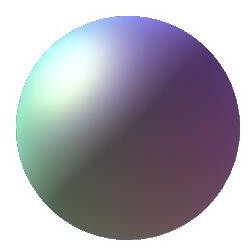
\includegraphics[scale=0.3]{../images/sphere.jpg}};
   \draw[black] ( 0,-2) node {Sphere};
   \draw ( 5, 0) node {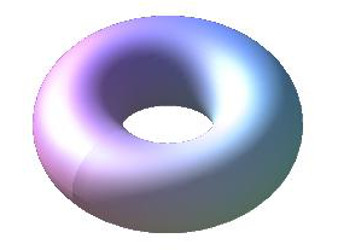
\includegraphics[scale=0.3]{../images/torus.jpg}};
   \draw[black] ( 5,-2) node {Torus};
   \draw (10, 0) node {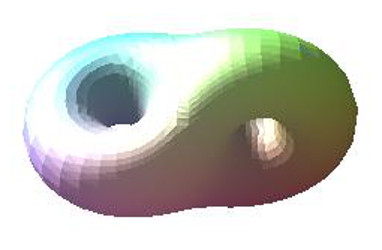
\includegraphics[scale=0.3]{../images/genus2.jpg}};
   \draw[black] (10,-2) node {Double torus};
  \end{scope}
  \begin{scope}[yshift=-4.5cm]
   \draw ( 0, 0) node {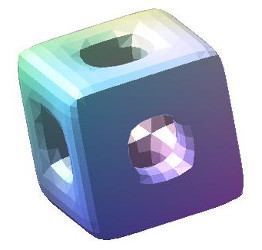
\includegraphics[scale=0.3]{../images/holycube.jpg}};
   \draw[black] ( 0,-2) node {Cube with holes};
   \draw ( 5, 0) node {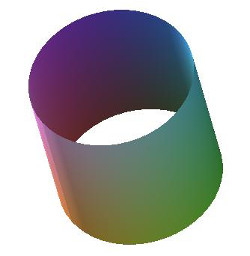
\includegraphics[scale=0.3]{../images/cyl.jpg}};
   \draw[black] ( 5,-2) node {Cylinder};
   \draw (10, 0) node {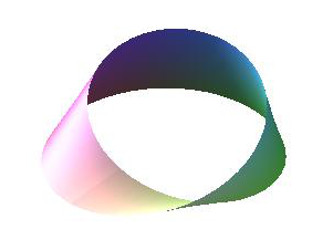
\includegraphics[scale=0.3]{../images/strip.jpg}};
   \draw[black] (10,-2) node {M\"obius strip};   
  \end{scope}
  \begin{scope}[yshift=-9.0cm]
   \draw ( 0, 0) node {
\includegraphics[scale=0.3]{../images/nonmanifold.jpg}};
   \draw[black] ( 0,-2) node {Two squares};
   \draw ( 5, 0) node {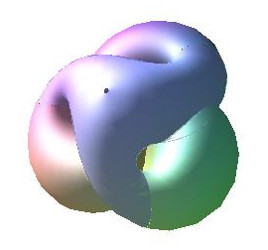
\includegraphics[scale=0.3]{../images/boys.jpg}};
   \draw[black] ( 5,-2) node {Boy's space};
   \draw (10, 0) node {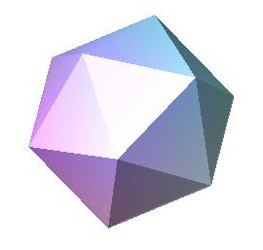
\includegraphics[scale=0.3]{../images/icos.jpg}};
   \draw[black] (10,-2) node {Icosahedron};   
  \end{scope}
 \end{tikzpicture}
\end{center}

The first key feature of these sets is that they have the following
property.
\begin{definition}\label{defn-compact}
 A subset $X\sse\R^n$ is \emph{compact} if 
 \begin{itemize}
  \item[(a)] There is a finite radius $r$ such that for all $x\in X$
   we have $\|x\|\leq r$.
  \item[(b)] For any convergent sequence $x_k\to a$ in $\R^n$, if all
   the terms $x_k$ lie in $X$, then the limit point $a$ also lies in
   $X$.  
 \end{itemize}
\end{definition}

\begin{example}
 The set $(0,5)\subset\R$ is not compact.  It has property~(a) (with
 $r=5$) but not property~(b), because there is a convergent sequence
 $1/n\to 0$ where all the terms $1/n$ lie in $(0,5)$ but the limit
 point does not lie in $(0,5)$.  However, the set $[0,5]$ is compact.
\end{example}

\begin{example}
 The subset $\Z^n\sse\R^n$ is not compact; it satisfies property~(b)
 but not property~(a).
\end{example}

\begin{remark}
 As many of you will know, Definition~\ref{defn-compact} is not the
 official definition of compactness; instead, it is a nontrivial theorem
 that Definition~\ref{defn-compact} is equivalent to the official
 definition of compactness.  However, this distinction will be
 harmless for us.
\end{remark}

\begin{remark}
 It is standard to say that a set $X$ is \emph{bounded} if it has
 property~(a), and \emph{closed} if it has property~(b), and you will
 need to be aware of this if you read other books.  However, we will
 not emphasise this terminology, as it can create confusion with the
 terms \emph{boundary} and \emph{closed surface} which we will
 introduce shortly.
\end{remark}

In the first half of this course we noted that there are things that
are like knots but which have infinitely many loops, and we decided to
exclude them from consideration.  For similar reasons, we will study
only compact surfaces.  

This resolves an ambiguity about our picture of the cylinder: are the
two end circles part of the picture or not?  In other words, which of
the following two sets are we looking at?
\begin{align*}
 C      &= \{(\cos(u),\sin(u),v) \st u,v\in\R,\; -1<v<1\} \\
 \ov{C} &= \{(\cos(u),\sin(u),v) \st u,v\in\R,\; -1\leq v\leq 1\},
\end{align*}
It is not hard to see that $\ov{C}$ is compact, but $C$ is not.  Thus,
we will define the cylinder to be $\ov{C}$ rather than $C$, so the
ends are included.  Similarly, the edge of the M\"obius strip will be
regarded as part of the strip, to ensure that the strip is a compact
set. 

The second key feature of the sphere and the torus is as follows: near any
point, we can cut out a small piece which can be identified with a
disc.  The double torus and the cube with holes have the same
property.  
\begin{center}
 \begin{tikzpicture}
  \draw[white] (0, 2) -- (10, 2);
  \draw[white] (0,-2) -- (10,-2);
  \begin{scope}
   \draw ( 0, 0) node {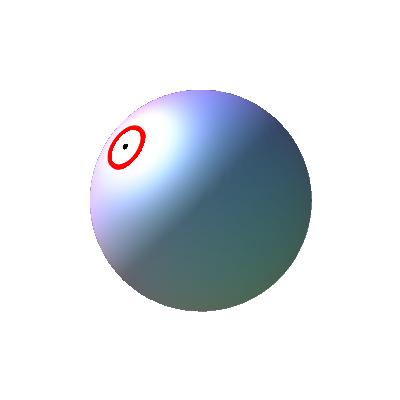
\includegraphics[scale=0.3]{../images/sphere_with_disc.jpg}};
   \draw ( 5, 0) node {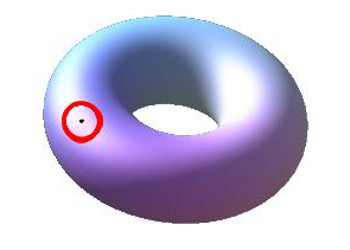
\includegraphics[scale=0.3]{../images/torus_with_disc.jpg}};
   \draw (10, 0) node {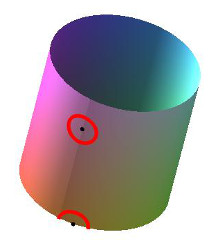
\includegraphics[scale=0.3]{../images/cyl_with_disc.jpg}};
  \end{scope}
 \end{tikzpicture}
\end{center}

\begin{predefinition}
 A \emph{closed surface} is a compact subset $X\sse\R^n$ for some $n$
 with the above property: any point has a neighbourhood which is a
 disc. 
\end{predefinition}

Later we will give a more careful version.

Note that the cylinder is \emph{not} a closed surface.  Instead, it
satisfies the following (as should be clear from the above picture):

\begin{predefinition}
 A \emph{surface with boundary} is a compact subset $X\sse\R^n$ for
 some $n$ such that any point $x\in X$ has a neighbourhood which is
 either a disc or a half-disc.  We say that $x$ is a \emph{boundary
  point} if it does not have a disc neighbourhood, but only a
 half-disc neighbourhood.  We write $\partial X$ for the set of
 boundary points.  
\end{predefinition}

The M\"obius strip is also a surface with boundary.  On the other
hand, if we take the union of two squares as in our earlier picture,
then points on the intersection line will not have a disc
neighbourhood or a half-disc neighbourhood, so the union is not a
closed surface or a surface with boundary.  Similarly, there are
points in Boy's space where a small neighbourhood looks like a pair of
intersecting squares, so Boy's space is also not a closed surface.
(For this reason we have avoided calling it Boy's surface, which is
the more traditional name.)  However, this space is closely related to
a closed surface called $\R P^2$ (the real projective plane), as we
now explain. 

We will use the following definition for $\R P^2$:
\[ \R P^2 = \{A\in M_3(\R)\st \text{trace}(A)=1,\; A^2=A^T=A\}. \]
A $3\times 3$ matrix has $9$ entries, so we can identify $M_3(\R)$
with $\R^9$, and so identify $\R P^2$ with a subspace of $\R^9$.  It
turns out that this is a closed surface.  We will only sketch the
first step in the proof of this fact.  Recall that the unit sphere can
be described as
\[ S^2 = \{(x=(x_1,x_2,x_3)\in \R^3 \st \sum_ix_i^2 = 1\}. \]
\begin{lemma}\label{lem-proj-plane}
 There is a continuous surjective map $q\:S^2\to\R P^2$ such that
 $q(x)=q(y)$ iff $x=\pm y$.  In other words, $\R P^2$ can be obtained
 from $S^2$ by identifying $x$ with $-x$ for all $x$.
\end{lemma}
\begin{proof}
 Given any $x\in S^2$, we define a matrix $q(x)\in M_3(\R)$ by
 $q(x)_{ij}=x_ix_j$.  We then have
 \begin{align*}
  \text{trace}(q(x)) &= \sum_i q(x)_{ii} = \sum_i x_i^2 = 1 \\
  (q(x)^T)_{ij} &= q(x)_{ji} = x_jx_i = q(x)_{ij} \\
  (q(x)^2)_{ik} &= \sum_k q(x)_{ij}q(x)_{jk}
   = x_i x_k \sum_j x_j^2 = x_ix_k = q(x)_{ik},
 \end{align*}
 so $q(x)\in\R P^2$.  In the opposite direction, suppose that
 $A\in\R P^2$, and put $L=\{x\st Ax=x\}$ and $Z=\{x\st Ax=0\}$.  Using
 $A^2=A$ one can check that $\R^3=L\oplus Z$.  One can then choose a
 basis for $L$ and a basis for $Z$, and by writing $A$ in terms of
 these bases we find that $\text{trace}(A)=\dim(L)$.  By assumption we
 have $\text{trace}(A)=1$, so $L$ is a line, so it contains precisely
 two unit vectors, say $x$ and $-x$.  With a little more linear
 algebra (and using the additional property $A^T=A$), one can check
 that $A=q(x)=q(-x)$, and that $x$ and $-x$ are the only vectors with
 this property.  Thus, we see that $q\:S^2\to\R P^2$ is surjective,
 and we have $q(x)=q(y)$ iff $x=\pm y$. 
\end{proof}
Now if $U$ is a small disc in $S^2$, then $-U$ will be
another small disc that does not overlap with $-U$, and $q(U)$ will be
a small disc in $\R P^2$.  By analysing this situation a little more
carefully, one can check that $\R P^2$ is indeed a closed surface.

However, it turns out that it is not possible to make a copy of 
the space $\R P^2\sse\R^9$ in $\R^3$.  One can make a copy in $\R^4$,
but if you try to do it in $\R^3$, then the resulting surface will
intersect itself.  There is a map $f\:\R P^2\to \R^3$ such that 
$f(\R P^2)$ is Boy's space, so Boy's space is almost a copy of 
$\R P^2$, but this is not quite right, because $f$ fails to be
injective in some places.

This is analogous to the fact that the trefoil (or any other
interesting knot) cannot be represented in $\R^2$ without
self-intersections.  

The fact that $\R P^2$ cannot be embedded in $\R^3$ is closely related
to the fact that $\R P^2$ is not orientable.  We will explain what
this means in the simpler case of the M\"obius strip.  
\[ \begin{array}{ccc}
    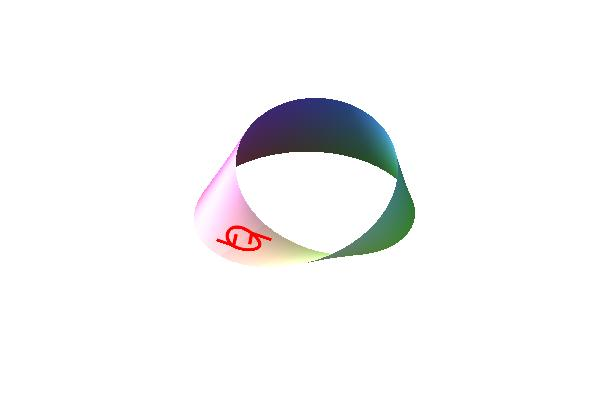
\includegraphics[scale=0.45,trim=5cm 2cm 5cm 2cm,clip]{../images/mobius0.jpg} &
    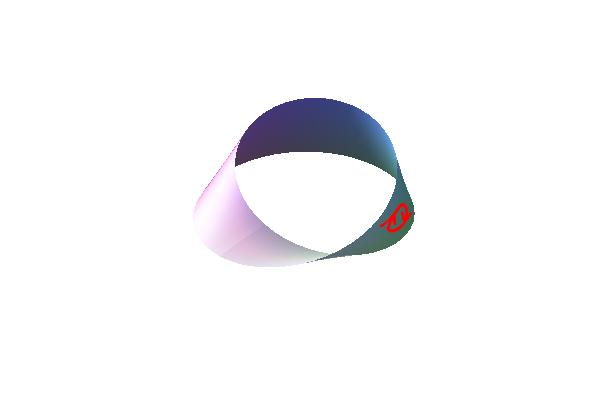
\includegraphics[scale=0.45,trim=5cm 2cm 5cm 2cm,clip]{../images/mobius1.jpg} &
    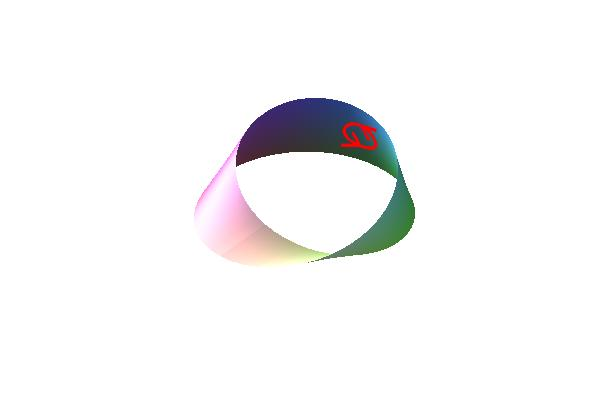
\includegraphics[scale=0.45,trim=5cm 2cm 5cm 2cm,clip]{../images/mobius2.jpg} \\
    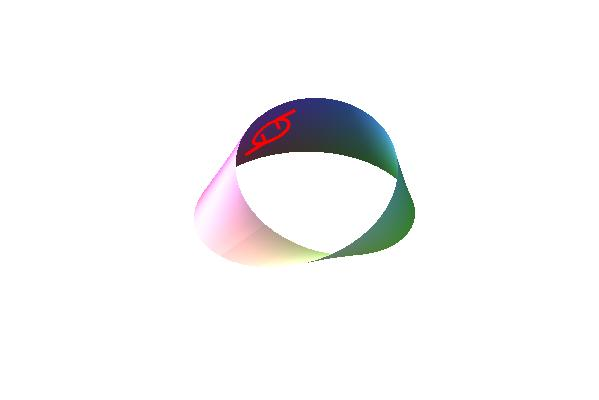
\includegraphics[scale=0.45,trim=5cm 2cm 5cm 2cm,clip]{../images/mobius3.jpg} &
    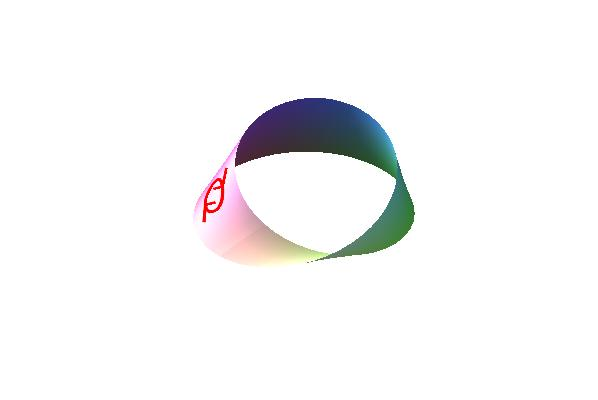
\includegraphics[scale=0.45,trim=5cm 2cm 5cm 2cm,clip]{../images/mobius4.jpg} &
    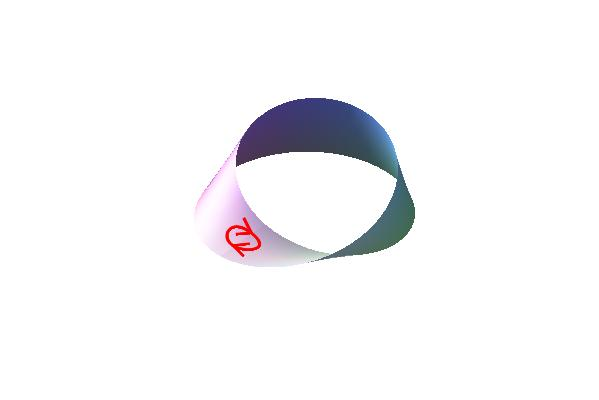
\includegraphics[scale=0.45,trim=5cm 2cm 5cm 2cm,clip]{../images/mobius5.jpg}
   \end{array}
\]
We can take a circle marked with arrows circulating anticlockwise and
slide it around the strip.  When we have slid it around once, the
arrows end up circulating clockwise.  If we go around a second time,
then they end up anticlockwise again.  This is not possible with the
sphere or the torus or any other closed surface embedded in $\R^3$;
for those surfaces, there is a consistent definition of clockwise and
anticlockwise, and we cannot convert a clockwise circle to an
anticlockwise circle by sliding it around.

We will eventually be able to classify both orientable and
nonorientable surfaces, but many things work differently in the two
cases.

\section{Connected sums}
\label{sec-connected-sum}

Let $X$ and $Y$ be connected surfaces, possibly with boundary.  We can
make a new surface $X\# Y$ (called the \emph{connected sum} of $X$ and
$Y$) as follows.  First, we let $2D$ denote the disc of radius $2$
centred at the origin in $\R^2$, and choose a continuous embedding
$i\:2D\to X$.  Recall that $D'$ is the open disc of radius one, and
remove $i(D')$ from $X$ to get a new space $X^*=X\sm i(D')$.  Note
that we still have a circle $i(S^1)\subset X^*$, which forms part (or
maybe all) of the boundary of $X^*$.  Similarly, we choose an
embedding $j\:2D\to Y$, and put $Y^*=Y\sm j(D')$.  We again have a
circle $j(S^1)\sse Y^*$.  We let $X\# Y$ denote the space formed from
$X^*$ and $Y^*$ by attaching $i(x,y)$ to $j(x,-y)$ for all 
$(x,y)\in S^1$. 

\begin{proposition}\label{prop-sum-surface}
 The space $X\# Y$ is again a surface (possibly with boundary).  
\end{proposition}
\begin{proof}
 Inside $X\# Y$ we have a circle $C$ where $X^*$ and $Y^*$ are joined
 together.  Consider a point $u$ that does not lie on $C$.  If $u$
 lies in $X^*\sm i(S^1)$, then we can choose a disc or half-disc
 neighbourhood $U$ of $u$ in $X$, and provided we take $U$ to be small
 enough, it will be contained in $X^*\sm i(S^1)$.  Thus, this will
 give a disc or half-disc neighbourhood of $u$ in $X\# Y$.  The same
 argument works if $u$ lies in $Y^*\sm j(S^1)$.  This just leaves the
 case of a point $u\in C$.  Put 
 \[ A=2D'\sm D'=\{(x,y)\in\R^2 \st 1\leq \|(x,y)\| < 2\}, \]
 so we have an subset $i(A)$ in $X^*$ and an open subset $j(A)$ in
 $Y^*$.  Together, these give an open subset of $X\# Y$, which
 consists of two copies of $A$ glued together along a circle.  To see
 the effect of this, put 
 \begin{align*}
  A' &= \{(x,y)\in\R^2\st 1/2 < \|(x,y)\| \leq 1\} \\
  B  &=  A\cup A' = \{(x,y)\in\R^2\st 1/2 < \|(x,y)\| < 2\}.
 \end{align*}
 There is a homeomorphism $A\to A'$ given by 
 \[ (x,y)\mapsto(x/(x^2+y^2),-y/(x^2+y^2)). \]
 (If we identify $\R^2$ with $\C$, this is just $z\mapsto 1/z$.)  On
 $S^1$, this is just $(x,y)\mapsto(x,-y)$, which is the rule we used
 when identifying $i(S^1)$ with $j(S^1)$.  Thus, the set
 $U=i(A)\cup j(A)$ can be identfied with $A\cup A'=B$.  From this it
 follows that every point in $U$ has a full disc neighbourhood in $U$,
 which completes the proof that $X\# Y$ is a surface. 
\end{proof}

\begin{remark}\label{rem-sum-well-defined}
 The notation $X\# Y$ suggests that we get a well-defined result,
 independent of the choice of embeddings $i$ and $j$.  This is in fact
 true, but we will not prove it.
\end{remark}

The most basic case is as follows:
\begin{proposition}
 For any surface $X$, we have $X\# S^2\simeq X$.
\end{proposition}
\begin{proof}
 Note that $(S^2)^*$ is obtained from $S^2$ by removing an open disc,
 which we can choose to be the upper hemisphere.  That means that
 $(S^2)^*$ is the (closed) lower hemisphere, which is again a disc.
 We form $X^*$ by removing a disc from $X$, but we just replace that
 disc when we attach $(S^2)^*$ to form $X\# S^2$, so $X\# S^2=X$.
\end{proof}

Another basic case is as follows:
\begin{proposition}
 For any surface $X$, the surface $X\# D$ is homeomorphic to $X^*$
 (the space obtained by removing a disc from $X$).
\end{proposition}
\begin{proof}
 Note that $D^*$ is just $D\sm D'$, where $D'$ is a smaller open disc
 nested in $D$.  To form $X\# D$ we first remove a disc from $X$, then
 we attach $D\sm D'$.  The overall effect is the same as just removing
 a copy of $D'$ from $X$, which is again $X^*$.
\end{proof}

If we let $T$ denote the torus, then $T\# T$ is as follows:
\[ 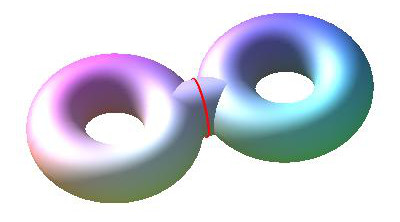
\includegraphics[scale=0.5]{../images/double_torus.jpg} \]
The left half is one copy of $T^*$, the right half is the other copy,
and they are joined along the circle shown in red.  Similarly, the
surface $T^{\# 3}=T\# T\# T$ looks like this:
\[ 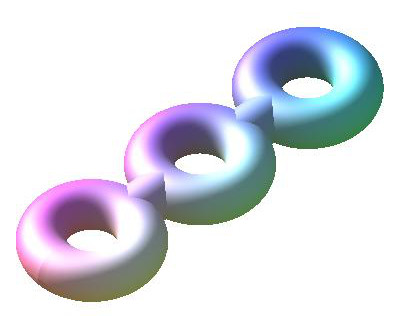
\includegraphics[scale=0.5]{../images/triple_torus.jpg} \]
We will show later that every closed, connected orientable surface is
homeomorphic to $T^{\# n}$ for some $n\geq 0$.

\section{Formal definitions}
\label{sec-surf-formal}

We next give a more rigorous version of the definitions in
Section~\ref{sec-surf-intro}.  Most of this should be revision for
most students, so we will be brief.

Surfaces are modelled on discs, defined as follows.

\begin{definition}
 We put 
 \begin{align*}
  D   &= \{(x,y)\in\R^2\st x^2+y^2 \leq 1\} 
       = \text{ the closed unit disc } \\
  D' &= \{(x,y)\in\R^2\st x^2+y^2 < 1\} 
       = \text{ the open unit disc } \\
  D'_+ &= \{(x,y)\in D'\st y\geq 0\} 
       = \text{ the standard open half-disc }.
 \end{align*}
\end{definition}

In a closed surface, every point should have a neighbourhood which can
be identified with $D'$.  We next give a formal definition for the kind
of identification that we need to consider.

\begin{definition}
 We recall that the standard definition of continuity works perfectly
 well for maps between subsets of $\R^d$: if $X\sse\R^n$ and
 $Y\sse\R^m$ and $f\:X\to Y$, we say that $f$ is \emph{continuous} if 
 for every convergent sequence $x_k\to a$ with all $x_k$ and $a$ in
 $X$, the sequence $f(x_k)$ converges to $f(a)$.  We say that $f$ is a
 \emph{homeomorphism} if it is a bijection, and both $f\:X\to Y$ and
 $f^{-1}\:Y\to X$ are continuous.  We say that $X$ and $Y$ are
 \emph{homeomorphic} if there exists a homeomorphism from $X$ to $Y$.
\end{definition}

We next need a definition of ``neighbourhood''.
\begin{definition}
 Ler $x$ be a point in $\R^n$, and let $\ep$ be a positive real
 number.  We then put 
 \[ B_\ep(x) = \{y\in\R^n\st \|x-y\|<\ep\}. \]
 This is called the \emph{open ball of radius $\ep$ around $x$}.
\end{definition}

\begin{definition}
 Let $X$ be a subset of $\R^n$, and consider a set $U\sse X$.  We say
 that $U$ is \emph{open in $X$} if for each $x\in X$ there exists
 $\ep>0$ such that $X\cap B_{\ep}(x)\sse U$.

 An \emph{open neighbourhood} of a point $a\in X$ is a set $U\sse X$
 such that $U$ is open in $X$ and $a\in U$.
\end{definition}

\begin{definition}\leavevmode
 \begin{itemize}
  \item[(a)] A \emph{closed surface} is a compact subset
   $X\subset\R^n$ (for some $n$) such that every point $a\in X$ has an
   open neighbourhood that is homeomorphic to $D'$.
  \item[(b)] A \emph{surface with boundary} is a compact subset
   $X\subset\R^n$ (for some $n$) such that every point $a\in X$ has an
   open neighbourhood that is either homeomorphic to $D'$ or
   homeomorphic to $D'_+$.
 \end{itemize}
\end{definition}

\begin{definition}
 Let $X$ be a closed surface.  A \emph{disconnection} of $X$ is a pair
 of subsets $Y,Z\sse X$ such that 
 \begin{itemize}
  \item $Y$ is itself a closed surface, and so is $Z$
  \item $Y\cup Z=X$ and $Y\cap Z=\emptyset$
  \item Neither $Y$ nor $Z$ s empty.
 \end{itemize}
 We say that $X$ is \emph{connected} if no such disconnection exists.
\end{definition}

We will mostly be interested in connected surfaces.

\section{Piecewise linear versions}
\label{sec-surf-pl}

In practice, we will mostly work with piecewise linear surfaces, which
we now introduce.  

\begin{definition}
 Let $a_1,a_2$ and $a_3$ be vectors in $\R^n$.  We say that they are
 in \emph{general position} if the vectors $a_2-a_1$ and $a_3-a_1$ are
 linearly independent, so there is no line that contains all three
 points.  If so, we put
 \[ \Delta(a_1,a_2,a_3) = \{t_1a_1+t_2a_2+t_3a_3\st 
     t_1,t_2,t_3\geq 0,\; t_1+t_2+t_3=1\}.
 \]
 This is a triangle in $\R^n$ with vertices $a_i$.  The three edges
 are 
 \begin{align*}
  E_1 &= \{t_2a_2+t_3a_3\st t_2,t_3\geq 0,\; t_2+t_3=1\} \\
  E_2 &= \{t_1a_1+t_3a_3\st t_1,t_3\geq 0,\; t_1+t_3=1\} \\
  E_3 &= \{t_1a_1+t_2a_2\st t_1,t_2\geq 0,\; t_1+t_2=1\}.
 \end{align*}
\end{definition}

\begin{definition}\label{defn-triangulation}
 Let $X$ be a subset of $\R^n$.  A \emph{linear surface triangulation}
 of $X$ is a list of triangles $T_1,\dotsc,T_N$ as above, such that
 \begin{itemize}
  \item[(a)] For each $i\neq j$, the intersection $T_i\cap T_j$ is either 
   empty; or a single point which is a vertex of $T_i$ and also a
   vertex of $T_j$; or a line segment which is an edge of $T_i$ and
   also an edge of $T_j$.
  \item[(b)] For each triangle $T_i$ and each edge $E\subset T_i$, there is
   at most one other triangle $T_j$ such that $E$ is also an edge of
   $T_j$.  (We say that $E$ is an \emph{interior edge} if there exists
   a triangle $T_j$ as above; otherwise we say that $E$ is a
   \emph{boundary edge}.)
  \item[(c)] For any vertex $V$ in $X$, the set of triangles containing
   $V$ can be listed as $T_{i_1},\dotsc,T_{i_m}$ in such a way
   that $T_{i_k}$ shares an edge with $T_{i_{k+1}}$, and $T_{i_m}$
   may or may not share an edge with $T_{i_1}$, and there are no other
   common edges.  (We say that $V$ is an \emph{interior vertex} if
   $T_{i_m}$ shares an edge with $T_{i_1}$; otherwise we say that $V$
   is a \emph{boundary vertex}.)
 \end{itemize}
 We say that a linear surface triangulation is \emph{closed} if there
 are no boundary edges (and therefore no boundary vertices.)

 A \emph{piecewise-linear surface with boundary} is a subset
 $X\sse\R^n$ for which there exists a linear surface triangulation.  A
 \emph{piecewise-linear closed surface} is a subset for which there
 exists a closed linear surface triangulation.
\end{definition}

\begin{example}
 Let $X$ be the surface of a cube.  This consists of six squares.  We
 can draw a diagonal line across each square to divide it into two
 triangles.  The resulting twelve triangles give a linear surface
 triangulation of $X$.  

 \begin{center}
  \begin{tikzpicture}[scale=3]
   \fill[   cyan!30] (0,0) -- (1,0) -- (0,1);
   \fill[   blue!30] (0,1) -- (1,1) -- (1,0);
   \fill[    red!30] ( 0.0,0.0) -- (-0.3, 0.4) -- ( 0.0, 1.0);
   \fill[ orange!30] (-0.3,0.4) -- (-0.3, 1.4) -- ( 0.0, 1.0);
   \fill[  green!30] ( 0.0,1.0) -- ( 1.0, 1.0) -- ( 0.7, 1.4);
   \fill[magenta!30] ( 0.0,1.0) -- (-0.3, 1.4) -- ( 0.7, 1.4);
   \draw[gray] (0,0) -- (1,0) -- (1,1) -- (0.7,1.4) -- (-0.3,1.4) -- (-0.3,0.4) -- (0,0);
   \draw[gray] (0,0) -- (0,1) -- (-0.3,1.4);
   \draw[gray] (0,1) -- (1,1);
   \draw[thin,gray] (-0.3,0.4) -- (0,1) -- (1,0);
   \draw[thin,gray] (0,1) -- (0.7,1.4);
   \fill[black] (0.0,0.4) circle(0.02);
   \fill[black] (0.7,0.7) circle(0.02);
   \fill[black] (0.0,1.0) circle(0.02);
   \begin{scope}[xshift= 0.80cm,yshift=0.7cm,scale=0.5] \draw[black](0,0) node {$a$}; \end{scope}
   \begin{scope}[xshift= 0.10cm,yshift=0.4cm,scale=0.5] \draw[black](0,0) node {$b$}; \end{scope}
   \begin{scope}[xshift=-0.10cm,yshift=1.0cm,scale=0.5] \draw[black](0,0) node {$c$}; \end{scope}
  \end{tikzpicture}
 \end{center}

 Each of the points $a$, $b$ and $c$ has a disc neighbourhood:
 \begin{center}
  \begin{tikzpicture}
   \begin{scope}
    \fill[blue!30] (0,0) circle(1);
    \fill[black] (0,0) circle(0.05);
    \draw[black] (0.3,0) node {\huge $a$};
   \end{scope}
   \begin{scope}[xshift=4cm]
    \fill[cyan!30] (0,0) -- (0,-1) arc(-90: 90:1) -- (0,0);
    \fill[ red!30] (0,0) -- (0, 1) arc( 90:270:1) -- (0,0);
    \fill[black] (0,0) circle(0.05);
    \draw[black] (0.3,0) node {\huge $b$};
   \end{scope}
   \begin{scope}[xshift=8cm]
    \fill[  green!30] (0,0) -- (  0:1) arc(  0: 60:1) -- (0,0);
    \fill[magenta!30] (0,0) -- ( 60:1) arc( 60:120:1) -- (0,0);
    \fill[ orange!30] (0,0) -- (120:1) arc(120:180:1) -- (0,0);
    \fill[    red!30] (0,0) -- (180:1) arc(180:240:1) -- (0,0);
    \fill[   cyan!30] (0,0) -- (240:1) arc(240:300:1) -- (0,0);
    \fill[   blue!30] (0,0) -- (300:1) arc(300:360:1) -- (0,0);
    \fill[black] (0,0) circle(0.05);
    \draw[black] (0.3,0) node {\huge $c$};
   \end{scope}
  \end{tikzpicture}
 \end{center}
\end{example}

It should be clear that the above construction works for any PL closed
surface.  Axiom~(a) says that the triangles do not interfere with each
other except on the boundary, so for any point in a triangle that is
not on an edge, a small piece of the triangle can be used as a disc
neighbourhood.  For a point on an edge that not a vertex, Axiom~(b)
says that there will be precisely two triangles that contain the
relevant edge, and we can take a half-disc from each of these
triangles to get a full disc neighbourhood of the point.  Finally,
Axiom~(c) is precisely what we need to get a disc neighbourhood  for
each vertex.  Thus, any PL closed surface is a closed surface, as the
name suggests.  Similarly, a PL surface with boundary is a surface
with boundary.

\begin{theorem}
 Let $X$ be any closed surface.  Then there is a PL closed surface $Y$
 such that $Y$ is homeomorphic to $X$.
\end{theorem}

The proof of this theorem is quite hard, and we will not discuss it.
However, it is reasonably easy to see that it is true in specific
cases.  In fact, if you look closely at the computer pictures of
smoothly curved surfaces, you will see that the computer has actually
used triangles, and has drawn a PL surface which is a close
approximation to the surface we first considered.

For the rest of this course, we will work with PL closed surfaces.

\section{Surface words}
\label{sec-surf-words}

Our main aim is to classify surfaces up to homeomorphism.  The first
step is to introduce surface words, which are a kind of combinatorial
recipe for building surfaces by starting with a disc and gluing
together certain parts of the boundary.  We will show that every
connected surface can be obtained in this way, if we choose a suitable
surface word.  Our first choice of surface word may be very
complicated, but we will also show that the word can be simplified in
various ways, without changing the corresponding surface.  (This is
loosely analogous to simplifying knot diagrams by Reidemeister moves.) 

\begin{definition}\label{defn-word}
 A \emph{surface word} is a sequence of barred or unbarred latters, in
 which each letter (ignoring bars) occurs at most twice.  Such a word
 is \emph{closed} if every letter occurs precisely twice.  It is
 \emph{nonorientable} if there is a letter which occurs twice without
 a bar or twice with a bar; otherwise it is \emph{orientable}.
\end{definition}

\begin{remark}\label{rem-double-bar}
 In various places we will refer to $\xb$, where $x$ might already be
 a barred letter.  This should be interpreted by the rule
 $\ov{\ov{a}}=a$.  
\end{remark}

\begin{example}\label{eg-standard-words}\leavevmode
 \begin{itemize}
  \item The \emph{sphere word} $S$ is the empty word, with no letters.
  \item The \emph{torus word} is $T=xy\xb\,\yb$.
  \item The \emph{projective plane word} is $P=xx$.
  \item The \emph{Klein bottle word} is $K=xy\xb\,y$.
  \item The \emph{disc word} is $D=x$.
  \item The \emph{cylinder word} is $C=xy\xb\,z$.
  \item The \emph{M\"obius word} is $M=xyxz$.
 \end{itemize}
 Note that 
 \begin{itemize}
  \item $S$, $T$, $P$ and $K$ are closed, but the others are not.
  \item $S$, $T$, $C$ and $D$ are orientable, but the others are not.
 \end{itemize}
\end{example}

\begin{example}\label{eg-non-word}
 The sequence $xy\xb\,\yb\,x$ is not a surface word, because $x$ occurs
 three times (once barred and twice unbarred).
\end{example}

\begin{definition}\label{defn-Sigma-W}
 Given a surface word $W$, we construct a space $\Sg(W)$ as follows.
 Let $n$ be the number of letters in $W$.  If $n=0$ (so $W$ is the
 empty word) we define $\Sg(W)$ to be the sphere $S^2$.  Otherwise, we
 take the disc 
 \[ D = \{(x,y)\in\R^2\st x^2+y^2\leq 1\}, \]
 and we divide the boundary circle into $n$ equal arcs 
 \[ A_k =
     \{(\cos(\tht),\sin(\tht))\st k-1\leq \frac{n\tht}{2\pi}\leq k\}
 \]
 for $1\leq k\leq n$.  We then define $\Sg(W)$ to be the space
 obtained by identifying $A_j$ with $A_k$ whenever the $j$'th and
 $k$'th letters in $W$ are the same.  More precisely, if the $j$'th
 and $k$'th letters are the same and both are barred or both are
 unbarred, then we identify $A_j$ with $A_k$ in the same direction,
 but if one of the letters has a bar and the other does not, then we
 identify $A_j$ with $A_k$ in the opposite direction.
\end{definition}

\begin{remark}\label{rem-polygon}
 It is often more convenient to draw a polygon with $n$ straight
 sides, instead of a disc with $n$ curved arcs.  This is fine as long
 as $n\geq 3$.  
\end{remark}

\begin{example}\label{eg-cylinder-word}
 Consider the cylinder word $C=xy\xb,z$.  We can draw $\Sg(C)$ as shown
 on the left below.
 \begin{center}
  \begin{tikzpicture}
   \begin{scope}
    \filldraw[fill=blue!30,draw=black] (0,0) circle(2);
    \draw (  0:1.9) -- (  0:2.1);
    \draw ( 90:1.9) -- ( 90:2.1);
    \draw (180:1.9) -- (180:2.1);
    \draw (270:1.9) -- (270:2.1);
    \draw[black] ( 45:1.70) node {$A_1$};
    \draw[black] (135:1.70) node {$A_2$};
    \draw[black] (225:1.70) node {$A_3$};
    \draw[black] (315:1.70) node {$A_4$};
    \draw[black] ( 45:2.30) node {$x$};
    \draw[black] (135:2.30) node {$y$};
    \draw[black] (225:2.30) node {$\xb$};
    \draw[black] (315:2.30) node {$z$};
   \end{scope}
   \begin{scope}[xshift=6cm]
    \filldraw[fill=blue!30,draw=black] (-1.7,-1.7) rectangle (1.7,1.7);
    \draw[black,->] ( 1.7,-1.7) -- ( 1.7, 0.0);    
    \draw[black,->] (-1.7,-1.7) -- (-1.7, 0.0);    
    \draw[black,->] ( 1.7, 1.7) -- ( 0.0, 1.7);    
    \draw[black,->] (-1.7,-1.7) -- ( 0.0,-1.7);
    \draw[black] ( 2.0, 0.0) node {$x$};    
    \draw[black] (-2.0, 0.0) node {$\xb$};
    \draw[black] ( 0.0, 2.0) node {$y$};
    \draw[black] ( 0.0,-2.0) node {$z$};
   \end{scope}
   \begin{scope}[xshift=11cm]
    \draw (0,0) node{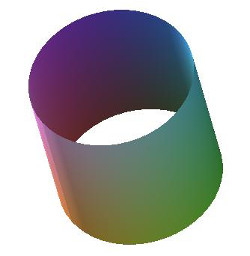
\includegraphics[scale=0.45]{../images/cyl.jpg}};
   \end{scope}
  \end{tikzpicture}
 \end{center}
 The arcs $A_1$ and $A_3$ are labelled $x$ and $\ov{x}$, so they are
 glued with reversed directions.  It is easier to see the effect of this if
 we redraw the picture as shown in the middle.  There, we have rotated
 the picture and straightened the sides to make a square.  Each arc
 with an unbarred letter has been given an anticlockwise arrow, and 
 each arc with a barred letter has been given a clockwise arrow.  The
 rule is now that sides with matching labels get glued in the
 direction indicated by the arrows.  Attaching the two $x$'s together
 gives a cylinder.  Thus, $\Sg(C)$ is a cylinder, which justifies the
 name ``cylinder word'' for $C$.
\end{example}

\begin{example}\label{eg-torus-word}
 For the torus word $T=xy\xb\,\yb$, we have the following picture.
 \begin{center}
  \begin{tikzpicture}
   \begin{scope}
    \filldraw[fill=blue!30,draw=black] (-1.7,-1.7) rectangle (1.7,1.7);
    \draw[black,->] ( 1.7,-1.7) -- ( 1.7, 0.0);    
    \draw[black,->] (-1.7,-1.7) -- (-1.7, 0.0);    
    \draw[black,->] ( 1.7, 1.7) -- ( 0.0, 1.7);    
    \draw[black,->] ( 1.7,-1.7) -- ( 0.0,-1.7);
    \draw[black] ( 2.0, 0.0) node {$x$};    
    \draw[black] (-2.0, 0.0) node {$\xb$};
    \draw[black] ( 0.0, 2.0) node {$y$};
    \draw[black] ( 0.0,-2.0) node {$\yb$};
   \end{scope}
   \begin{scope}[xshift=7cm]
    \draw (0,0) node{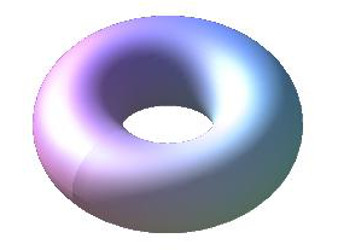
\includegraphics[scale=0.45]{../images/torus.jpg}};
   \end{scope}
  \end{tikzpicture}
 \end{center}
 Attaching the two $x$'s together gives a cylinder.  The two edges
 marked $y$ become the top and bottom circles of the cylinder, and
 when we glue them together we get a torus.  Thus, $\Sg(T)$ is a
 torus, which justifies the name ``torus word'' for $T$.
\end{example}

\begin{example}\label{eg-mobius-word}
 For the M\"obius word $M=xyxz$, it is convenient to stretch the
 picture horizontally:
 \begin{center}
  \begin{tikzpicture}
   \draw[white] (0,-2.2) -- (0,2.2);
   \begin{scope}
    \filldraw[fill=blue!30,draw=black] (-3.7,-0.7) rectangle (3.7,0.7);
    \draw[black,->] ( 3.7,-0.7) -- ( 3.7, 0.0);    
    \draw[black,->] (-3.7, 0.7) -- (-3.7, 0.0);    
    \draw[black,->] ( 1.7, 0.7) -- ( 0.0, 0.7);    
    \draw[black,->] (-1.7,-0.7) -- ( 0.0,-0.7);
    \draw[black] ( 4.0, 0.0) node {$x$};    
    \draw[black] (-4.0, 0.0) node {$x$};
    \draw[black] ( 0.0, 1.0) node {$y$};
    \draw[black] ( 0.0,-1.0) node {$z$};
   \end{scope}
   \begin{scope}[xshift=8cm]
    \draw (0,0) node{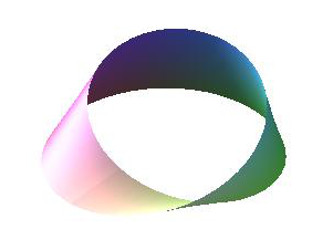
\includegraphics[scale=0.45]{../images/strip.jpg}};
   \end{scope}
  \end{tikzpicture}
 \end{center}
 Here we need to twist the strip before connecting the ends together,
 in order to make the arrows match up.  This gives a M\"obius band.
\end{example}

\begin{example}\label{eg-sphere-word}
 For the sphere word $S$, the space $\Sg(S)$ is a sphere by
 definition.  For the disc word $D=x$, the space $\Sg(D)$ consists of
 a disc with a single boundary arc $A_1$ and no gluing (because there
 are no repeated letters in the word).  In other words, $\Sg(D)$ is a
 disc.  
\end{example}

\begin{example}\label{eg-pplane-word}
 Now consider the projective plane $\R P^2$.  If $a\in\R P^2$, we can
 choose a point $u\in S^2\subset\R^3$ with $q(u)=q(-u)=a$.  If the
 $z$-coordinate of $u$ is negative then we put $v=-u$, otherwise we
 put $v=u$.  We now have a point $v$ in the upper hemisphere $S^2_+$
 of $S^2$ such that $q(v)=a$.  If $v$ does not lie on the equator,
 then $v$ is the \emph{only} point in $S^2_+$ such that $q(v)=a$.
 However, if $v$ lies on the equator, then $-v$ also lies on the
 equator, and $q(-v)=q(v)$.  This means that $\R P^2$ can be obtained
 from $S^2_+$ by identifying $v$ with $-v$ whenever $v$ lies on the
 equator.  

 Note also that $S^2_+$ can be identified with the closed disc
 $D$ by the map $(x,y)\mapsto(x,y,\sqrt{1-x^2-y^2})$.  The
 equator corresponds to the boundary circle $S^1\subset D$,
 consisting of points $v=(\cos(\tht),\sin(\tht))$.  In this picture,
 we have
 \[ -v = (-\cos(\tht),-\sin(\tht)) = (\cos(\pi+\tht),\sin(\pi+\tht)).
 \]
 Thus, if we divide $S^1$ into two arcs
 \begin{align*}
  A_1 &= \{(\cos(\tht),\sin(\tht))\st 0\leq\tht\leq\pi\} \\
  A_2 &= \{(\cos(\tht),\sin(\tht))\st \pi\leq\tht\leq 2\pi\},
 \end{align*}
 then $A_1$ gets identified with $A_2$, with no change of direction.
 This means that $\R P^2\simeq \Sg(xx)=\Sg(P)$.
\end{example}

\begin{example}\label{eg-klein-word}
 The picture on the left shows the Klein bottle word $K=xy\xb\,y$.
 After identifying the two edges marked $x$, we have a cylinder.  We
 then need to identify the two end circles, but without reversing the
 orientation.  This cannot be done in $\R^3$ without
 self-intersections.  We need to pass one end of the cylinder through
 the wall of the cylinder, then we can connect the two ends together
 while preserving the direction of the arrows.  
 \begin{center}
  \begin{tikzpicture}
   \draw[white] (0,2.5) -- (1,2.5);
   \begin{scope}
    \filldraw[fill=blue!30,draw=black] (-1.7,-1.7) rectangle (1.7,1.7);
    \draw[black,->] ( 1.7,-1.7) -- ( 1.7, 0.0);    
    \draw[black,->] (-1.7,-1.7) -- (-1.7, 0.0);    
    \draw[black,->] ( 1.7, 1.7) -- ( 0.0, 1.7);    
    \draw[black,->] (-1.7,-1.7) -- ( 0.0,-1.7);
    \draw[black] ( 2.0, 0.0) node {$x$};    
    \draw[black] (-2.0, 0.0) node {$\xb$};
    \draw[black] ( 0.0, 2.0) node {$y$};
    \draw[black] ( 0.0,-2.0) node {$y$};
   \end{scope}

   \begin{scope}[xshift=7cm]
    \draw (0,0) node {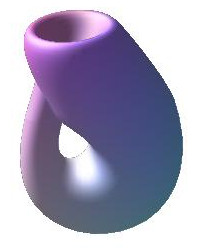
\includegraphics[scale=0.5]{../images/klein_bottle.jpg}};
   \end{scope}
  \end{tikzpicture}
 \end{center} 
 This gives a self-intersecting surface in $\R^3$, as shown on the
 right.  In higher dimensions we can perform the gluing without
 creating self-intersections; this gives a surface called the
 \emph{Klein bottle}.
\end{example}

\begin{lemma}\label{lem-Sg-embeds}
 For any surface word $W$, the space $\Sg(W)$ can be realised as a
 simplicial complex in $\R^N$ for some $N$.  
\end{lemma}
\begin{proof}
 The basic idea is to divide the disc up into triangles, and then
 embed each triangle linearly in $\R^N$.  If two arcs in the disc have
 the same label, then we should place the corresponding triangles in
 $\R^N$ in such a way that the relevant edges match up.  This will
 give us an embedding of $\Sg(W)$ in $\R^N$.

 However, the above process will not work if we use too few
 triangles.  To see this, consider the following subdivision of the
 square.  
 \begin{center}
  \begin{tikzpicture}
   \begin{scope}
    \draw[thin,black] (-2,-2) -- ( 2,-2) -- ( 2, 2) -- (-2, 2) -- cycle;
    \draw[thin,black] (-2,-2) -- ( 2, 2);
    \draw[thin,black] (-2, 2) -- ( 2,-2);
    \draw[thin,black] ( 0,-2) -- ( 0, 2);
    \draw[thin,black] (-2, 0) -- ( 2, 0);
    \fill[white] (0.01,0.01) rectangle (0.4,0.4);
    \draw[black] (0.2,0.2) node{$0$};
    \draw[black] ( 2, 2) node[anchor=south] {$1$};
    \draw[black] ( 0, 2) node[anchor=south] {$2$};
    \draw[black] (-2, 2) node[anchor=south] {$3$};
    \draw[black] ( 1, 1) node[anchor=north west] {$a$};
    \draw[black] ( 1, 2) node[anchor=south] {$b$};
    \draw[black] (-1, 2) node[anchor=south] {$c$};
    \draw[black] (-1, 1) node[anchor=north east] {$d$};
    \draw[black] ( 0.4,1.2) node{$P$};
    \draw[black] (-0.4,1.2) node{$Q$};
   \end{scope}
  \end{tikzpicture}
 \end{center}
 If we wrap this up to make a torus, then point $1$ gets identified
 with point~$3$, so arcs $a$ and $d$ have the same endpoints, and arcs
 $b$ and $c$ have the same endpoints, so regions $P$ and $Q$ have the
 same corners.  This means that we cannot embed the torus in $\R^N$ in
 such a way that regions $P$ and $Q$ become flat triangles, because
 any two flat triangles with the same corners are necessarily the
 same.  

 To avoid this kind of problem, we need to divide the disc more
 finely.  If $W$ has $n$ letters, then we first divide the disc into
 $n$ wedges, then we divide each wedge into ten triangles according to
 the following scheme:
 \begin{center}
  \begin{tikzpicture}
   \draw[thin,red    ] (4,0) -- (2,0);
   \draw[thin,red    ] (4,0) -- (2,1);
   \draw[thin,red    ] (4,0) -- (3,1);
   \draw[thin,red    ] (0,4) -- (0,2);
   \draw[thin,red    ] (0,4) -- (1,2);
   \draw[thin,red    ] (0,4) -- (1,3);
   \draw[thin,blue   ] (1,3) -- (3,1) -- (2,1) -- (2,2) -- (1,2) -- (1,3);
   \draw[thin,green  ] (0,0) -- (2,0) -- (2,1) -- (1,2) -- (0,2) -- (0,0); 
   \draw[thin,green  ] (1,2) -- (0,0) -- (2,1);
  \end{tikzpicture}
 \end{center}

 The effect for small values of $n$ is as follows:
 \begin{center}
  \begin{tikzpicture}[scale=0.5]
   \draw[white] (0,6) -- (5,6);
   \begin{scope}
    \def\t{60}
     \begin{scope}
      \draw[thin,red    ] (0:4) -- (0:2.0);
      \draw[thin,red    ] (0:4) -- ({2*\t}:2.0);
      \draw[thin,red    ] (0:4) -- ({1.5*\t}:4);
      \draw[thin,red    ] ({6*\t}:4) -- ({6*\t}:2.0);
      \draw[thin,red    ] ({6*\t}:4) -- ({4*\t}:2.0);
      \draw[thin,red    ] ({6*\t}:4) -- ({4.5*\t}:4);
      \draw[thin,blue   ] ({4.5*\t}:4) -- ({3*\t}:4) -- ({1.5*\t}:4) --
                          ({2*\t}:2.0) -- ({3*\t}:4) -- ({4*\t}:2.0) -- ({4.5*\t}:4);
      \draw[thin,green  ] (0,0) -- (0:2.0) -- ({2*\t}:2.0) -- ({4*\t}:2.0) -- ({6*\t}:2.0) -- (0,0);
      \draw[thin,green  ] ({2*\t}:2.0) -- (0,0) -- ({4*\t}:2.0);
     \end{scope}
    \draw[black] (0,-4.5) node {\huge $n=1$};
   \end{scope}
   \begin{scope}[xshift=12cm]
    \def\t{30}
    \foreach \i in {0,1} {
     \begin{scope}[rotate={180*\i}]
      \draw[thin,red    ] (0:4) -- (0:2.0);
      \draw[thin,red    ] (0:4) -- ({2*\t}:2.0);
      \draw[thin,red    ] (0:4) -- ({1.5*\t}:4);
      \draw[thin,red    ] ({6*\t}:4) -- ({6*\t}:2.0);
      \draw[thin,red    ] ({6*\t}:4) -- ({4*\t}:2.0);
      \draw[thin,red    ] ({6*\t}:4) -- ({4.5*\t}:4);
      \draw[thin,blue   ] ({4.5*\t}:4) -- ({3*\t}:4) -- ({1.5*\t}:4) --
                          ({2*\t}:2.0) -- ({3*\t}:4) -- ({4*\t}:2.0) -- ({4.5*\t}:4);
      \draw[thin,green  ] (0,0) -- (0:2.0) -- ({2*\t}:2.0) -- ({4*\t}:2.0) -- ({6*\t}:2.0) -- (0,0);
      \draw[thin,green  ] ({2*\t}:2.0) -- (0,0) -- ({4*\t}:2.0);
     \end{scope}
    }
    \draw[black] (0,-4.5) node {\huge $n=2$};
   \end{scope}
   \begin{scope}[xshift=24cm]
    \def\t{20}
    \foreach \i in {0,1,2} {
     \begin{scope}[rotate={120*\i}]
      \draw[thin,red    ] (0:4) -- (0:2.0);
      \draw[thin,red    ] (0:4) -- ({2*\t}:2.0);
      \draw[thin,red    ] (0:4) -- ({1.5*\t}:4);
      \draw[thin,red    ] ({6*\t}:4) -- ({6*\t}:2.0);
      \draw[thin,red    ] ({6*\t}:4) -- ({4*\t}:2.0);
      \draw[thin,red    ] ({6*\t}:4) -- ({4.5*\t}:4);
      \draw[thin,blue   ] ({4.5*\t}:4) -- ({3*\t}:4) -- ({1.5*\t}:4) --
                          ({2*\t}:2.0) -- ({3*\t}:4) -- ({4*\t}:2.0) -- ({4.5*\t}:4);
      \draw[thin,green  ] (0,0) -- (0:2.0) -- ({2*\t}:2.0) -- ({4*\t}:2.0) -- ({6*\t}:2.0) -- (0,0);
      \draw[thin,green  ] ({2*\t}:2.0) -- (0,0) -- ({4*\t}:2.0);
     \end{scope}
    }
    \draw[black] (0,-4.5) node {\huge $n=3$};
   \end{scope}
   \begin{scope}[yshift=-10cm]
    \def\t{15}
    \foreach \i in {0,1,2,3} {
     \begin{scope}[rotate={90*\i}]
      \draw[thin,red    ] (0:4) -- (0:2.0);
      \draw[thin,red    ] (0:4) -- ({2*\t}:2.0);
      \draw[thin,red    ] (0:4) -- ({1.5*\t}:4);
      \draw[thin,red    ] ({6*\t}:4) -- ({6*\t}:2.0);
      \draw[thin,red    ] ({6*\t}:4) -- ({4*\t}:2.0);
      \draw[thin,red    ] ({6*\t}:4) -- ({4.5*\t}:4);
      \draw[thin,blue   ] ({4.5*\t}:4) -- ({3*\t}:4) -- ({1.5*\t}:4) --
                          ({2*\t}:2.0) -- ({3*\t}:4) -- ({4*\t}:2.0) -- ({4.5*\t}:4);
      \draw[thin,green  ] (0,0) -- (0:2.0) -- ({2*\t}:2.0) -- ({4*\t}:2.0) -- ({6*\t}:2.0) -- (0,0);
      \draw[thin,green  ] ({2*\t}:2.0) -- (0,0) -- ({4*\t}:2.0);
     \end{scope}
    }
    \draw[black] (0,-4.5) node {\huge $n=4$};
   \end{scope}
   \begin{scope}[xshift=12cm,yshift=-10cm]
    \def\t{12}
    \foreach \i in {0,1,2,3,4} {
     \begin{scope}[rotate={72*\i}]
      \draw[thin,red    ] (0:4) -- (0:2.0);
      \draw[thin,red    ] (0:4) -- ({2*\t}:2.0);
      \draw[thin,red    ] (0:4) -- ({1.5*\t}:4);
      \draw[thin,red    ] ({6*\t}:4) -- ({6*\t}:2.0);
      \draw[thin,red    ] ({6*\t}:4) -- ({4*\t}:2.0);
      \draw[thin,red    ] ({6*\t}:4) -- ({4.5*\t}:4);
      \draw[thin,blue   ] ({4.5*\t}:4) -- ({3*\t}:4) -- ({1.5*\t}:4) --
                          ({2*\t}:2.0) -- ({3*\t}:4) -- ({4*\t}:2.0) -- ({4.5*\t}:4);
      \draw[thin,green  ] (0,0) -- (0:2.0) -- ({2*\t}:2.0) -- ({4*\t}:2.0) -- ({6*\t}:2.0) -- (0,0);
      \draw[thin,green  ] ({2*\t}:2.0) -- (0,0) -- ({4*\t}:2.0);
     \end{scope}
    }
    \draw[black] (0,-4.5) node {\huge $n=5$};
   \end{scope}
   \begin{scope}[xshift=24cm,yshift=-10cm]
    \def\t{10}
    \foreach \i in {0,1,2,3,4,5} {
     \begin{scope}[rotate={60*\i}]
      \draw[thin,red    ] (0:4) -- (0:2.0);
      \draw[thin,red    ] (0:4) -- ({2*\t}:2.0);
      \draw[thin,red    ] (0:4) -- ({1.5*\t}:4);
      \draw[thin,red    ] ({6*\t}:4) -- ({6*\t}:2.0);
      \draw[thin,red    ] ({6*\t}:4) -- ({4*\t}:2.0);
      \draw[thin,red    ] ({6*\t}:4) -- ({4.5*\t}:4);
      \draw[thin,blue   ] ({4.5*\t}:4) -- ({3*\t}:4) -- ({1.5*\t}:4) --
                          ({2*\t}:2.0) -- ({3*\t}:4) -- ({4*\t}:2.0) -- ({4.5*\t}:4);
      \draw[thin,green  ] (0,0) -- (0:2.0) -- ({2*\t}:2.0) -- ({4*\t}:2.0) -- ({6*\t}:2.0) -- (0,0);
      \draw[thin,green  ] ({2*\t}:2.0) -- (0,0) -- ({4*\t}:2.0);
     \end{scope}
    }
    \draw[black] (0,-4.5) node {\huge $n=6$};
   \end{scope}
  \end{tikzpicture}
 \end{center}
 One can check that this subdivision has the following property: if
 $e_0$ and $e_1$ are two different edges, and the endpoints of $e_0$
 get identified in $\Sg(W)$ with the edpoints of $e_1$, then the whole
 edge $e_0$ gets identified with $e_1$.  Moreover, if $t_0$ and $t_1$
 are two different triangles, then it never happens that all the
 vertices of $t_0$ get identified with the vertices of $t_1$.  Thus,
 we have a subdivision of $\Sg(W)$ into triangles with no strange
 anomalies: every edge has two distinct endpoints, every triangle has
 three distinct corners, there are never two different edges with the
 same endpoints, and there are never two different triangles with the
 same corners.  

 Let $w_1,\dotsc,w_M$ be the vertices in the above subdivision of the
 disc.  Some of these will be identified together in $\Sg(W)$, so
 $\Sg(W)$ will have a smaller number of vertices, say
 $v_1,\dotsc,v_N$.  Let $e_1,\dotsc,e_N$ be the standard basis of
 $\R^N$.  Now consider a point $u\in\Sg(W)$.  Choose a corresponding
 point $\tu$ in the disc.  (There may only be one possible choice,
 or there may be several possibilities.)  This point will lie in one
 of our triangles, with vertices $w_i$, $w_j$ and $w_k$ say.  This
 means that $u=a_iw_i+a_jw_j+a_kw_k$ for some coefficients
 $a_i,a_j,a_k\geq 0$ with $a_i+a_j+a_k=1$.  There is an index $i'$
 such that $w_i$ becomes $v_{i'}$ in $\Sg(W)$, and similarly for $j'$
 and $k'$.  We define $f(u)=a_ie_{i'}+a_je_{j'}+a_kv_{k'}\in\R^N$.
 (We need to check that this only depends on $u$ and not on the choice
 of $\tu$, but that is precisely the point of making a fine
 subdivision, as discussed above.)  This gives an embedding
 $f\:\Sg(W)\to\R^N$, whose image is a simplicial complex, as required.
\end{proof}

\begin{proposition}\label{prop-Sg-surf}
 For any closed surface word $W$, the space $\Sg(W)$ is a closed
 surface.  For any non-closed surface word $W$, the space $\Sg(W)$ is
 a surface with boundary.
\end{proposition}
\begin{proof}
 The space $\Sg(W)$ is constructed from the disc $D$ by identifying
 certain points on the boundary.  This means that there is a
 surjective map $q\:D\to\Sg(W)$.  Consider a point $u\in\Sg(W)$, so
 we can choose a point $\tu\in D^2$ with $q(\tu)=u$.  

 The simplest case is when $\tu$ lies in the open disc $D'$.  As there
 are no identifications between points in $D'$, we see that
 $q\:D'\to q(D')$ is a homeomorphism, and $q(D')$ is a disc
 neighbourhood of $u$, as required.

 Next, suppose that $u$ lies on one of the boundary arcs $A_j$, but
 not it is not one of the endpoints of $A_j$.  Let $\ep$ be less than
 the minimum distance from $\tu$ to the endpoints of $A_j$, and put
 $U=B_\ep(\tu)\cap D$.  As we see in the picture below, $U$ is
 homeomorphic to the half-disc $D'_+$.  
 \begin{center}
  \begin{tikzpicture}
   \foreach \r in {0,120} {
    \begin{scope}[rotate=\r]
     \filldraw[thin,draw=blue,fill=cyan!50]
      (140:3) +(236:0.7) arc(236:404:0.7) -- (130:3) -- (140:3) -- (150:3) -- cycle;
     \fill[black] (140:3) circle(0.06);
     \foreach \i in {0,1,2,3,4,5} {
      \draw[thin,black] ({60*\i}:2.8) -- ({60*\i}:3.2);
     }
    \end{scope}
   }
   \draw[thin,black,<->] (140:2.33) -- (140:2.95);
   \draw[black] (137:2.6) node {$\scriptstyle\ep$};
   \draw[black] (140:2.1) node {$\scriptstyle U$};
   \draw[black] (140:3.3) node {$\scriptstyle\tu$};
   \draw[black] (260:2.1) node {$\scriptstyle U^*$};
   \draw[black] (260:3.3) node {$\scriptstyle\tu^*$};
   \draw[thin,black] (0,0) circle(3);
  \end{tikzpicture}
 \end{center}
 If the arc $A_j$ has no other arc with the same letter, then $q(U)$
 will be a half-disc neighbourhood of $u$ in $\Sg(W)$, as required for
 a surface with boundary.  On the other hand, if $A_j$ has the same
 letter as $A_k$, then there will be another point $\tu^*$ in $A_k$
 that gets identified with $\tu$, and we can define
 $U^*=B_{\ep}(\tu^*)\cap D$, which is a half-disc neighbourhood of
 $\tu^*$.  The half-discs $U$ and $U^*$ get glued together in $\Sg(W)$
 to form a disc neighbourhood of $u$, as required for a closed
 surface. 

 Finally, we need to consider the case where $\tu$ is one of the
 endpoints of one of the arcs $A_j$.  To understand this case, let $P$
 be the set consisting of a small half-disc around each each of these
 endpoints, as illustrated below.
 \begin{center}
  \begin{tikzpicture}
   \begin{scope}
    \foreach \t in {0,1,2,3,4,5,6,7} {
     \begin{scope}[rotate={45*\t}]
      \filldraw[thin,draw=black,fill=cyan!30] (0:3) -- +(95:0.7) arc (95:265:0.7) -- cycle;
      \fill[black] (0:3) circle(0.06);
     \end{scope}
    }
    \draw[thin,black] (0,0) circle(3);
   \end{scope}
  \end{tikzpicture}
 \end{center}
 We then focus on the effect of the gluing rules on $P$ (noting that
 no point in $P$ ever gets identified with any point outside $P$).
 Each half-disc has two short straight edges and one longer curved
 edge.  When forming $\Sg(W)$, we glue some of the short edges
 together in pairs.  As each letter occurs at most two times in $W$,
 we never glue three different edges together.  Moreover, the curved
 edges are never glued.  It is not hard to see that thare are only two
 possible patterns for the outcome: each component is either a full
 pizza or a half pizza, divided into a number of slices (possibly only
 one slice).  Each vertex appears as the centre of one of these
 pizzas, so it has a disc neighbourhood (for a full pizza) or a
 half-disc neighbourhood (for a half-pizza).  Moreover, if all edges
 occur in pairs then we can always keep gluing extra slices until we
 get a complete pizza, so in this context every vertex has a full disc
 neighbourhood, and we have a closed surface.
\end{proof}

\begin{example}\label{eg-pizza}
 Consider the word $W=ab\ab\,\bb\,cde\,\eb$.  This can be drawn as follows:
 \begin{center}
  \begin{tikzpicture}
   \begin{scope}
    \foreach \t in {0,1,2,3,4,5,6,7} {
     \begin{scope}[rotate={45*\t}]
      \filldraw[thin,draw=black,fill=cyan!30] (0:3) -- +(95:0.7) arc (95:265:0.7) -- cycle;
      \fill[black] (0:3) circle(0.06);
     \end{scope}
    }
    \draw[thin,black] (0,0) circle(3);

    \draw[thin,black,-angle 90] ( 22:3) -- ( 23:3);
    \draw[thin,black,-angle 90] ( 67:3) -- ( 68:3);
    \draw[thin,black,-angle 90] (113:3) -- (112:3);
    \draw[thin,black,-angle 90] (158:3) -- (157:3);
    \draw[thin,black,-angle 90] (202:3) -- (203:3);
    \draw[thin,black,-angle 90] (247:3) -- (248:3);
    \draw[thin,black,-angle 90] (292:3) -- (293:3);
    \draw[thin,black,-angle 90] (338:3) -- (337:3);

    \draw[black] ( 22:3.3) node {$a$};
    \draw[black] ( 67:3.3) node {$b$};
    \draw[black] (112:3.3) node {$\ab$};
    \draw[black] (157:3.3) node {$\bb$};
    \draw[black] (203:3.3) node {$c$};
    \draw[black] (247:3.3) node {$d$};
    \draw[black] (292:3.3) node {$e$};
    \draw[black] (338:3.3) node {$\cb$};

    \draw[black] (  0:2.7) node {$1$};
    \draw[black] ( 45:2.7) node {$2$};
    \draw[black] ( 90:2.7) node {$3$};
    \draw[black] (135:2.7) node {$4$};
    \draw[black] (180:2.7) node {$5$};
    \draw[black] (225:2.7) node {$6$};
    \draw[black] (270:2.7) node {$7$};
    \draw[black] (315:2.7) node {$8$};
   \end{scope}
  \end{tikzpicture}
 \end{center}

 The set $P$ is the union of the shaded discs, which we have labelled
 $1$ to $8$.  We will also write $a_-$ for the first third of the edge
 $a$, and $a_+$ for the last third, in the direction indicated by the
 arrow.  The two short edges of region $1$ are $a_-$ and $c_-$.  The
 edge $a_-$ also appears as one of the short edges of region $4$, so
 region $4$ gets glued to reagion $1$.  The other short edge of region
 $4$ is $b_+$, which also appears in region $3$, so region $3$ gets
 glued to region $4$.  In the same way, region $2$ is glued to region
 $3$ along $a_+$, and then region $2$ is glued to region $5$ along
 $b_-$, and region $5$ is glued to the remaining short edge of region
 $1$ along $c_-$.  This gives a complete pizza with a single vertex in
 the middle, which we call $p$.  The remaining regions form two
 half-pizzas with centres $q$ and $r$ say.  We now see that $p$ has a
 full disc neighbourhood, and $q$ and $r$ have half-disc
 neighbourhoods. 

 \begin{center}
  \begin{tikzpicture}
   \begin{scope}
    \filldraw[thin,draw=black,fill=cyan!30] (0,0) circle (2);
    \fill[black] (0,0) circle(0.06);
    \foreach \i in {0,1,2,3,4} {
     \draw[thin,black] (0,0) -- ({72*\i}:2);
    }
    \draw[thin,black,-angle 90] (  0:0.9) -- (  0:1);
    \draw[thin,black,-angle 90] ( 72:0.9) -- ( 72:1);
    \draw[thin,black,-angle 90] (144:0.9) -- (144:1);
    \draw[thin,black,-angle 90] (216:1.1) -- (216:1);
    \draw[thin,black,-angle 90] (288:1.1) -- (288:1);

    \draw[black] ( 36:1.7) node {$1$};
    \draw[black] (108:1.7) node {$5$};
    \draw[black] (180:1.7) node {$2$};
    \draw[black] (252:1.7) node {$3$};
    \draw[black] (324:1.7) node {$4$};

    \draw[black] ( 10:1.1) node {$a_-$};
    \draw[black] ( 82:1.1) node {$c_-$};
    \draw[black] (154:1.1) node {$b_-$};
    \draw[black] (232:1.1) node {$a_+$};
    \draw[black] (305:1.1) node {$b_+$};

    \draw[black] (180:0.3) node {$p$};
   \end{scope}
   \begin{scope}[xshift=6cm]
    \filldraw[thin,draw=black,fill=cyan!30] (0,0) -- (2,0) arc (0:180:2) -- cycle;
    \fill[black] (0,0) circle(0.06);
    \draw[thin,black] (0,0) -- (0,2);
    \draw[thin,black,-angle 90] (180:1.1) -- (180:1);
    \draw[thin,black,-angle 90] ( 90:1.1) -- ( 90:1);
    \draw[thin,black,-angle 90] (  0:0.9) -- (  0:1);

    \draw[black] ( 45:1.7) node {$6$};
    \draw[black] (135:1.7) node {$8$};

    \draw[black] ( 13:1.1) node {$d_-$};
    \draw[black] (105:1.1) node {$c_+$};
    \draw[black] (193:1.1) node {$e_+$};

    \draw[black] (270:0.3) node {$q$};
   \end{scope}
   \begin{scope}[xshift=12cm]
    \filldraw[thin,draw=black,fill=cyan!30] (0,0) -- (2,0) arc (0:180:2) -- cycle;
    \fill[black] (0,0) circle(0.06);
    \draw[thin,black,-angle 90] (180:1.1) -- (180:1);
    \draw[thin,black,-angle 90] (  0:0.9) -- (  0:1);

    \draw[black] ( 90:1.7) node {$7$};

    \draw[black] ( 13:1.1) node {$e_-$};
    \draw[black] (193:1.1) node {$d_+$};

    \draw[black] (270:0.3) node {$r$};
   \end{scope}
  \end{tikzpicture}
 \end{center}
\end{example}

\begin{proposition}\label{prop-word-exists}
 Let $X$ be any connected PL surface (closed or with boundary).  Then
 there is a surface word $W$ such that $X$ is homeomorphic to $\Sg(W)$.
\end{proposition}
It will be more convenient to prove this after we have discussed some
additional techniques, so we will defer the proof.

\section{Word moves}
\label{sec-word-moves}

The next issue is to understand some cases where we have different
words $V$ and $W$, but $\Sg(V)$ is homeomorphic to $\Sg(W)$.

\begin{definition}
 For a surface word $W$, we define $\ov{W}$ to be the word obtained by
 reversing the order, adding bars to the unbarred letters, and
 removing bars from the barred letters.
\end{definition}

\begin{example}
 If $W=abc\ab\,\cb$ then $\ov{W}=ca\cb\,\bb\,\ab$.
\end{example}

\begin{definition}
 The surface word moves are as follows:
 \begin{itemize}
  \item[(a)] Replace $UV$ by $VU$ (rotation)
  \item[(b)] Replace $Ux\,\xb V$ by $UV$ (cancellation)
  \item[(c)] Replace $TxUV\xb W$ by $TxVU\xb W$ (inner rotation)
  \item[(d)] Replace $TxUxV$ by $Txx\ov{U}V$ (crosscap move)
  \item[(e)] If $x$ and $y$ occur only once, replace $UxyV$ with $UxV$
   (merger). 
  \item[(f)] Replace all instances of $x$ by $y$, and all instances of
   $\ov{x}$ by $\ov{y}$ (relabelling)
 \end{itemize}
 Here $T,U,V$ and $W$ are assumed to be surface words.  In~(b), (c), (d) and
 (e) we assume that $x$ is a barred or unbarred letter which does not
 occur (in barred or unbarred form) in $T$, $U$, $V$ or $W$.  In move~(f),
 we assume that $x$ is a letter which occurs in the relevant word $W$,
 and $y$ is another letter.  Usually we insist that $y$ does not
 already occur in $W$, except that we allow the case where $y=\ov{x}$,
 so the move replaces $x$ by $\ov{x}$ and $\ov{x}$ by $x$.
\end{definition}

\begin{remark}
 Inner rotations are also called \emph{handle moves}.
\end{remark}

\begin{proposition}\label{prop-moves-valid}
 Let $A$ and $B$ be surface words.  If $A$ and $B$ are $W$-equivalent,
 then $\Sg(A)$ is homeomorphic to $\Sg(B)$.
\end{proposition}
\begin{proof}
 It will be enough to prove this when $B$ is obtained from $A$ by a
 single surface word move.  For a rotation move (type~(a)), this is clear,
 because we can just rotate the disc:
 \begin{center}
  \begin{tikzpicture}
   \def\r{1.6}
   \begin{scope}
    \filldraw[thin,fill=cyan!30,draw=black] (0,0) circle(\r);
    \fill[black] (  0:\r) circle(0.05);
    \fill[black] (180:\r) circle(0.05);
    \draw[thin,black,-angle 90] ( 0.01, \r) -- (0, \r);
    \draw[thin,black,-angle 90] (-0.01,-\r) -- (0,-\r);
    \draw[black] (0,{ \r+0.3}) node {$U$};
    \draw[black] (0,{-\r-0.3}) node {$V$};
   \end{scope}
   \begin{scope}[xshift=4cm]
    \draw[thin,black] (-1,0) -- (1,0) -- (0.5,0.5) -- (1,0) -- (0.5,-0.5);
   \end{scope}
   \begin{scope}[xshift=8cm]
    \filldraw[thin,fill=cyan!30,draw=black] (0,0) circle(\r);
    \fill[black] (  0:\r) circle(0.05);
    \fill[black] (180:\r) circle(0.05);
    \draw[thin,black,-angle 90] ( 0.01, \r) -- (0, \r);
    \draw[thin,black,-angle 90] (-0.01,-\r) -- (0,-\r);
    \draw[black] (0,{ \r+0.3}) node {$V$};
    \draw[black] (0,{-\r-0.3}) node {$U$};
   \end{scope}
  \end{tikzpicture}
 \end{center}
 For a cancellation move (type~(b)), we have the picture shown on the
 left below.
 \begin{center}
  \begin{tikzpicture}
   \def\r{1.6}
   \begin{scope}
    \filldraw[thin,fill=cyan!30,draw=black] (0,0) circle(\r);
    \fill[black] (  0:\r) circle(0.05);
    \fill[black] (135:\r) circle(0.05);
    \fill[black] (180:\r) circle(0.05);
    \fill[black] (225:\r) circle(0.05);
    \draw[thin,black,-angle 90] ( 70:\r) -- ( 71:\r);
    \draw[thin,black,-angle 90] (157:\r) -- (158:\r);
    \draw[thin,black,-angle 90] (203:\r) -- (202:\r);
    \draw[thin,black,-angle 90] (-71:\r) -- (-70:\r);
    \draw[black] ( 70:{\r+0.3}) node {$U$};
    \draw[black] (-70:{\r+0.3}) node {$V$};
    \draw[black] (157:{\r+0.3}) node {$x$};
    \draw[black] (203:{\r+0.3}) node {$\ov{x}$};
   \end{scope}
   \begin{scope}[xshift=4cm]
    \draw[thin,black] (-1,0) -- (1,0) -- (0.5,0.5) -- (1,0) -- (0.5,-0.5);
   \end{scope}
   \begin{scope}[xshift=8cm]
    \filldraw[thin,fill=cyan!30,draw=black] (0,0) circle(\r);
    \fill[black] (  0:\r) circle(0.05);
    \fill[black] (180:\r) circle(0.05);
    \fill[black] (0,0) circle(0.05);
    \draw[thin,black,-angle 90] ( 0.01, \r) -- (0, \r);
    \draw[thin,black,-angle 90] (-0.01,-\r) -- (0,-\r);
    \draw[thin,black] ({-\r},0) -- (0,0);
    \draw[black] (0,{ \r+0.3}) node {$U$};
    \draw[black] (0,{-\r-0.3}) node {$V$};
   \end{scope}
  \end{tikzpicture}
 \end{center}
 We can first glue together the two copies of $x$ to give the picture
 shown on the right, then perform any additional identifications
 encoded by $UV$; this makes it clear that
 $\Sg(Ux\xb V)\simeq\Sg(UV)$.  

 Now consider an inner rotation $TxUV\xb W\mapsto TxVU\xb W$.  The
 left hand picture below shows $TxUV\xb W$, but with an extra edge
 across the middle of the disc, labelled $y$.
 \begin{center}
  \begin{tikzpicture}
   \draw[white] (0,0) -- (0,2.7);
   \begin{scope}
    \filldraw[thin,draw=black,fill=cyan!30] (0,0) -- (4,0) -- (4,2) -- (2,2) -- (0,0);
    \filldraw[thin,draw=black,fill=green!30] (0,0) -- (2,2) -- (0,2) -- (0,0);
    \fill[black] (0,0) circle(0.05);
    \fill[black] (2,0) circle(0.05);
    \fill[black] (4,0) circle(0.05);
    \fill[black] (0,2) circle(0.05);
    \fill[black] (2,2) circle(0.05);
    \fill[black] (4,2) circle(0.05);
    \draw[thin,black,-angle 90] (4,0) -- (4,1);
    \draw[thin,black,-angle 90] (4,2) -- (3,2);
    \draw[thin,black,-angle 90] (2,2) -- (1,2);
    \draw[thin,black,-angle 90] (0,2) -- (0,1);
    \draw[thin,black,-angle 90] (0,0) -- (1,0);
    \draw[thin,black,-angle 90] (4,0) -- (3,0);
    \draw[thin,black,-angle 90] (2,2) -- (1,1);
    \draw[black] ( 4, 1) node[anchor=west ] {$W$};
    \draw[black] ( 3, 2) node[anchor=south] {$T$};
    \draw[black] ( 1, 2) node[anchor=south] {$x$};
    \draw[black] ( 0, 1) node[anchor=east ] {$U$};
    \draw[black] ( 1, 0) node[anchor=north] {$V$};
    \draw[black] ( 3, 0) node[anchor=north] {$\xb$};
    \draw[black] ( 1, 1) node[anchor=south east] {$y$};
   \end{scope}
   \begin{scope}[xshift=6.5cm,yshift=1cm]
    \draw[thin,black] (-1,0) -- (1,0) -- (0.5,0.5) -- (1,0) -- (0.5,-0.5);
   \end{scope}
   \begin{scope}[xshift=9cm]
    \filldraw[thin,draw=black,fill=cyan!30] (0,0) -- (4,0) -- (4,2) -- (2,2) -- (0,0);
    \filldraw[thin,draw=black,fill=green!30] (2,-2) -- (4,0) -- (2,0) -- (2,-2);
    \fill[black] ( 0, 0) circle(0.05);
    \fill[black] ( 2, 0) circle(0.05);
    \fill[black] ( 4, 0) circle(0.05);
    \fill[black] ( 2, 2) circle(0.05);
    \fill[black] ( 4, 2) circle(0.05);
    \fill[black] ( 2,-2) circle(0.05);
    \draw[thin,black,-angle 90] ( 4, 0) -- ( 4, 1);
    \draw[thin,black,-angle 90] ( 4, 2) -- ( 3, 2);
    \draw[thin,black,-angle 90] ( 0, 0) -- ( 1, 0);
    \draw[thin,black,-angle 90] ( 4, 0) -- ( 3, 0);
    \draw[thin,black,-angle 90] ( 2, 2) -- ( 1, 1);
    \draw[thin,black,-angle 90] ( 2, 0) -- ( 2,-1);
    \draw[thin,black,-angle 90] ( 4, 0) -- ( 3,-1);
    \draw[black] ( 4, 1) node[anchor=west ] {$W$};
    \draw[black] ( 3, 2) node[anchor=south] {$T$};
    \draw[black] ( 2,-1) node[anchor=east ] {$U$};
    \draw[black] ( 1, 0) node[anchor=north] {$V$};
    \draw[black] ( 1, 1) node[anchor=south east] {$y$};
    \draw[black] ( 3,-1) node[anchor=north west] {$\yb$};
   \end{scope}
  \end{tikzpicture}
 \end{center}
 We can cut along $y$ and glue together the two copies of $x$ to get
 the right hand picture.  As the two $x$'s have been glued, we no
 longer need to label them.  Reading around the edge of the right hand
 picture, we have the word $TyVU\yb W$.  If identify the edges
 according to this word, we reverse the effect of cutting along $y$,
 and then perform exactly the same identifications as for the original
 word.  We thus have a homeomorphism
 $\Sg(TxUV\xb W)\simeq\Sg(TyVU\yb W)$.  Moreover, the letter $x$ no
 longer appears anywhere, so we can replace $y$ by $x$ without
 creating any clashes, and we see that
 $\Sg(TxUV\xb W)\simeq\Sg(TxVU\xb W)$ as claimed.

 The argument for a crosscap move is essentially the same as for an
 inner rotation, and is illustrated by the diagram below.  The only
 difference is that we need to turn the triangle over before we can
 reattach it, and this converts $U$ to $\ov{U}$.
 \begin{center}
  \begin{tikzpicture}
   \begin{scope}
    \filldraw[thin,draw=black,fill=cyan!30] (0,0) -- (4,0) -- (4,2) -- (2,2) -- (0,0);
    \filldraw[thin,draw=black,fill=green!30] (0,0) -- (2,2) -- (0,2) -- (0,0);
    \fill[black] (0,0) circle(0.05);
    \fill[black] (4,0) circle(0.05);
    \fill[black] (0,2) circle(0.05);
    \fill[black] (2,2) circle(0.05);
    \fill[black] (4,2) circle(0.05);
    \draw[thin,black,-angle 90] (4,0) -- (4,1);
    \draw[thin,black,-angle 90] (4,2) -- (3,2);
    \draw[thin,black,-angle 90] (2,2) -- (1,2);
    \draw[thin,black,-angle 90] (0,2) -- (0,1);
    \draw[thin,black,-angle 90] (1,0) -- (2,0);
    \draw[thin,black,-angle 90] (2,2) -- (1,1);
    \draw[black] ( 4, 1) node[anchor=west ] {$T$};
    \draw[black] ( 3, 2) node[anchor=south] {$x$};
    \draw[black] ( 1, 2) node[anchor=south] {$U$};
    \draw[black] ( 0, 1) node[anchor=east ] {$x$};
    \draw[black] ( 2, 0) node[anchor=north] {$V$};
    \draw[black] ( 1, 1) node[anchor=south east] {$y$};
   \end{scope}
   \begin{scope}[xshift=6.5cm,yshift=1cm]
    \draw[thin,black] (-1,0) -- (1,0) -- (0.5,0.5) -- (1,0) -- (0.5,-0.5);
   \end{scope}
   \begin{scope}[xshift=9cm]
    \filldraw[thin,draw=black,fill=cyan!30] (0,0) -- (4,0) -- (4,2) -- (2,2) -- (0,0);
    \filldraw[thin,draw=black,fill=green!30] (2,2) -- (4,2) -- (4,4) -- (2,2);
    \fill[black] ( 0, 0) circle(0.05);
    \fill[black] ( 4, 0) circle(0.05);
    \fill[black] ( 2, 2) circle(0.05);
    \fill[black] ( 4, 2) circle(0.05);
    \fill[black] ( 4, 4) circle(0.05);
    \draw[thin,black,-angle 90] ( 4, 0) -- ( 4, 1);
    \draw[thin,black,-angle 90] ( 4, 2) -- ( 3, 2);
    \draw[thin,black,-angle 90] ( 1, 0) -- ( 2, 0);
    \draw[thin,black,-angle 90] ( 2, 2) -- ( 1, 1);
    \draw[thin,black,-angle 90] ( 4, 4) -- ( 4, 3);
    \draw[thin,black,-angle 90] ( 4, 4) -- ( 3, 3);
    \draw[black] ( 4, 1) node[anchor=west ] {$T$};
    \draw[black] ( 4, 3) node[anchor=west ] {$\ov{U}$};
    \draw[black] ( 2, 0) node[anchor=north] {$V$};
    \draw[black] ( 1, 1) node[anchor=south east] {$y$};
    \draw[black] ( 3, 3) node[anchor=south east] {$y$};
   \end{scope}
  \end{tikzpicture}
 \end{center}

 For a merger move $UxyV\mapsto UxV$, we just note that two edges
 can be joined end to end to give a single edge.  If we were
 gluing these edges to other edges, then we might disrupt the gluing
 pattern by joining the edges together.  However, in a merger move it
 is assumed that $x$ and $y$ only occur once, so they are not glued to
 anything else, and no problems can arise.

 Finally, as the letters serve only to indicate which edges will be
 glued to each other, it is clear that relabelling does not change the surface.
\end{proof}

\begin{remark}\label{rem-brackets}
 When explaining sequences of surface word moves, we will use brackets
 and lines to indicate which move we want to do next.  In more detail:
 \begin{itemize}
  \item[(a)] We write $U|V$ to indicate that we are about to do a
   rotation and obtain $VU$.
  \item[(b)] We write $U(x\xb)V$ to indicate that we are about to do a
   cancellation and obtain $UV$.  For the reverse, we write $U()V$.
  \item[(c)] We write $Tx(U|V)\xb W$ to indicate that we are about to
   do an inner rotation and obtain $TxVU\xb W$.
  \item[(d)] We write $Tx[U]x V$ to indicate that we are about to
   do a crosscap move and obtain $Txx\ov{U}V$.  For the reverse, we
   write $Txx[\ov{U}]V$
  \item[(e)] We write $U\{xy\}V$ to indicate that we are about to
   do a merger and obtain $UxV$.  For the reverse, we write $U\{x\}V$.
  \item[(f)] We write $U\cong V$ if $V$ is obtained from $U$ by
   relabelling. 
 \end{itemize}
\end{remark}

\begin{definition}
 Let $A$ and $B$ be surface words.  We say that $A$ and $B$ are
 \emph{$W$-equivalent} if there is a sequence of surface words
 $C_0,\dotsc,C_m$ such that $C_0=A$ and $C_m=B$ and $C_{i+1}$ is
 obtained from $C_i$ by applying a surface word move, or \emph{vice
  versa}.  We write $A\sim B$ to indicate that $A$ and $B$ are
 $W$-equivalent. 
\end{definition}

We can generalise the internal rotation slightly by combining it with
ordinary rotation:
\begin{lemma}\label{lem-end-rotation}
 There are $W$-equivalences $xT\xb UV\sim xT\xb VU$ and
 $UVxT\xb\sim VU xT\xb$.  
\end{lemma}
\begin{proof}
 \begin{align*}
  x|T\xb UV &\sim T\xb(U|V)x \sim T\xb VU|x \sim xT\xb VU \\
  UVxT|\xb  &\sim \xb(U|V)xT \sim \xb|VUxT\sim VUxT\xb.
 \end{align*}
\end{proof}
We will write $xT\xb(U|V)$ and $(U|V)xT\xb$ for the above moves, as a
slight generalisation of Remark~\ref{rem-brackets}.

\begin{definition}
 Let $A$ and $B$ be surface words that have no letters in common.  We
 then define $A\#B=AxB\xb$, where $x$ is any letter not occurring in
 $A$ or $B$.  We call this the \emph{connected sum} of $A$ and $B$.
 If $A$ and $B$ do have letters in common, we define $A\#B$ to be the
 word obtained by renaming letters to avoid the clash, and then
 performing the above construction.
\end{definition}

\begin{remark}
 Some sources define the connected sum to be $AB$ instead of
 $AxB\xb$.  It turns out that when $A$ and $B$ are closed surface
 words then $AxB\xb$ is $W$-equivalent to $AB$.  However, this is not
 easy to prove, and it is false when $A$ and $B$ are not closed.
 Moreover, some properties of the connected sum are easy to prove from
 our definition, but much harder from the alternative definition.
\end{remark}

\begin{proposition}\label{prop-sum-geometric}
 $\Sg(A\# B)$ is homeomorphic to $\Sg(A)\#\Sg(B)$.
\end{proposition}
\begin{proof}
 The picture on the left shows $A\# B=AxB\xb$, together with an extra
 edge marked $y$ across the middle of the disc.
 \begin{center}
  \begin{tikzpicture}
   \begin{scope}
    \filldraw[thin,draw=black,fill=cyan!30] (-2,-2) rectangle (2,2);
    \fill[black] ( 2, 2) circle(0.05);
    \fill[black] ( 2,-2) circle(0.05);
    \fill[black] (-2, 2) circle(0.05);
    \fill[black] (-2,-2) circle(0.05);
    \draw[thin,black] (0,2) -- (0,-2);
    \draw[thin,black,-angle 90] ( 2.0,-0.1) -- ( 2.0, 0);
    \draw[thin,black,-angle 90] ( 0.6, 2.0) -- ( 0.5, 2);
    \draw[thin,black,-angle 90] (-0.4, 2.0) -- (-0.5, 2);
    \draw[thin,black,-angle 90] ( 0.6,-2.0) -- ( 0.5,-2);
    \draw[thin,black,-angle 90] (-0.4,-2.0) -- (-0.5,-2);
    \draw[thin,black,-angle 90] (-2.0, 0.1) -- (-2.0, 0);
    \draw[thin,black,-angle 90] ( 0.0, 0.1) -- ( 0.0, 0);
    \draw[black] ( 2, 0) node[anchor=west ] {$A$};
    \draw[black] ( 0, 2) node[anchor=south] {$x$};
    \draw[black] (-2, 0) node[anchor=east ] {$B$};
    \draw[black] ( 0,-2) node[anchor=north] {$\xb$};
    \draw[black] ( 0, 0) node[anchor=west ] {$y$};
   \end{scope}
   \begin{scope}[xshift=3.6cm]
    \draw[thin,black] (-0.5,0) -- (1,0) -- (0.5,0.5) -- (1,0) -- (0.5,-0.5);
   \end{scope}
   \begin{scope}[xshift=7.5cm]
    \def\r{2.0}
    \filldraw[thin,draw=black,fill=cyan!30] (0,0) circle(\r);
    \filldraw[thin,draw=black,fill=white]   (0,0) circle(1);
    \draw[thin,black] (1,0) -- (\r,0);
    \fill[black] ( 1, 0) circle(0.05);
    \fill[black] (\r, 0) circle(0.05);
    \draw[thin,black,-angle 90] ({-\r}, 0.01) -- ({-\r}, 0);
    \draw[thin,black,-angle 90] (-1, 0.01) -- (-1, 0);
    \draw[black] ({-\r}, 0) node[anchor=east ] {$B$};
    \draw[black] (-1, 0) node[anchor=west ] {$y$};
   \end{scope}
   \begin{scope}[xshift=12.5cm]
    \def\r{2.0}
    \filldraw[thin,draw=black,fill=cyan!30] (0,0) circle(\r);
    \filldraw[thin,draw=black,fill=white]   (0,0) circle(1);
    \draw[thin,black] (-1,0) -- ({-\r},0);
    \fill[black] (-1, 0) circle(0.05);
    \fill[black] ({-\r}, 0) circle(0.05);
    \draw[thin,black,-angle 90] ({\r},-0.01) -- ({\r}, 0);
    \draw[thin,black,-angle 90] ( 1, 0.01) -- (1, 0);
    \draw[black] ({\r}, 0) node[anchor=west ] {$A$};
    \draw[black] ( 1, 0) node[anchor=east ] {$y$};
   \end{scope}
  \end{tikzpicture}
 \end{center}
 If we cut along $y$ and then glue together the corresponding parts of
 $x$ then we get the picture on the right.  If we perform the
 identifications encoded by $B$, then the first ring becomes $\Sg(B)$
 with a hole removed, or in other words $\Sg(B)^*$.  Similarly, if we
 perform the identifications encoded by $A$ then the right hand ring
 becomes $\Sg(A)^*$.  Thus, when we glue the two copies of $y$ back
 together, we get $\Sg(A)\#\Sg(B)$.
\end{proof}

\begin{proposition}\label{prop-sum-invariant}
 Suppose that $A$, $B$, $A'$ and $B'$ are surface words with
 $A\sim A'$ and $B\sim B'$; then $A\#B\sim A'\#B'$.
\end{proposition}
\begin{proof}
 We first prove that $A\# B\sim A\# B'$.  It will be enough to do this
 when $B'$ is obtained from $B$ by a single move.  We may also assume
 that everything has been relabelled if necessary so that there are no
 accidental coincidences of letters.
 \begin{itemize}
  \item Suppose that $B'$ is obtained from $B$ by rotation, say $B=UV$
   and $B'=VU$.  Then $A\#B=AxUV\xb$, and we can perform internal
   rotation to get $AxUV\xb\sim AxVU\xb=A\#B'$.  In the notation of
   Remark~\ref{rem-brackets}, we have 
   \[ A\#B=Ax(U|V)\xb\sim AxVU\xb=A\#B' \]
  \item For a cancellation $B=U(y\yb)V\sim UV=B'$, we have 
   \[ A\#B=AxU(y\yb)V\xb\sim AxUV\xb=A\#B'. \]
  \item For an internal rotation $B=Ty(U|V)\yb W\sim TyVU\yb W=B'$, we
   have 
   \[ A\#B=AxTy(U|V)\yb\,\xb\sim AxTyVU\yb\,\xb=A\#B'. \]
  \item For a crosscap move $B=Ty[U]yV\sim Tyy\ov{U}V=B'$, we
   have 
   \[ A\#B=AxTy[U]yV\xb\sim AxTyy\ov{U}V\xb=A\#B'. \]
  \item For a merger $B=U\{yz\}V\sim UyV$ we have
   \[ A\#B=AxU\{yz\}V\xb\sim AxUyV\xb=A\#B'. \]
  \item It is also clear that the connected sum is compatible with
   relabelling.
 \end{itemize}
 This proves that $A\#B\sim A\#B'$, and essentially the same argument
 shows that $A\# B'\sim A'\#B'$, so $A\# B\sim A'\# B'$, as claimed.
\end{proof}

\begin{remark}
 It is easy to see that 
 \begin{itemize}
  \item $U\# V$ is closed iff $U$ and $V$ are both closed.
  \item $U\# V$ is orientable iff $U$ and $V$ are both orientable.
 \end{itemize}
\end{remark}

\begin{proposition}\label{prop-sum-monoid}
 The connected sum operation is commutative, associative and unital up
 to $W$-equivalence.  In more detail:
 \begin{itemize}
  \item[(a)] For any surface word $U$ we have $S\# U\sim U\sim U\# S$.
  \item[(b)] For any surface words $U$ and $V$ we have $U\# V\sim V\# U$.
  \item[(c)] For any surface words $U,V$ and $W$ we have
   $U\#(V\# W)\sim(U\# V)\# W$.
 \end{itemize}
\end{proposition}
\begin{proof}\leavevmode
 \begin{itemize}
  \item[(a)] $S\#U=x|U\xb\sim U(\xb x)\sim U$, and $U\#S=U(x\xb)\sim U$.
  \item[(b)] $U\#V=Ux|V\xb\sim V\xb Ux\cong VxU\xb=V\# U$.\\  (Recall
   here that $\cong$ indicates relabelling; in this case we have
   replaced $x$ by $\xb$.)
  \item[(c)] Put $M=pU\pb qV\qb rW\rb$.  We will prove that $M$ is
   equivalent to both $U\#(V\# W)$ and $(U\# V)\# W$.
   \begin{align*}
    M &= p|U\pb qV\qb rW\rb 
       \sim U\pb(q|V\qb rW\rb)p \\
      &\sim U\pb V\qb(rW|\rb)qp 
       \sim U\pb V\qb\,(\rb r)Wqp \\
      &\sim U\pb V\qb Wqp
       \cong UxVy W\yb\,\xb \\
      &= U\#(V\# W) \\
    M &= pU\pb qV\qb r|W\rb 
       \sim W\rb (p|U\pb qV\qb) r \\
      &\sim W\rb U\pb (qV|\qb) p r 
       \sim W\rb U\pb(\qb q) Vpr \\
      &\sim W\rb | U\pb Vpr \sim U\pb Vpr W\rb
       \cong Wx U\xb y W\yb \\
      &= (U\# V)\# W.
   \end{align*}
 \end{itemize}
\end{proof}

\begin{definition}
 We write $U^{\# n}$ for $U\# U\#\dotsb\# U$ (with $n$ terms).  This
 should be interpreted as the empty word $S$ when $n=0$.
\end{definition}

\begin{proposition}\label{prop-collar}
 Let $T=xy\xb\,\yb$ and $P=xx$ as before, and let $U$ be any surface
 word.  Then $TU\sim T\#U$ and $PU\sim P\# U$.
\end{proposition}
\begin{proof}
 \begin{align*}
  P\# U &= xxyU|\yb 
         \sim \yb xx[y] U
         \sim \yb[x]\yb x U 
         \sim \yb\,\yb(\xb x) U \\
        &\sim \yb\,\yb U 
         \cong xxU
         = PU \\
  T\# U &= xy|\xb\,\yb zU\zb 
         \sim \xb(\yb zU|\zb) xy \\
        &\sim (\xb|\zb)\yb zUxy 
         \sim \zb\,\xb\,\yb (zU|x) y \\
        &\sim \zb(\xb\,\yb|x)zU y
         \sim \zb(x\xb)\yb zUy \\
        &\sim \zb\,\yb z U|y 
         \sim y\zb\,\yb z U 
         \cong xy\xb\,\yb U \\
        &= TU \\
 \end{align*}
\end{proof}

\begin{proposition}\label{prop-extract-P}
 If $U$ is a non-orientable surface word, then $U\sim P\# V$ for some
 word $V$ which is shorter than $U$.
\end{proposition}
\begin{proof}
 As $U$ is non-orientable, we can write it as $AxBxC$ for some $A$,
 $B$, $C$ and $x$.  Put $V=\ov{B}CA$, which is two letters shorter
 than $U$.  We have 
 \[ U = A|xBxC \sim x[B]xCA \sim xx\ov{B}CA = PV\sim P\# V, \]
 as required.
\end{proof}

\begin{corollary}\label{cor-make-orientable}
 For any surface word $U$, there is a natural number $n\geq 0$ and an
 orientable surface word $V$ such that $U\sim P^{\# n}\# V$.  
\end{corollary}
\begin{proof}
 If $U$ itself is orientable, we just take $n=0$ and $V=U$.
 Otherwise, the proposition tells us that $U\sim P\# U'$ for some $U'$
 which is shorter than $U$.  By induction on the length, we can assume
 that $U'\sim P^{\# m}\# V$ for some orientable word $V$.  This in
 turn gives $U\sim P^{\#(m+1)}\# V$, as required.
\end{proof}

\begin{proposition}\label{prop-classify-step}
 Let $U$ be an orientable surface word with at least two letters.
 Then either 
 \begin{itemize}
  \item[(a)] There is a word $V$ that is strictly shorter than $U$
   such that $U\sim V$; or 
  \item[(b)] There is a word $V$ that is strictly shorter than $U$
   such that $U\sim D\# V$; or
  \item[(c)] There is a word $V$ that is strictly shorter than $U$
   such that $U\sim T\# V$.
 \end{itemize}
\end{proposition}
\begin{proof}
 If $U$ contains no matching pairs, then all letters occur only once
 and we can perform a merger to shorten the word, as in case~(a).
 Suppose instead that $U$ contains a matching pair, and choose a pair
 which is as close together as possible.  After rotating $U$ if
 necessary we will have $U=xA\xb B$.  We can assume that $A$ is not
 longer than $B$ (otherwise we rotate some more, and consider
 $\xb BxA$).  If $A$ is the empty word, then we can cancel $x$ and
 $\xb$ to see that $U\sim B$, so case~(a) is satisfied.  If $A$
 contains only unmatched letters then we can merge them to get a
 single letter, say $t$, and we have 
 \[ U\sim xt\xb B\sim t\xb Bx \cong txB\xb = D\# B, \]
 so case~(b) is satisfied.  This just leaves the case where $A$
 contains a matched letter, say $y$.  It must be matched by a $\yb$
 (not another $y$) because $U$ is orientable.  The $\yb$ cannot occur
 in $A$, because then the $(y,\yb)$ pair would be closer than the
 $(x,\xb)$ pair, which is contrary to our choice of $x$.  The general
 form is thus 
 \[ U \sim x K y L \xb M \yb N. \]
 Put $V=NMLK$, which is shorter than $U$.  We have
 \begin{align*}
  U &\sim x(K|yL)\xb M\yb N
     \sim xy(LK|\xb M)\yb N \\
    &\sim xy\xb(MLK|\yb N) 
     \sim xy\xb\,\yb NMLK \\
    &= TV \sim T\# V.
 \end{align*}
 Thus, case~(c) is satisfied.
\end{proof}

\begin{corollary}\label{cor-classify-orientable}
 If $U$ is an orientable surface word, then
 $U\sim T^{\# n}\# D^{\# m}$ for some natural numbers $n,m\geq 0$.
 Moreover, $U$ is closed if and only if $m=0$.
\end{corollary}
\begin{proof}
 We prove this by induction on the length of $U$.  If the length is
 zero then $U=S\sim T^{\# 0}\# D^{\# 0}$.  If the length is one then
 $U=D\sim T^{\# 0}\# D^{\# 1}$.  Otherwise, the length is at least
 two, and we can choose $V$ as in the proposition.  As $V$ is shorter
 than $U$, the induction hypothesis means that
 $V\sim T^{\# j}\# D^{\# k}$ for some $j$ and $k$.  In case~(a) we
 have $U\sim T^{\# j}\# D^{\# k}$, in case~(b) we have
 $U\sim T^{\# j}\# D^{\#(k+1)}$, and in case~(c) we have
 $U\sim T^{\#(j+1)}\# D^{\# k}$.
\end{proof}

\begin{proposition}\label{prop-PPP}
 $P\# T\sim P\# P\# P$
\end{proposition}
\begin{proof}
 In view of Proposition~\ref{prop-collar}, it will be enough to show
 that $PT\sim PPP$.  Here we implicitly need to do some renaming
 before we join these words: the symbol $PT$ really means
 $xxyz\yb\,\zb$, and $PPP$ really means $xxyyzz$.  We have
 \begin{align*}
  PT &= (xx|y)z\yb\,\zb
      \sim yxx[z]\yb\,\zb \\
     &\sim yx\zb [x\yb]\zb 
      \sim yx|\zb\zb y\xb \\
     &\sim \zb\zb y[\xb] yx  
      \sim \zb\zb yyxx \\
     &\cong xxyyzz = PPP.
 \end{align*}
\end{proof}

\begin{corollary}\label{cor-classify-nonorientable}
 Let $U$ be a nonorientable surface word.  Then
 $U\sim P^{\# n}\# D^{\# m}$ for some integers $n>0$ and $m\geq 0$.
\end{corollary}
\begin{proof}
 Using Corollaries~\ref{cor-make-orientable}
 and~\ref{cor-classify-orientable}, we see that
 $U\sim P^{\# i}\# T^{\# j}\# D^{\# k}$ for some $i,j,k\geq 0$.  As
 $U$ is not orientable, we must have $i>0$.  As at least one $P$ is
 present, we can use Proposition~\ref{prop-PPP} to replace each $T$ by
 $P\# P$, giving $U\sim P^{\#(i+2j)}\# D^{\# k}$.
\end{proof}

We stated as Proposition~\ref{prop-word-exists} that every connected
closed PL surface is homeomorphic to $\Sg(W)$ for some $W$.  We will
now prove this.

\begin{proof}[Proof of Proposition~\ref{prop-word-exists}]
 By a \emph{surface sentence} we mean a finite list of surface words,
 in which each letter occurs at most twice even if we take all the
 words together.  Suppose we have a sentence $U=(W_1,\dotsc,W_d)$,
 where $W_i$ has length $n_i$.  We define a surface $\Sg(U)$ by taking
 $d$ separate discs $D_1,\dotsc,D_d$, dividing the boundary of $D_i$
 into $n_i$ arcs, and then gluing arcs together when they have
 matching labels.  Equivalently, we can start by forming the surfaces
 $\Sg(W_1),\dotsc,\Sg(W_d)$, and then glue together any boundary edges
 in these surfaces that have matching labels.

 If $X$ is any PL surface, then $X$ can be formed from some list of
 triangles by gluing some of the edges together in pairs.  This means
 that $X\simeq\Sg(U)$ for some sentence $U$ which consists of a word
 of length three for each triangle.  Our problem is just to find a
 single word $W$ such that $\Sg(U)\simeq\Sg(W)$.

 We claim that that the following operations do not change $\Sg(U)$ up
 to homeomorphism.
 \begin{itemize}
  \item[(a)] We can apply surface word moves to individual words in
   the sentence.
  \item[(b)] We can replace a word $W_i$ by the inverse $\ov{W_i}$.
  \item[(c)] If $W_i=AxB$ and $W_j=C\xb D$ for some $j\neq i$, then we 
   can replace $W_i$ and $W_j$ by the single word $ADCB$.
 \end{itemize}
 Indeed, (a) is clear, and~(b) is valid because we can just turn over
 the disc $D_i$.  Move~(c) just involves gluing the two copies of $x$:
 \begin{center}
  \begin{tikzpicture}[scale=0.8]
   \begin{scope}
    \filldraw[thin,draw=black,fill=cyan!30] 
     (0,0) -- (4,0) -- (4,4) -- (0,0);
    \fill[black] ( 0, 0) circle(0.05);
    \fill[black] ( 4, 0) circle(0.05);
    \fill[black] ( 4, 4) circle(0.05);
    \draw[thin,black,-angle 90] (0,0) -- (2,0);
    \draw[thin,black,-angle 90] (4,0) -- (4,2);
    \draw[thin,black,-angle 90] (4,4) -- (2,2);
    \draw[black] ( 4, 2) node[anchor=west ] {$A$};
    \draw[black] ( 2, 2) node[anchor=south east] {$x$};
    \draw[black] ( 2, 0) node[anchor=north] {$B$};
   \end{scope}
   \begin{scope}[xshift=5cm]
    \filldraw[thin,draw=black,fill=green!30] 
     (0,0) -- (4,0) -- (4,4) -- (0,0);
    \fill[black] ( 0, 0) circle(0.05);
    \fill[black] ( 4, 0) circle(0.05);
    \fill[black] ( 4, 4) circle(0.05);
    \draw[thin,black,-angle 90] (0,0) -- (2,0);
    \draw[thin,black,-angle 90] (4,0) -- (4,2);
    \draw[thin,black,-angle 90] (0,0) -- (2,2);
    \draw[black] ( 4, 2) node[anchor=west ] {$C$};
    \draw[black] ( 2, 2) node[anchor=south east] {$\xb$};
    \draw[black] ( 2, 0) node[anchor=north] {$D$};
   \end{scope}
   \begin{scope}[xshift=10.7cm,yshift=2cm]
    \draw[thin,black] (-0.5,0) -- (1,0) -- (0.5,0.5) -- (1,0) -- (0.5,-0.5);
   \end{scope}
   \begin{scope}[xshift=13cm]
    \filldraw[thin,draw=black,fill=cyan!30] 
     (0,0) -- (4,0) -- (4,4) -- (0,0);
    \filldraw[thin,draw=black,fill=green!30] 
     (0,0) -- (0,4) -- (4,4) -- (0,0);
    \fill[black] ( 0, 0) circle(0.05);
    \fill[black] ( 4, 0) circle(0.05);
    \fill[black] ( 0, 4) circle(0.05);
    \fill[black] ( 4, 4) circle(0.05);
    \draw[thin,black,-angle 90] (0,0) -- (2,0);
    \draw[thin,black,-angle 90] (4,0) -- (4,2);
    \draw[thin,black,-angle 90] (4,4) -- (2,4);
    \draw[thin,black,-angle 90] (0,4) -- (0,2);
    \draw[black] ( 4, 2) node[anchor=west ] {$A$};
    \draw[black] ( 2, 0) node[anchor=north] {$B$};
    \draw[black] ( 0, 2) node[anchor=east ] {$C$};
    \draw[black] ( 2, 4) node[anchor=south] {$D$};
   \end{scope}
  \end{tikzpicture}
 \end{center}
 Now suppose we have a sentence $U$ in which some letter $x$ appears in
 two different words.  After applying a move of type~(b) if necessary,
 we can assume that it occurs with a bar in one word, and without a
 bar in the other word.  We can thus combine the two words as in~(c),
 giving a new sentence with fewer words that represents the same
 surface.  After doing this repeatedly, we obtain a sentence
 $U'=(V_1,\dotsc,V_r)$ in which no letter appears in two different
 words.  This means that there is no additional gluing, and the
 surface $\Sg(U)\simeq\Sg(U')$ is just the disjoint union of the
 surfaces $\Sg(V_1),\dotsc,\Sg(V_r)$.  Thus, if the original surface
 is connected, then we must have $r=1$, so $U'$ consists of a single
 word, as required.
\end{proof}

\begin{theorem}\label{thm-classify}
 Let $X$ be a connected PL surface (possibly with boundary).
 \begin{itemize}
  \item[(a)] If $X$ is orientable, then it is homeomorphic to
   $T^{\# n}\#D^{\# m}$ for some $n,m\geq 0$ (where $T$ is the torus
   and $D$ is the disc).  Moreover, $X$ is closed if and only if $m=0$.
  \item[(b)] If $X$ is nonorientable, then it is homeomorphic to
   $P^{\# n}\#D^{\# m}$ for some $n>0$ and $m\geq 0$ (where $P$ is the
   projective plane).  Moreover, $X$ is closed if and only if $m=0$.
 \end{itemize}
\end{theorem}
\begin{proof}
 By Proposition~\ref{prop-word-exists}, there is a word $W$ such that
 $X\simeq\Sg(W)$.  Using Corollary~\ref{cor-classify-orientable} or
 Corollary~\ref{cor-classify-nonorientable} we see that there is a
 standard word $W'$ of the form $T^{\# n}\# D^{\# m}$ or
 $P^{\# n}\# D^{\# m}$ that is equivalent to $W$.
 Proposition~\ref{prop-moves-valid} tells us that $X$ is again
 homeomorphic to $\Sg(W')$.  Proposition~\ref{prop-sum-geometric} also
 tells us that the connected sum of words gives the connected sum of
 surfaces, and the claim follows from that.
\end{proof}

\section{The Euler characteristic}
\label{sec-euler}

There is still one thing missing from our classification of surfaces.
To explain this, let us restrict attention to closed orientable
surfaces.  We have shown that every such surface is homeomorphic to
$T^{\# n}$ for some $n$.  However, we have not proved that $n$ is
unique: as far as we currently know, $T^{\# 7}$ could be homeomorphic
to $T^{\# 11}$, for example.  To prove that this is not the case, we
need a new invariant, called the \emph{Euler characteristic}.  This is
a number $\chi(X)\in\Z$ associated to a space $X$, which can be
defined in various different ways.  Different definitions work for
different kinds of spaces, but any two definitions will give the same
answer on any space for which they are both defined.  The most
sophisticated definitions (using algebraic topology) work for a very
general class of spaces, but they are hard to set up.  We will content
ourselves with a more basic version.

\begin{definition}
 Let $X$ be a subset of $\R^N$, and let $T_1,\dotsc,T_r$ be a linear
 surface triangulation of $X$, as in
 Definition~\ref{defn-triangulation}.  Let $p$ be the number of
 distinct vertices among these triangles, and let $q$ be the number of
 distinct edges.  We define $\chi=p-q+r$, and call this the
 \emph{Euler characteristic} of the triangulation.
\end{definition}

\begin{example}\label{eg-square-euler}
 Consider the following triangulation of a square:
 \begin{center}
  \begin{tikzpicture}
   \draw[thin,black] (0,0) rectangle (2,2);
   \draw[thin,black] (0,0) -- (2,2);
   \fill[black] (0,0) circle(0.05);
   \fill[black] (0,2) circle(0.05);
   \fill[black] (2,0) circle(0.05);
   \fill[black] (2,2) circle(0.05);
  \end{tikzpicture}
 \end{center}
 There are four vertices, five edges and two triangles, giving
 $(p,q,r)=(4,5,2)$ and $\chi=p-q+r=1$.  
\end{example}

\begin{example}\label{eg-cube-euler}
 Now consider the surface of a cube, triangulated as follows.
 \begin{center}
  \begin{tikzpicture}[scale=3]
   \fill[   cyan!30] (0,0) -- (1,0) -- (0,1);
   \fill[   blue!30] (0,1) -- (1,1) -- (1,0);
   \fill[    red!30] ( 0.0,0.0) -- (-0.3, 0.4) -- ( 0.0, 1.0);
   \fill[ orange!30] (-0.3,0.4) -- (-0.3, 1.4) -- ( 0.0, 1.0);
   \fill[  green!30] ( 0.0,1.0) -- ( 1.0, 1.0) -- ( 0.7, 1.4);
   \fill[magenta!30] ( 0.0,1.0) -- (-0.3, 1.4) -- ( 0.7, 1.4);
   \draw[gray] (0,0) -- (1,0) -- (1,1) -- (0.7,1.4) -- (-0.3,1.4) -- (-0.3,0.4) -- (0,0);
   \draw[gray] (0,0) -- (0,1) -- (-0.3,1.4);
   \draw[gray] (0,1) -- (1,1);
   \draw[thin,gray] (-0.3,0.4) -- (0,1) -- (1,0);
   \draw[thin,gray] (0,1) -- (0.7,1.4);
  \end{tikzpicture}
 \end{center}
 There are eight vertices, one at each corner of the cube, so $p=8$.
 There are six faces divided into two triangles each, giving $r=12$.
 There are four edges around the top square, four around the bottom
 square, four vertical edges, and six diagonal edges cutting across
 the faces; this gives $q=18$ in total.  We therefore have
 $\chi=8-18+12=2$. 
\end{example}

\begin{remark}\label{rem-euler-not-surface}
 Our definition of the Euler characteristic actually works for any
 subspace $X\sse\R^N$ that is composed of vertices, edges and
 triangles that fit together nicely, even if $X$ is not a surface.
 For example, consider the following space:
 \begin{center}
  \begin{tikzpicture}
   \fill[green!30] (1,0) -- (2,1) -- (2,-1) -- (1,0);
   \draw[thin,black] (-1,0) -- (-2,1) -- (-2,-1) -- (-1,0) --
     (1,0) -- (2,1) -- (2,-1) -- (1,0);
  \end{tikzpicture}
 \end{center}
 (The interior of the right hand triangle is part of the space, but
 the interior of the left hand triangle is not.)  We have $p=6$ and
 $q=7$ and $r=1$ so $\chi=0$.
\end{remark}

The following fact is crucial:
\begin{proposition}\label{prop-euler-unique}
 Any two triangulations of the same space have the same Euler
 characteristic. 
\end{proposition}

We will not give a full proof of this, but we will give some
indication of why it is true.  Consider the following three
triangulations of the unit square:
\begin{center}
  \begin{tikzpicture}[scale=0.8]
   \begin{scope}
    \draw[thin,black] (0,0) rectangle (4,4);
    \draw[thin,black] (0,0) -- (4,4);
    \draw[thin,black] (4,0) -- (0,4);
    \draw[black] (2,-0.5) node {\Large $\mathcal{A}$};
   \end{scope}
   \begin{scope}[xshift=6cm]
    \draw[thin,black] (0,0) rectangle (4,4);
    \draw[thin,black] (0,2) -- (2,4) -- (4,2) -- (2,0) -- (0,2) -- (4,2);
    \draw[black] (2,-0.5) node {\Large $\mathcal{B}$};
   \end{scope}
   \begin{scope}[xshift=12cm]
    \draw[thin,black] (0,0) rectangle (4,4);
    \draw[thin,black] (0,2) -- (2,4);
    \draw[thin,black] (0,0) -- (4,4);
    \draw[thin,black] (2,0) -- (4,2);
    \draw[thin,black] (0,2) -- (2,0);
    \draw[thin,black] (0,4) -- (4,0);
    \draw[thin,black] (2,4) -- (4,2);
    \draw[thin,black] (0,2) -- (4,2);
    \draw[thin,black] (2,0) -- (2,4);
    \draw[black] (2,-0.5) node {\Large $\mathcal{C}$};
   \end{scope}
  \end{tikzpicture}
\end{center}
The proposition says that these should have the same Euler
characteristic.  The best order to approach this is to show that
$\mathcal{A}$ has the same Euler characteristic as $\mathcal{C}$, and
then that $\mathcal{B}$ has the same Euler characteristic as
$\mathcal{C}$.  The point here is that the triangles in $\mathcal{C}$
can be obtained by cutting up the triangles in $\mathcal{A}$, and they
can also be obtained by cutting up the triangles in $\mathcal{B}$.
One can show that this kind of approach is always possible: given two
linear triangulations $\mathcal{A}$ and $\mathcal{B}$ for the same
subset $X\sse\R^N$, there is always a third triangulation
$\mathcal{C}$ which can be obtained by subdividing $\mathcal{A}$, and
can also be obtained by subdividing $\mathcal{B}$.  If we believe
this, then the problem is just to show that subdivision does not
change the Euler characteristic.  One basic kind of subdivision is
like this:  
\begin{center}
 \begin{tikzpicture}
  \begin{scope}
   \draw[thin,black] (-1,0) -- (1,0) -- (0,1.5) -- cycle;
   \fill[black] (-1,0.0) circle(0.05);
   \fill[black] ( 1,0.0) circle(0.05);
   \fill[black] ( 0,1.5) circle(0.05);
  \end{scope}
  \begin{scope}[xshift=2cm,yshift=0.8cm,scale=0.7]
   \draw[thin,black] (-0.5,0) -- (1,0) -- (0.5,0.5) -- (1,0) -- (0.5,-0.5);   
  \end{scope}
  \begin{scope}[xshift=5cm]
   \draw[thin,black] (-1,0) -- (1,0) -- (0,1.5) -- cycle;
   \draw[thin,black] ( 0,0) -- (0,1.5);
   \fill[black] (-1,0.0) circle(0.05);
   \fill[black] ( 1,0.0) circle(0.05);
   \fill[black] ( 0,1.5) circle(0.05);
   \fill[black] ( 0,0.0) circle(0.05);
  \end{scope}
 \end{tikzpicture}
\end{center}

In the right hand picture:
\begin{itemize}
 \item There is one extra vertex, so the number $p$ of vertices
  increases by one.
 \item The horizontal edge has been split in two, and there is a new
  vertical edge.  This means that the number $q$ of edges increases by
  two.  
 \item The triangle has been split in two, so the number $r$ of
  triangles increases by one.
\end{itemize}
It is clear from this that the combination $\chi=p-q+r$ does not
change at all.  There are various other kinds of subdivision, but they
can all be analysed in a similar way, and we conclude that a single
step of subdivision does not change the Euler characteristic.  It
follows inductively that no finite process of subdivision can change
the Euler characteristic; so any two different triangulations will
have the same characteristic, but the argument outlined above. 

Here is another important fact along the same lines as
Proposition~\ref{prop-euler-unique}. 
\begin{theorem}\label{thm-euler-homeo}
 If there is a homeomorphism $f\:X\to Y$, then $\chi(X)=\chi(Y)$.
\end{theorem}
If the homeomorphism $f$ is itself piecewise-linear, then we can apply
$f$ to a sufficiently fine linear triangulation of $X$ to get a
linear triangulation of $Y$, and so the theorem will follow from
Proposition~\ref{prop-euler-unique} in this case.  However, a more
complex argument is needed to cover the case where $f$ is not
piecewise-linear; we will not discuss this further.

\begin{example}
 \begin{itemize}
  \item[(a)] If $X$ is homeomorphic to the disc $D$, then
   $\chi(X)=1$.  Indeed, we saw in Example~\ref{eg-square-euler} that
   $\chi=1$ for one triangulation of the square (which is homeomorphic
   to $D$) and the general claim follows by
   Proposition~\ref{prop-euler-unique} and
   Theorem~\ref{thm-euler-homeo}.
  \item[(b)] If $X$ is homeomorphic to the sphere $S^2$, then
   $\chi(X)=2$.  This follows from Example~\ref{eg-cube-euler}, by the
   same argument as for~(a).
  \item[(c)] If $X$ is homeomorphic to a circle, then $\chi(X)=0$.
   Indeed, it will be enough to prove this when $X$ is the boundary of
   an $n$-gon, in which case we have $(p,q,r)=(n,n,0)$ and so
   $\chi=n-n+0=0$ as claimed.
 \end{itemize}
\end{example}

The following result often makes it easy to calculate Euler
characteristics.  
\begin{proposition}
 Let $X$ be a surface, and suppose that $X=X_0\cup X_1$, where $X_i$
 is the union of some subset of the triangles in $X$.  Then
 \[ \chi(X) = \chi(X_0)+\chi(X_1)-\chi(X_0\cap X_1). \]
\end{proposition}
\begin{proof}
 Let $p_i$, $q_i$ and $r_i$ denote the numbers of vertices, edges and
 faces in $X_i$.  Similarly, let $p$, $q$ and $r$ denote the numbers
 in $X=X_0\cup X_1$, and let $p'$, $q'$ and $r'$ denote the numbers in
 $X_0\cap X_1$.  Now $p_0+p_1$ counts the total number of vertices in
 $X$, except that vertices in $X_0\cap X_1$ get counted twice, so we
 must subtract $p'$ to compensate for that; this gives
 $p=p_0+p_1-p'$.  Similarly, we have $q=q_0+q_1-q'$ and
 $r=r_0+r_1-r'$.  It follows that 
 \begin{align*}
  \chi(X) &= p-q+r
           = (p_0+p_1-p') - (q_0+q_1-q') + (r_0+r_1-r') \\
          &= (p_0-q_0+r_0) + (p_1-q_1+r_1) - (p'-q'+r') \\
          &= \chi(X_0) + \chi(X_1) - \chi(X_0\cap X_1).
 \end{align*}
\end{proof}

\begin{lemma}
 If $M^*$ is obtained from $M$ by removing an open disc, then
 $\chi(M^*)=\chi(M)-1$.  
\end{lemma}
\begin{proof}
 We can write $M$ as the union of $M^*$ with a disc $D$, where
 $M^*\cap D$ is a circle $S^1$.  This gives
 \[ \chi(M) = \chi(M^*) + \chi(D) - \chi(S^1) =
      \chi(M^*) + 1 - 0 = \chi(M^*) + 1.
 \]
\end{proof}

\begin{example}\label{eg-cyl-euler}
 The cylinder and the torus both have $\chi=0$.  Indeed, if we remove
 two discs from a sphere $S^2$ then the result is homeomorphic to a
 cylinder $C$, so $\chi(C)=\chi(S^2)-2=2-2=0$.  Next, the torus $T$
 can be written as the union of two bent cylinders $C_0$ and $C_1$,
 where $C_0\cap C_1$ consists of two circles $S_0$ and $S_1$.  This
 means that $\chi(C_0)=\chi(C_1)=\chi(C_0\cap C_1)=0$, so the formula
 $\chi(T)=\chi(C_0)+\chi(C_1)-\chi(C_0\cap C_1)$ gives $\chi(T)=0$ as
 well.    
\end{example}

\begin{corollary}
 If $M$ and $N$ are surfaces, then $\chi(M\# N)=\chi(M)+\chi(N)-2$.
\end{corollary}
\begin{proof}
 $M\# N$ is the union of $M^*$ and $N^*$, glued along a circle $S^1$.
 This gives 
 \[ \chi(M\# N) = \chi(M^*) + \chi(N^*) - \chi(S^1) 
      = (\chi(M)-1) + (\chi(N)-1) - 0 
      = \chi(M) + \chi(N) - 2. 
 \]
\end{proof}

It is convenient to rewrite the above relation in terms of a slightly
different number:
\begin{definition}
 The \emph{genus} of $M$ is $g(M)=1-\chi(M)/2$ (so $\chi(M)=2-2g(M)$).
\end{definition}
(This definition is completely standard for orientable closed surfaces
$X$, but not so standard for nonorientable surfaces or surfaces with
boundary.)

\begin{proposition}
 We have $g(S^2)=0$ and $g(T)=1$ and $g(M\# N)=g(M)+g(N)$.
\end{proposition}
\begin{proof}
 The results for $g(S^2)$ and $g(T)$ are immediate from our
 calculation of the Euler characteristics.  We also have
 $\chi(M\# N)=\chi(M)+\chi(N)-2$, so 
 \begin{align*}
  g(M\# N) &= 1 - (\chi(M)+\chi(N)-2)/2 
            = 1 - (2-2g(M)+2-2g(N)-2)/2 \\
           &= g(M) + g(N)
 \end{align*}
 as claimed.
\end{proof}

\begin{lemma}\label{lem-proj-euler}
 The projective plane $\R P^2$ has Euler characteristic $1$.
\end{lemma}
It will be convenient to postpone the proof of this until
Example~\ref{eg-proj-euler}. 

\begin{corollary}
 If the surface word $W$ is equivalent to
 $T^{\# i}\# P^{\# j}\# D^{\# k}$ then $\Sg(W)$ has genus $i+(j+k)/2$,
 and Euler characteristic $2-2i-j-k$.
\end{corollary}
\begin{proof}
 As the $\Sg$ construction sends connected sums to connected sums, we
 see that $g(\Sg(W))=i\,g(T)+j\,g(P)+k\,g(D)=i+(j+k)/2$.  The relation
 $\chi=2-2g$ therefore gives $\chi(\Sg(W))=2-2i-j-k$.  
\end{proof}

We need one more numerical invariant:
\begin{definition}
 For any surface $M$, we write $b(M)$ for the number of boundary
 circles in $M$.
\end{definition}

If $M$ is homeomorphic to $N$, then $b(M)=b(N)$.  This is harder to
prove rigorously than you might think, but it should be clear
geometrically.  

\begin{theorem}\label{thm-classify-unique}
 None of the standard surfaces mentioned in Theorem~\ref{thm-classify}
 are homeomorphic to each other.  In more detail:
 \begin{itemize}
  \item[(a)] If $T^{\# i}\# D^{\# j}\simeq T^{\# k}\# D^{\# l}$, then $i=k$
   and $j=l$.
  \item[(b)] If $P^{\# i}\# D^{\# j}\simeq P^{\# k}\# D^{\# l}$, then $i=k$
   and $j=l$.
  \item[(c)] $T^{\# i}\# D^{\# j}$ is never homeomorphic to
   $P^{\# k}\# D^{\# l}$.
 \end{itemize}
\end{theorem}
\begin{proof}
 It is easy to see that 
 \[ b(T^{\# i}\# D^{\# j})=b(P^{\# i}\# D^{\# j})=j. \]
 Thus, if $T^{\# i}\# D^{\# j}\simeq T^{\# k}\# D^{\# l}$ then we can
 use $b$ to deduce that $j=l$.  We can then use the Euler
 characteristic to see that $2-2i-j=2-2k-l$, and it follows that
 $i=k$.  The same argument works for~(b).  It should be reasonably
 clear from the definitions that an orientable surface cannot be
 homeomorphic to a nonorientable one.
\end{proof}

Now suppose we start with a surface word $W$, and we want to
understand the homeomorphism type of $\Sg(W)$.  For simplicity, we
will only consider the case where $W$ is a closed surface word.  It is
easy to see whether $W$ is orientable or not, so the only problem is
to determine the Euler characteristic.  We could do this by using word
moves to convert $W$ to standard form, but it is also possible to use
a more direct method, which we will explain in a slightly more general
setting.  

\begin{definition}
 Let $M$ be a surface.  A \emph{covering pattern} for $M$ is a finite
 list of subsets $P_k\sse M$, together with homeomorphisms which
 identify each $P_k$ as a regular $n$-gon with some edges identified
 in pairs, such that:
 \begin{itemize}
  \item[(a)] The sets $P_k$ cover all of $M$.
  \item[(b)] For all $i\neq j$, the intersection $P_i\cap P_j$
   consists of s finite number of vertices and complete edges.
 \end{itemize}
 The sets $P_k$ will be called \emph{polygonal cells}.
\end{definition}

\begin{proposition}\label{prop-pattern}
 Suppose that $M$ has a covering pattern with $p$ vertices, $q$ edges
 and $r$ cells.  Then $\chi(M)=p-q+r$.
\end{proposition}

\begin{remark}
 Here the edges and cells are supposed to be counted \emph{after}
 identifying together the edges that are supposed to be identified.
 For example, consider the usual picture for the torus $T$:
 \begin{center}
  \begin{tikzpicture}
   \begin{scope}
    \draw[white] (0,-2) -- (0,2.5);
    \filldraw[fill=blue!30,draw=black] (-1.7,-1.7) rectangle (1.7,1.7);
    \draw[black,->] ( 1.7,-1.7) -- ( 1.7, 0.0);    
    \draw[black,->] (-1.7,-1.7) -- (-1.7, 0.0);    
    \draw[black,->] ( 1.7, 1.7) -- ( 0.0, 1.7);    
    \draw[black,->] ( 1.7,-1.7) -- ( 0.0,-1.7);
    \draw[black] ( 2.0, 0.0) node {$x$};    
    \draw[black] (-2.0, 0.0) node {$x$};
    \draw[black] ( 0.0, 2.0) node {$y$};
    \draw[black] ( 0.0,-2.0) node {$y$};
    \fill[black] ( 1.7, 1.7) circle(0.07);
    \fill[black] ( 1.7,-1.7) circle(0.07);
    \fill[black] (-1.7, 1.7) circle(0.07);
    \fill[black] (-1.7,-1.7) circle(0.07);
    \draw[black] ( 1.7, 1.7) node[anchor=south west] {$1$}; 
    \draw[black] (-1.7, 1.7) node[anchor=south east] {$2$}; 
    \draw[black] (-1.7,-1.7) node[anchor=north east] {$3$}; 
    \draw[black] ( 1.7,-1.7) node[anchor=north west] {$4$}; 
   \end{scope}
  \end{tikzpicture}
 \end{center}
 This is a covering pattern with only one cell.

 The original square has four vertices and four edges.  After gluing
 the two edges marked $x$ become the same, and the two edges marked
 $y$ become the same, so we end up with only two edges.  When we glue
 the two $x$s, vertex $1$ becomes the same as $2$, and vertex $3$
 becomes the same as $4$.  However, when we glue the two $y$s, vertex
 $1$ becomes the same as $4$, and $2$ becomes the same as $3$.  This
 means that all four vertices become the same in the torus.  We thus
 have $p=1$ and $q=2$ and $r=1$, giving $\chi=1-2+1=0$.  This agrees
 with the answer we obtained earlier in Example~\ref{eg-cyl-euler}.
\end{remark}

\begin{proof}[Proof of Proposition~\ref{prop-pattern}]
 Let $P_1,\dotsc,P_r$ be the polygonal cells in our covering pattern.
 Let $n_i$ be the number of sides of $P_i$, and put $n=\sum_in_i$.  We
 could try to construct a triangulation by drawing extra edges from
 each of the vertices of $P_i$ to the centre, which divides $P_i$ into
 $n_i$ triangles.  This adds $r$ new vertices (the centres of the
 polygons $P_i$), so the new number of vertices is $p'=p+r$.
 Similarly, it adds $n_i$ new edges to $P_i$, so $q'=q+\sum_in_i=q+n$.
 The total number of triangles is $r'=n$.  From this we get
 \[ \chi=p'-q'+r'=(p+r)-(q+n)+n = p-q+r, \]
 as required.

 However the above argument is only complete if the specified
 subdivision procedure actually gives a triangulation.  This is not
 always the case, as we discussed in the proof of
 Lemma~\ref{lem-Sg-embeds}: in a proper triangulation the two
 endpoints of an edge are always distinct, and this need not hold for
 the attempted triangulation discussed above.  However, the finer
 subdivision pattern used in the proof of Lemma~\ref{lem-Sg-embeds}
 will always give a proper triangulation.  One can check that the
 numbers of vertices, edges and triangles in this triangulation are
 \begin{align*}
  p' &= p + 3q + r + 3n \\
  q' &= 4q + 13n \\
  r' &= 10n.
 \end{align*}
 This gives $\chi=p'-q'+r'=p-q+r$, as required.
\end{proof}

Now consider a closed surface word $W$.  The letters occur in matched
pairs, so the length must be even, say $2q$.  By construction,
$\Sg(W)$ has a covering pattern with one polygonal cell.  After
gluing, the number of edges is $q$.  The number $p$ of vertices can be
found by the method explained in Example~\ref{eg-pizza}; we will give
further examples below.  The Euler characteristic is then $p-q+1$.

\begin{example}
 Consider the word $W=abcd\bb\,\ab\,\db\,\cb$.  This can be drawn as
 shown on the left below.
 \begin{center}
  \begin{tikzpicture}
   \draw[white] (0,0) -- (0,2.8);
   \foreach \i in {0,1,2,3,4,5,6,7} {
    \fill[black] ({45*\i}:2) circle(0.07);
    \draw[thin,black] ({45*\i}:2) -- ({45*(\i+1)}:2);
    \draw[black] ({45*\i}:2.3) node{$\i$};
   }
   \draw[thin,black,-angle 90] (  0:2) -- +(112:0.8);
   \draw[thin,black,-angle 90] ( 45:2) -- +(157:0.8);
   \draw[thin,black,-angle 90] ( 90:2) -- +(202:0.8);
   \draw[thin,black,-angle 90] (135:2) -- +(247:0.8);
   \draw[thin,black,-angle 90] (225:2) -- +(112:0.8);
   \draw[thin,black,-angle 90] (270:2) -- +(157:0.8);
   \draw[thin,black,-angle 90] (315:2) -- +(202:0.8);
   \draw[thin,black,-angle 90] (360:2) -- +(247:0.8);
   \draw[black] ( 22:2.2) node{$a$};
   \draw[black] ( 67:2.2) node{$b$};
   \draw[black] (112:2.2) node{$c$};
   \draw[black] (157:2.2) node{$d$};
   \draw[black] (202:2.2) node{$b$};
   \draw[black] (247:2.2) node{$a$};
   \draw[black] (294:2.2) node{$d$};
   \draw[black] (339:2.2) node{$c$};
   \draw[black] (7,0) node{$
     \renewcommand{\arraystretch}{1.5}
     \begin{array}{|c|c|c|}
      \hline
       a & 0=6 & 1=5 \\ \hline
       b & 1=5 & 2=4 \\ \hline
       c & 2=0 & 3=7 \\ \hline
       d & 3=7 & 4=6 \\ \hline
     \end{array}
    $};
  \end{tikzpicture}
 \end{center}
 We need to analyse the vertices in $\Sg(W)$.  One of the edges marked
 $a$ starts at vertex $0$, and the other starts at vertex $6$, so
 vertices $0$ and $6$ become the same in $\Sg(W)$.  Similarly, by
 considering the endpoints of the two edges marked $a$, we see that
 vertices $1$ and $5$ become the same.  Repeating this for the other
 edges gives the table shown on the right above.  Putting this
 together, we get $0=2=4=6$ and $1=5$ and $3=7$, and there are no
 further identifications, so there are three vertices in $\Sg(W)$, and
 four edges.  This gives $\chi(\Sg(W))=3-4+1=0$, so the genus is
 $g=1-\chi/2=1$, so $\Sg(W)$ must be homeomorphic to a torus.  We can
 also do this by word moves, as follows:
 \[ W = 
   a(bcd|\bb)\ab\,\db\,\cb
   \sim a(\bb\,b)cd\ab\,\db\,\cb 
   \sim ac(d\ab|\db)\cb 
   \sim ac(\db d)\ab\cb 
   \sim ac\ab\cb \cong xy\xb\,\yb = T.
 \]
\end{example}

\begin{example}\label{eg-proj-euler}
 We can construct $\R P^2$ as $\Sg(xx)$.  This involves a disc with
 two vertices that are identified together, and two edges that are
 identified together.  Thus, we have a covering pattern with
 $(p,q,r)=(1,1,1)$ and therefore $\chi=1-1+1=1$.  This proves
 Lemma~\ref{lem-proj-euler}. 
\end{example}

\end{document}

